\chapter{Experiments}
This section shows the results of the experiments done with the
implemented solutions. 

The methods were tried with volumes to which artificial differences of
distinct sizes and shapes were added; and also with real patient's
volumes obtained from the Uppsala University Hospital.


\section{Experiments Conditions}

\subsection{Artificial Differences}
For this experiments, the MRIs used belong to a healthy patient and
the time difference between each exam is very short, so it is expected
of them to have no changes.

The methods were used on three distinct sizes of difference: large,
medium and small. The considered sizes are based on the comparisons
done with real patients and the sizes of the differences presented on
those cases.


\subsection{Real Differences}
For this experiment, the MRIs from three real patients with known
differences were compared using both methods.

Two of them are patients of the study for which this project was
started, and so they have very small differences that are hard to
detect with the naked eye.

The third patient has larger known differences produced by a medical
condition and its subsequent surgery.


\section{Artificial Differences Results}

\subsection{Size: Large}

Initial baseline volume without modifications:

\begin{figure}[H]
  \centering
  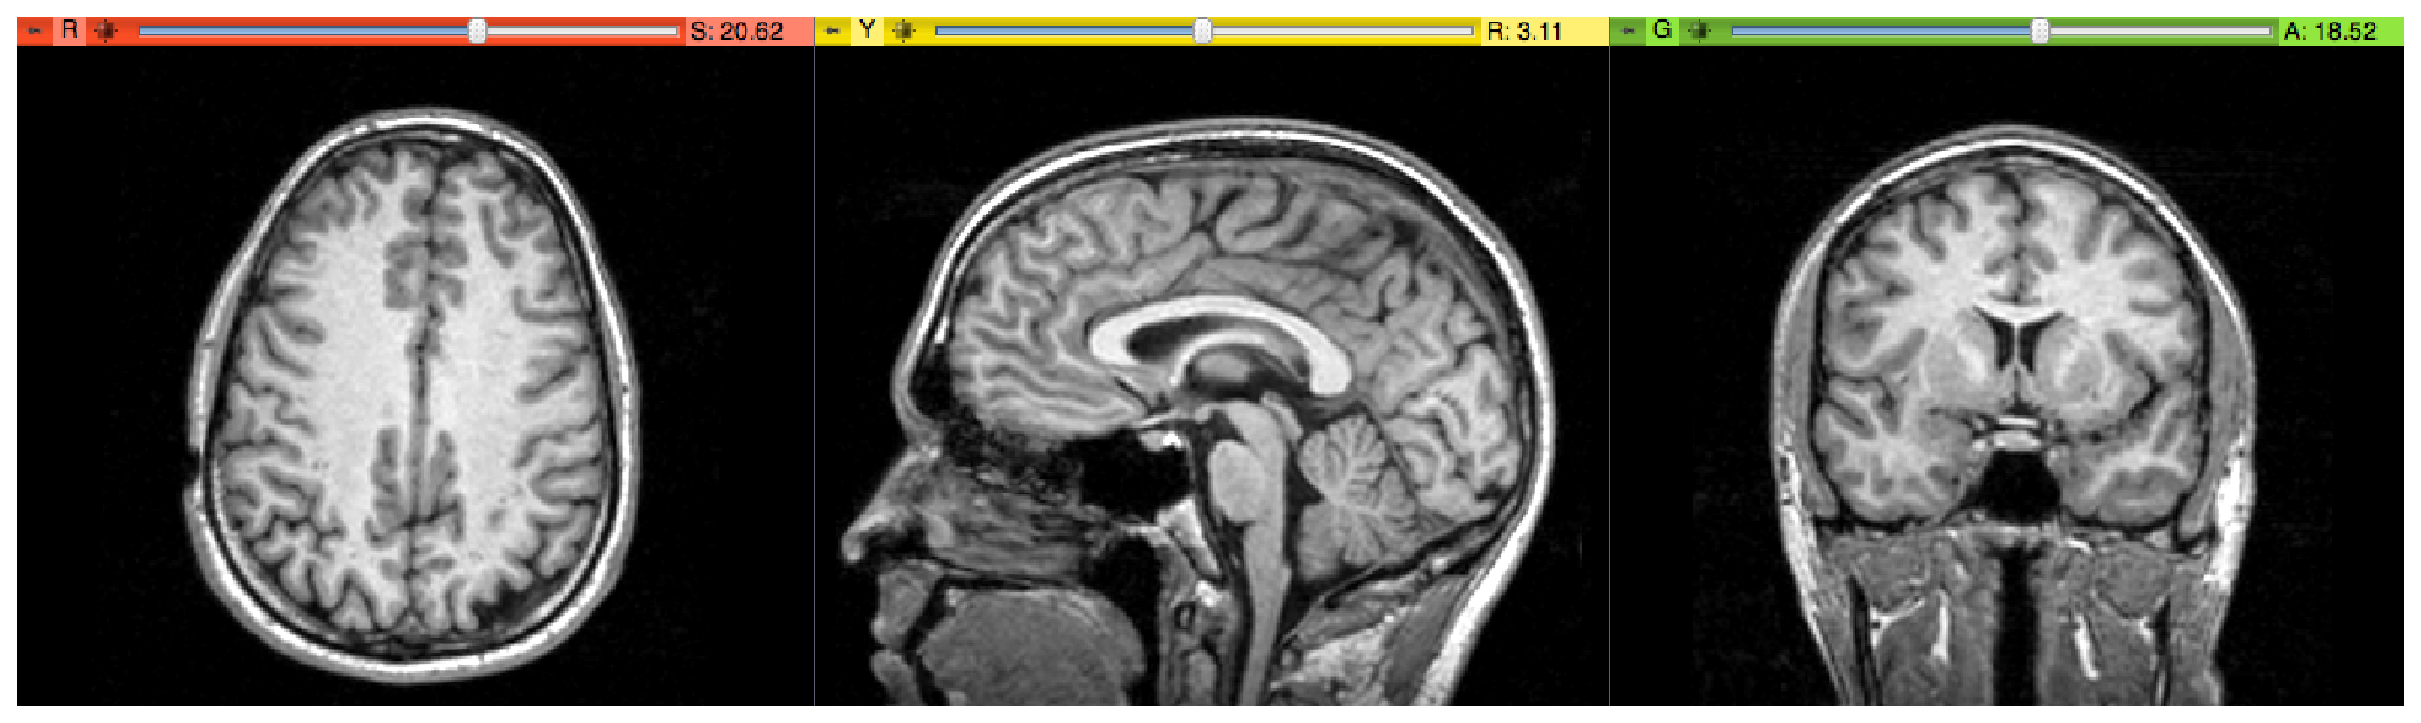
\includegraphics[scale=0.3]{/experiment_bigger/biggerA.eps}
  \caption{Large Differences: Baseline volume}
  \label{largeA}
\end{figure}

Cubes of large size where deleted from the follow-up volume to
represent areas of volume loss. The following volume was obtained:

\begin{figure}[H]
  \centering
  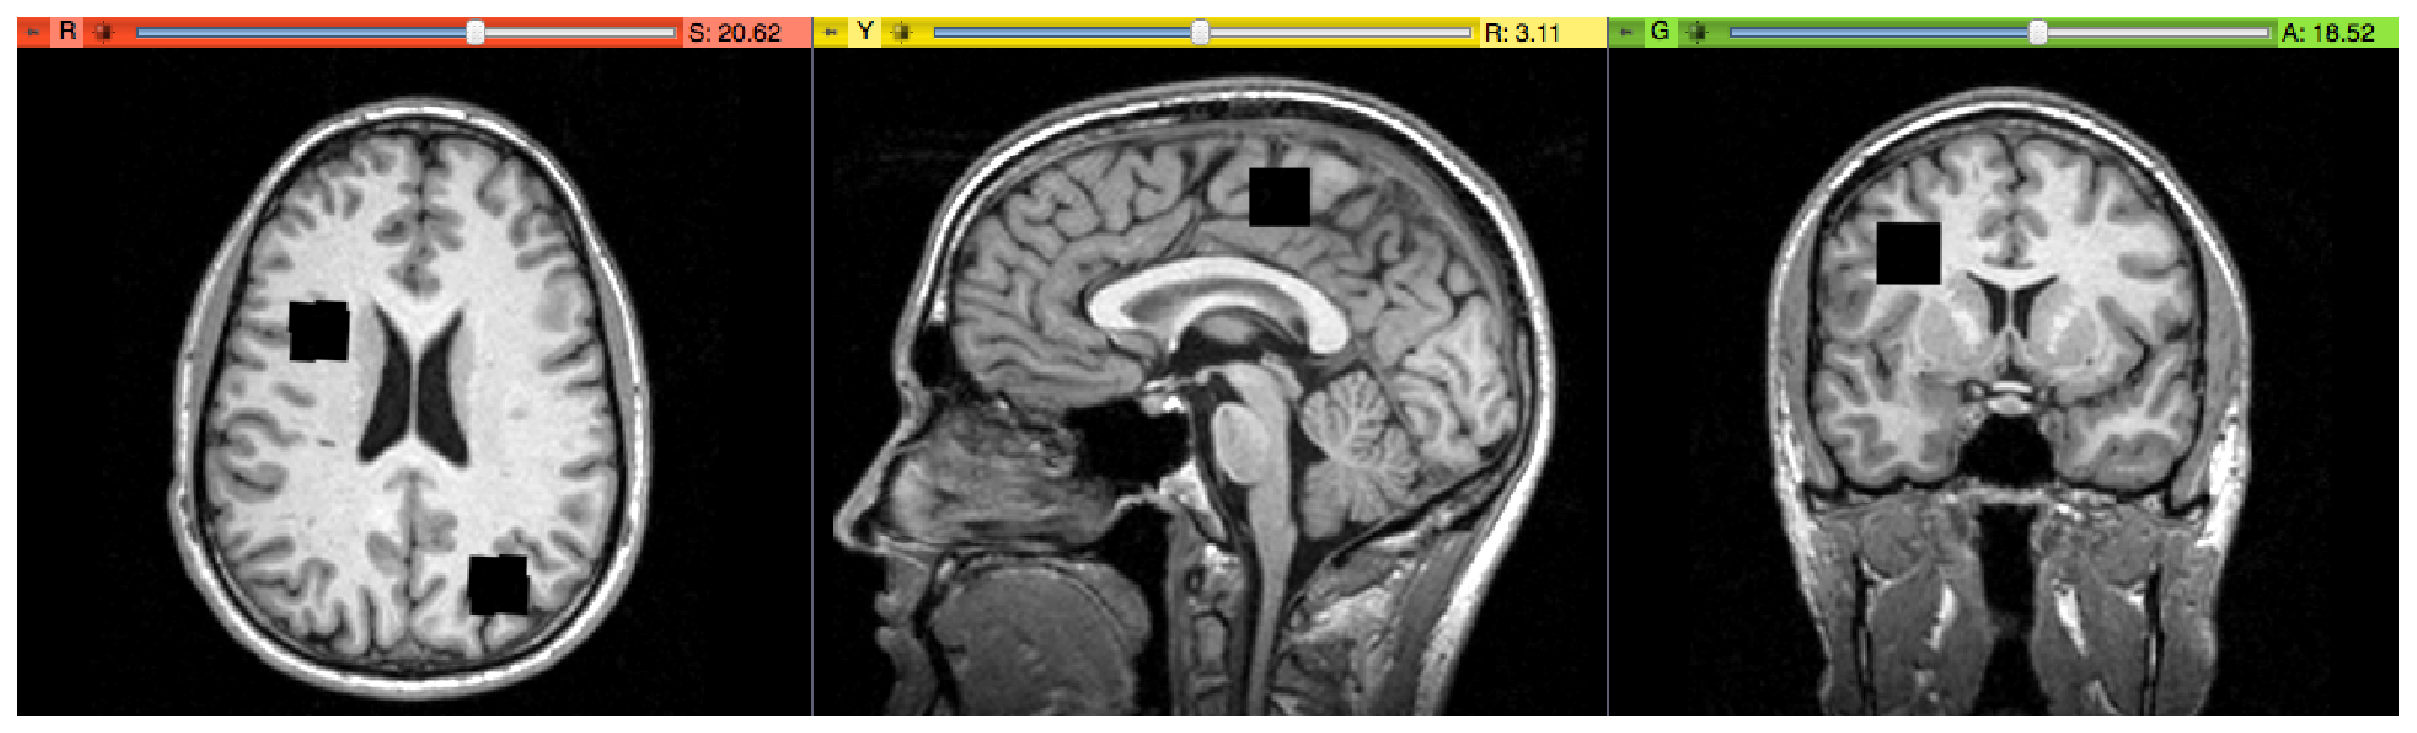
\includegraphics[scale=0.3]{/experiment_bigger/biggerB_subtracted.eps}
  \caption{Large Differences: Modified Follow-up volume}
  \label{largeB}
\end{figure}

\subsubsection{Voxel-based Method}
The result obtained with this method and large differences is pretty
good. All the differences are found and easy to see in the result.

\begin{figure}[H]
  \centering
  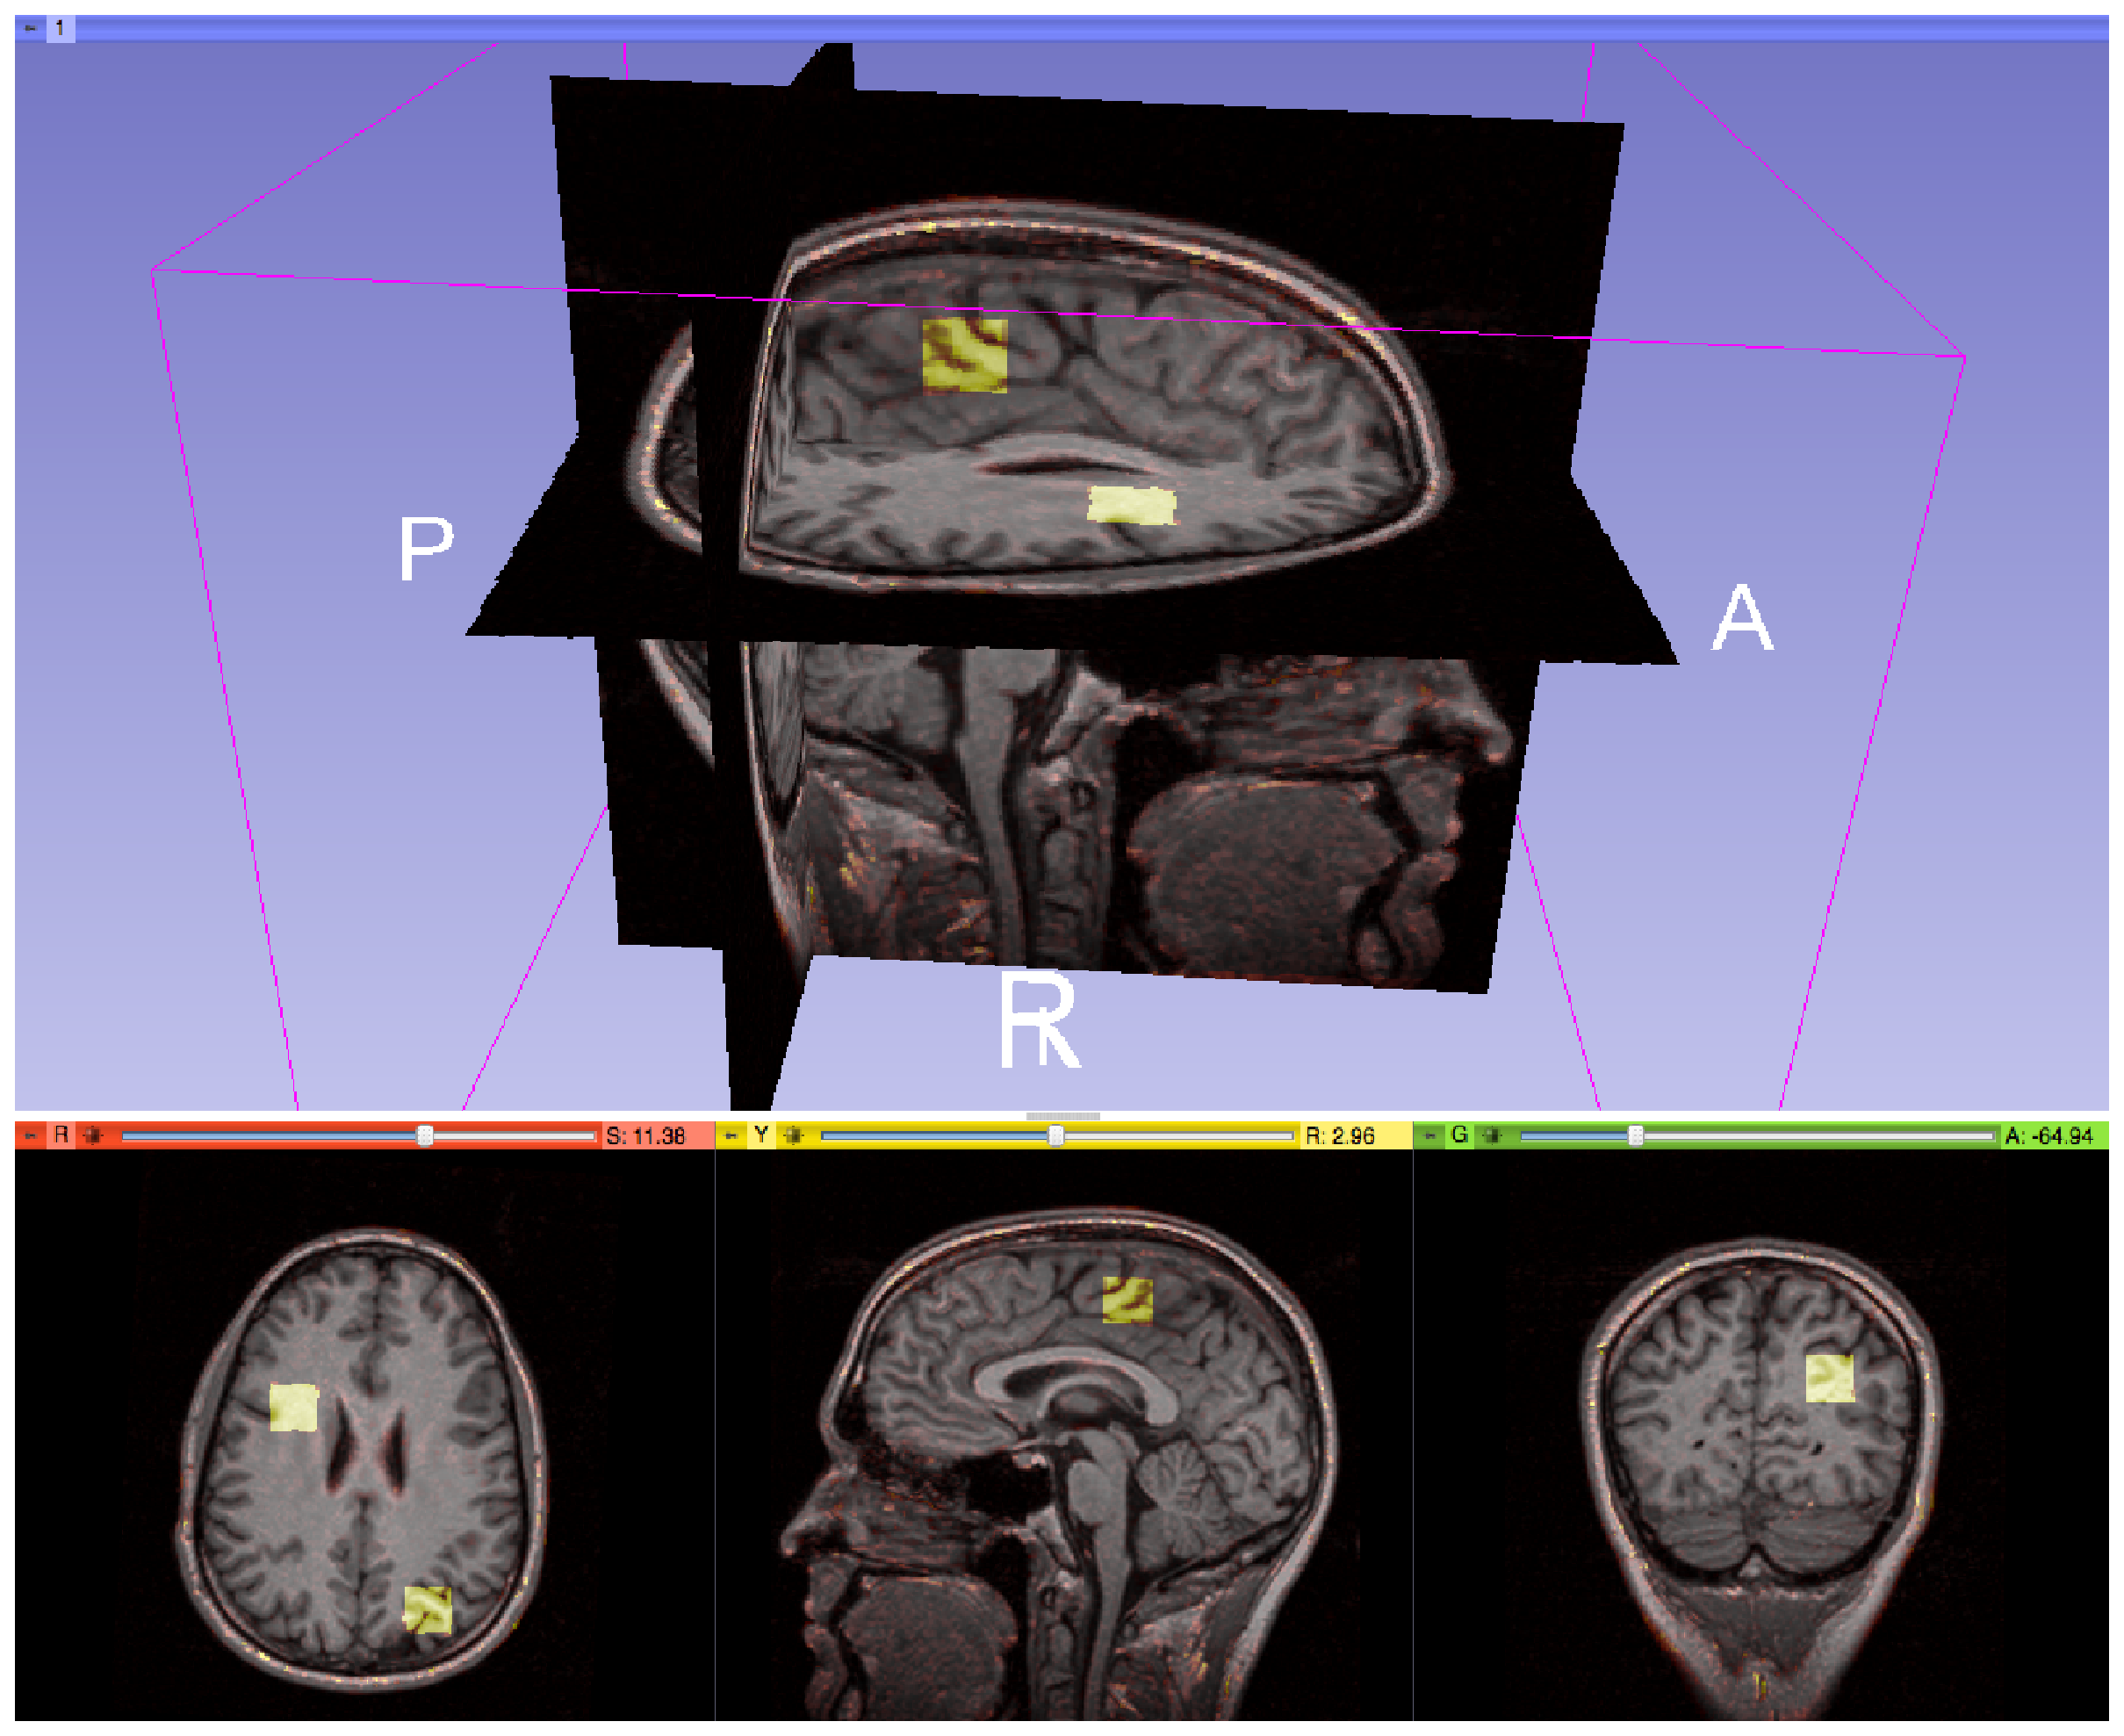
\includegraphics[scale=0.2]{/experiment_bigger/voxel_bigger1.eps}
  \caption{Artificial Large: Voxel-base method}
  \label{voxel_large1}
\end{figure}

Another angle of the result:

\begin{figure}[H]
  \centering
  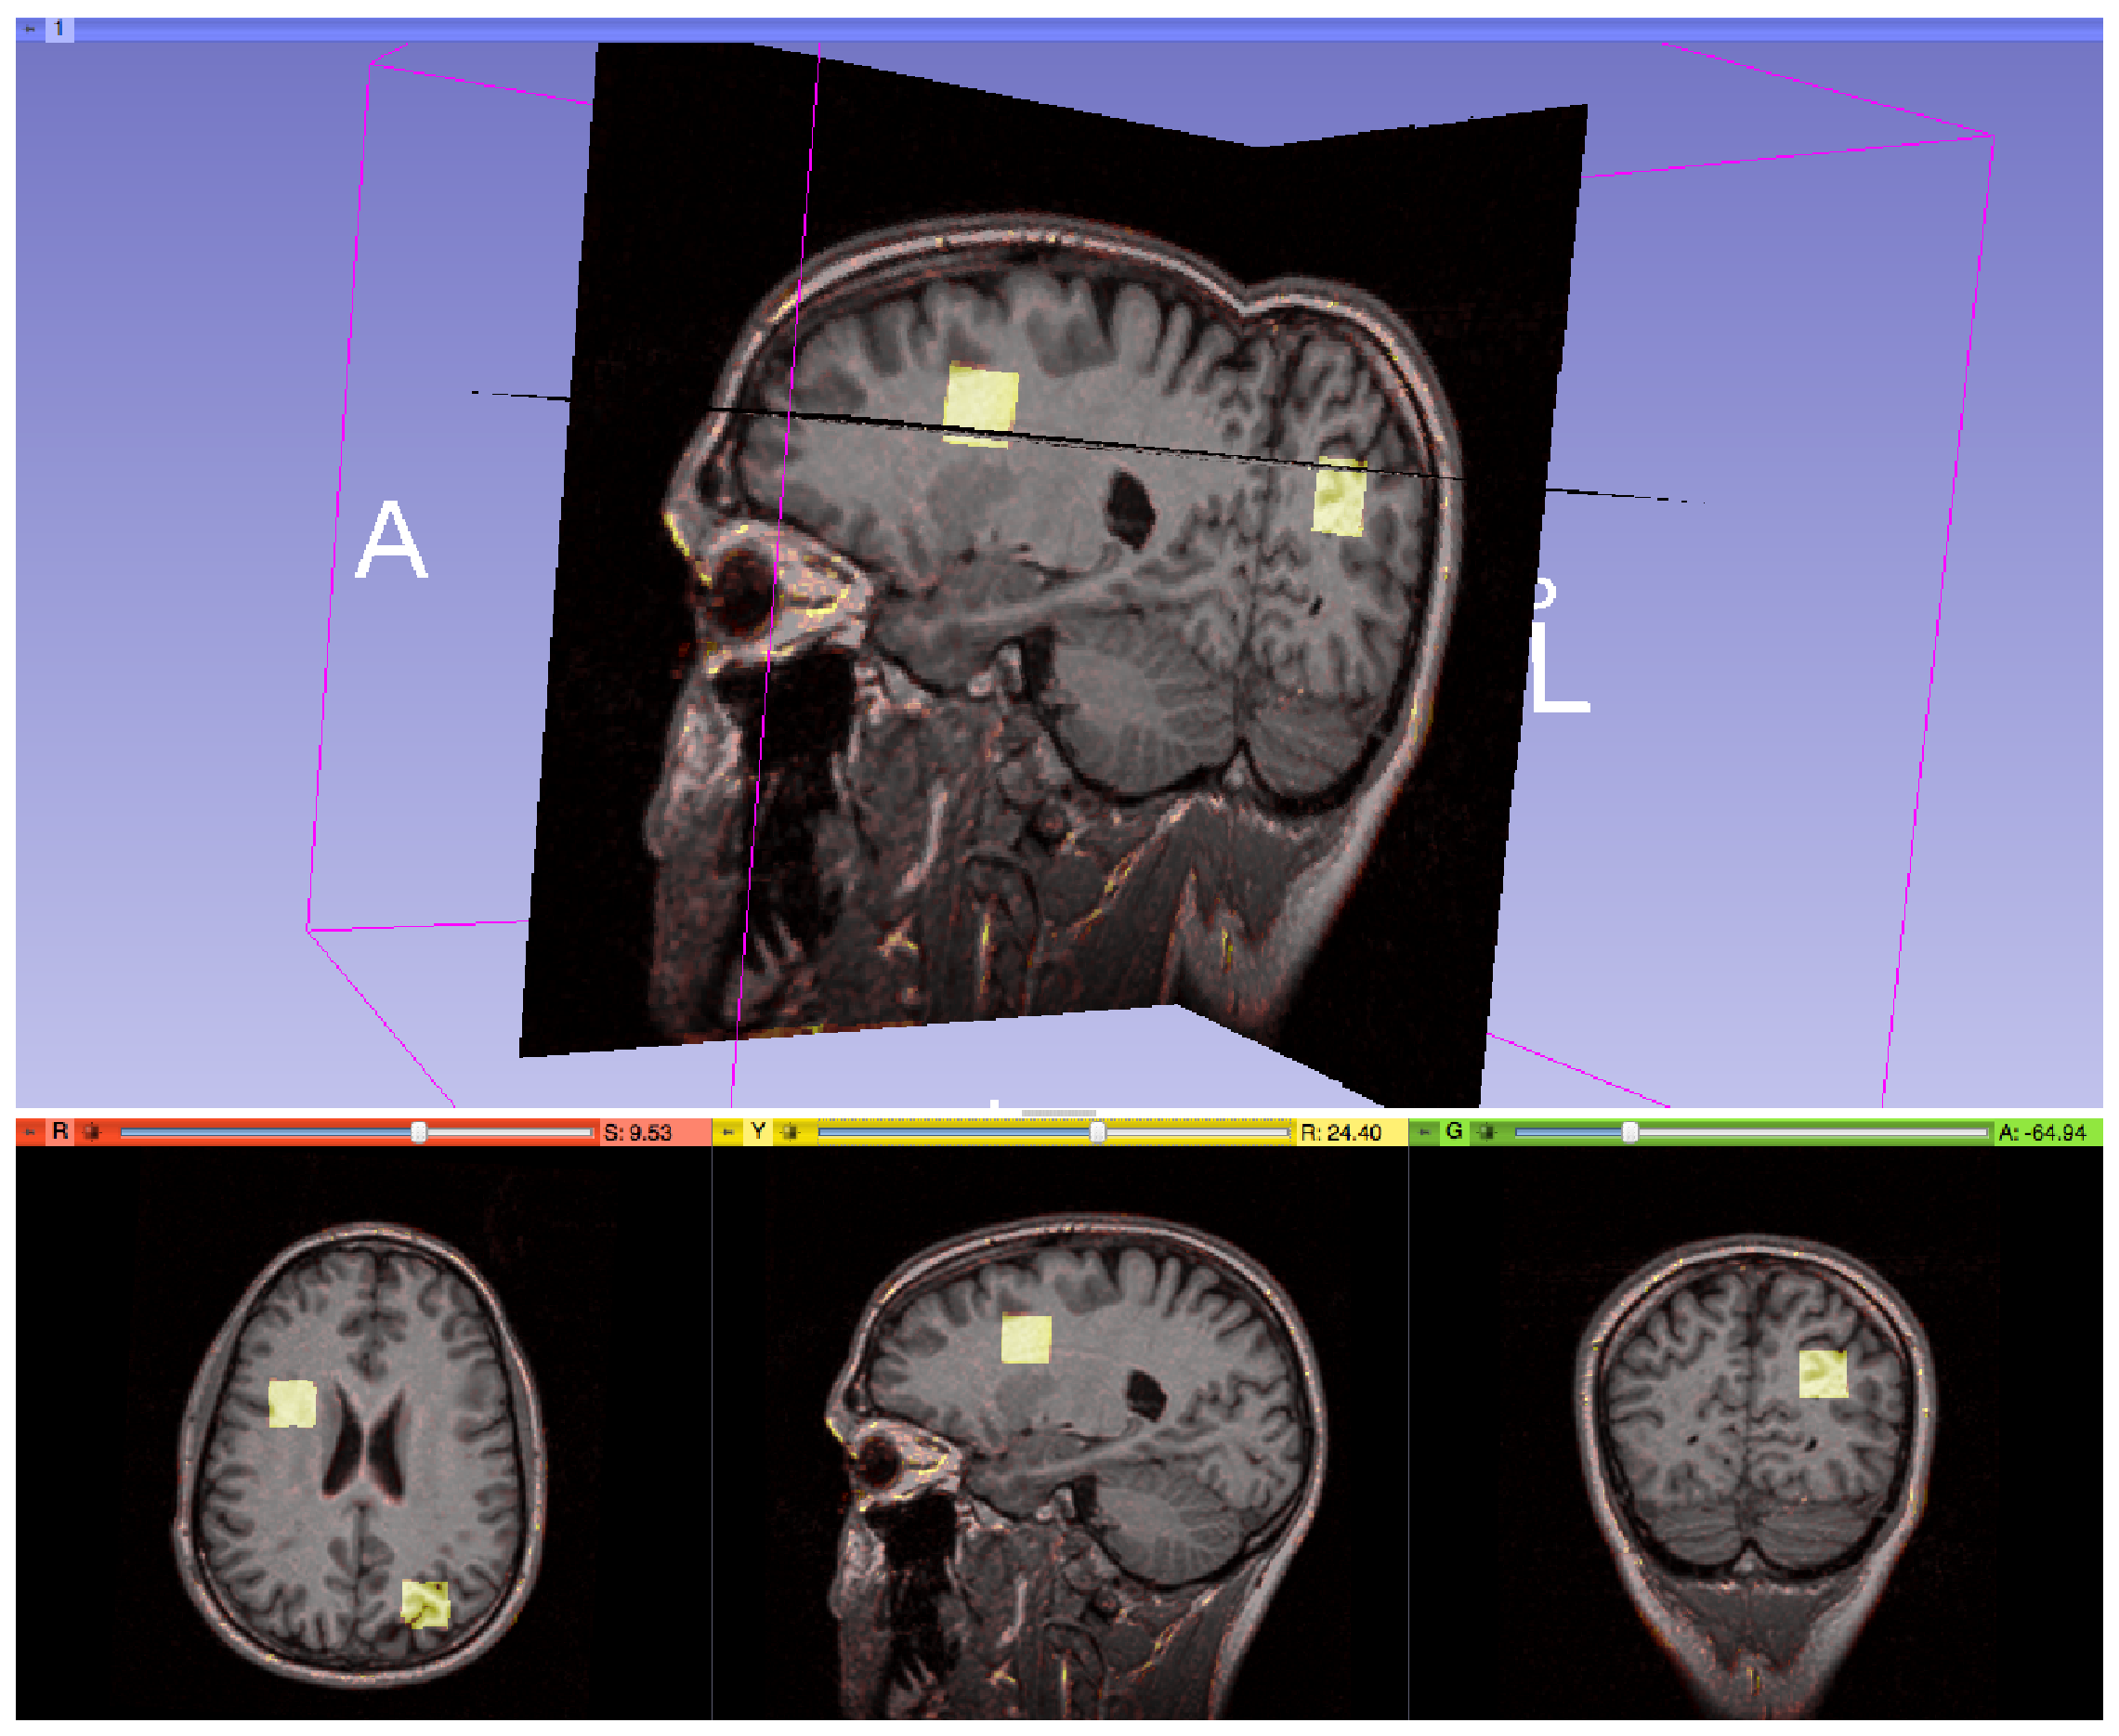
\includegraphics[scale=0.2]{/experiment_bigger/voxel_bigger2.eps}
  \caption{Artificial Large: Voxel-base method}
  \label{voxel_large2}
\end{figure}

\subsubsection{Tensor-based Method}
In the result obtained with this method the differences are easy to
find, but their borders are not properly defined. The method gives the
position of the differences but not their exact shape.

The parameters used to obtain this result are:
\begin{description}
\item \textit{Deformation field smoothing sigma:} 2.5
\item \textit{Shrinkage percentage:} 80
\item \textit{Growth percentage:} 65
\end{description}

\begin{figure}[H]
  \centering
  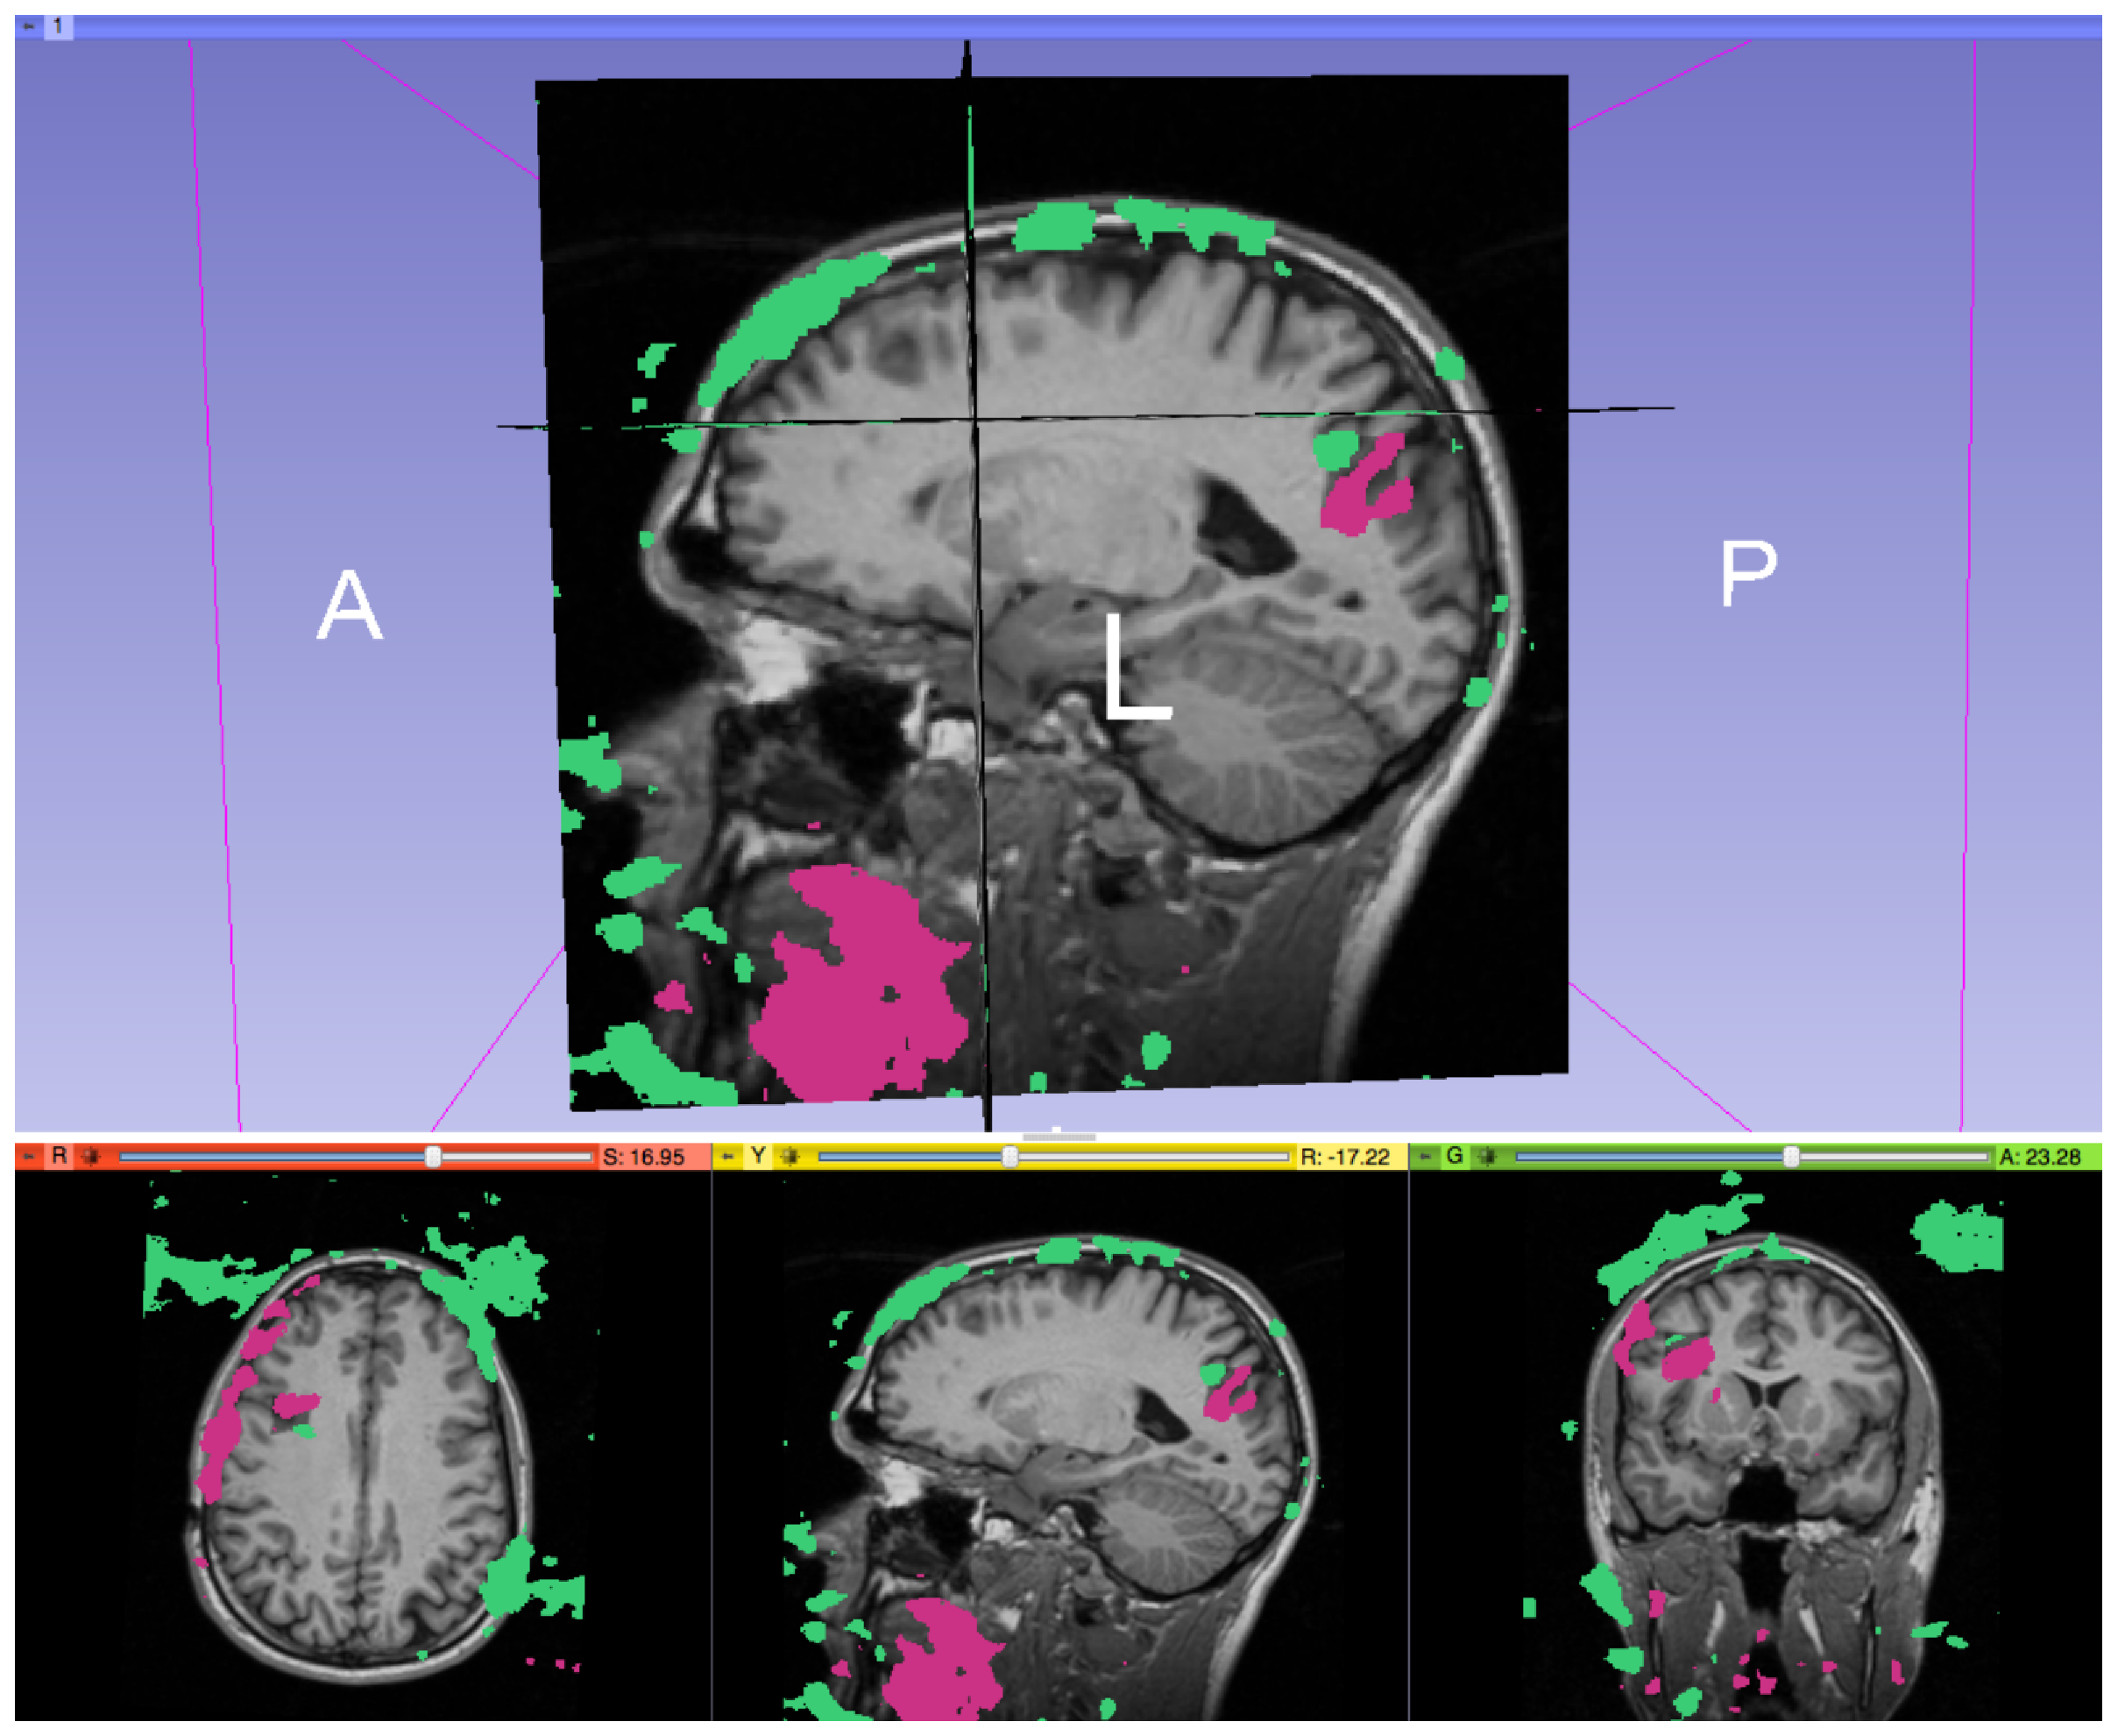
\includegraphics[scale=0.2]{/experiment_bigger/tensor80-65_bigger1.eps}
  \caption{Artificial Large: Tensor-base method}
  \label{voxel_large1}
\end{figure}

Another angle of the result:

\begin{figure}[H]
  \centering
  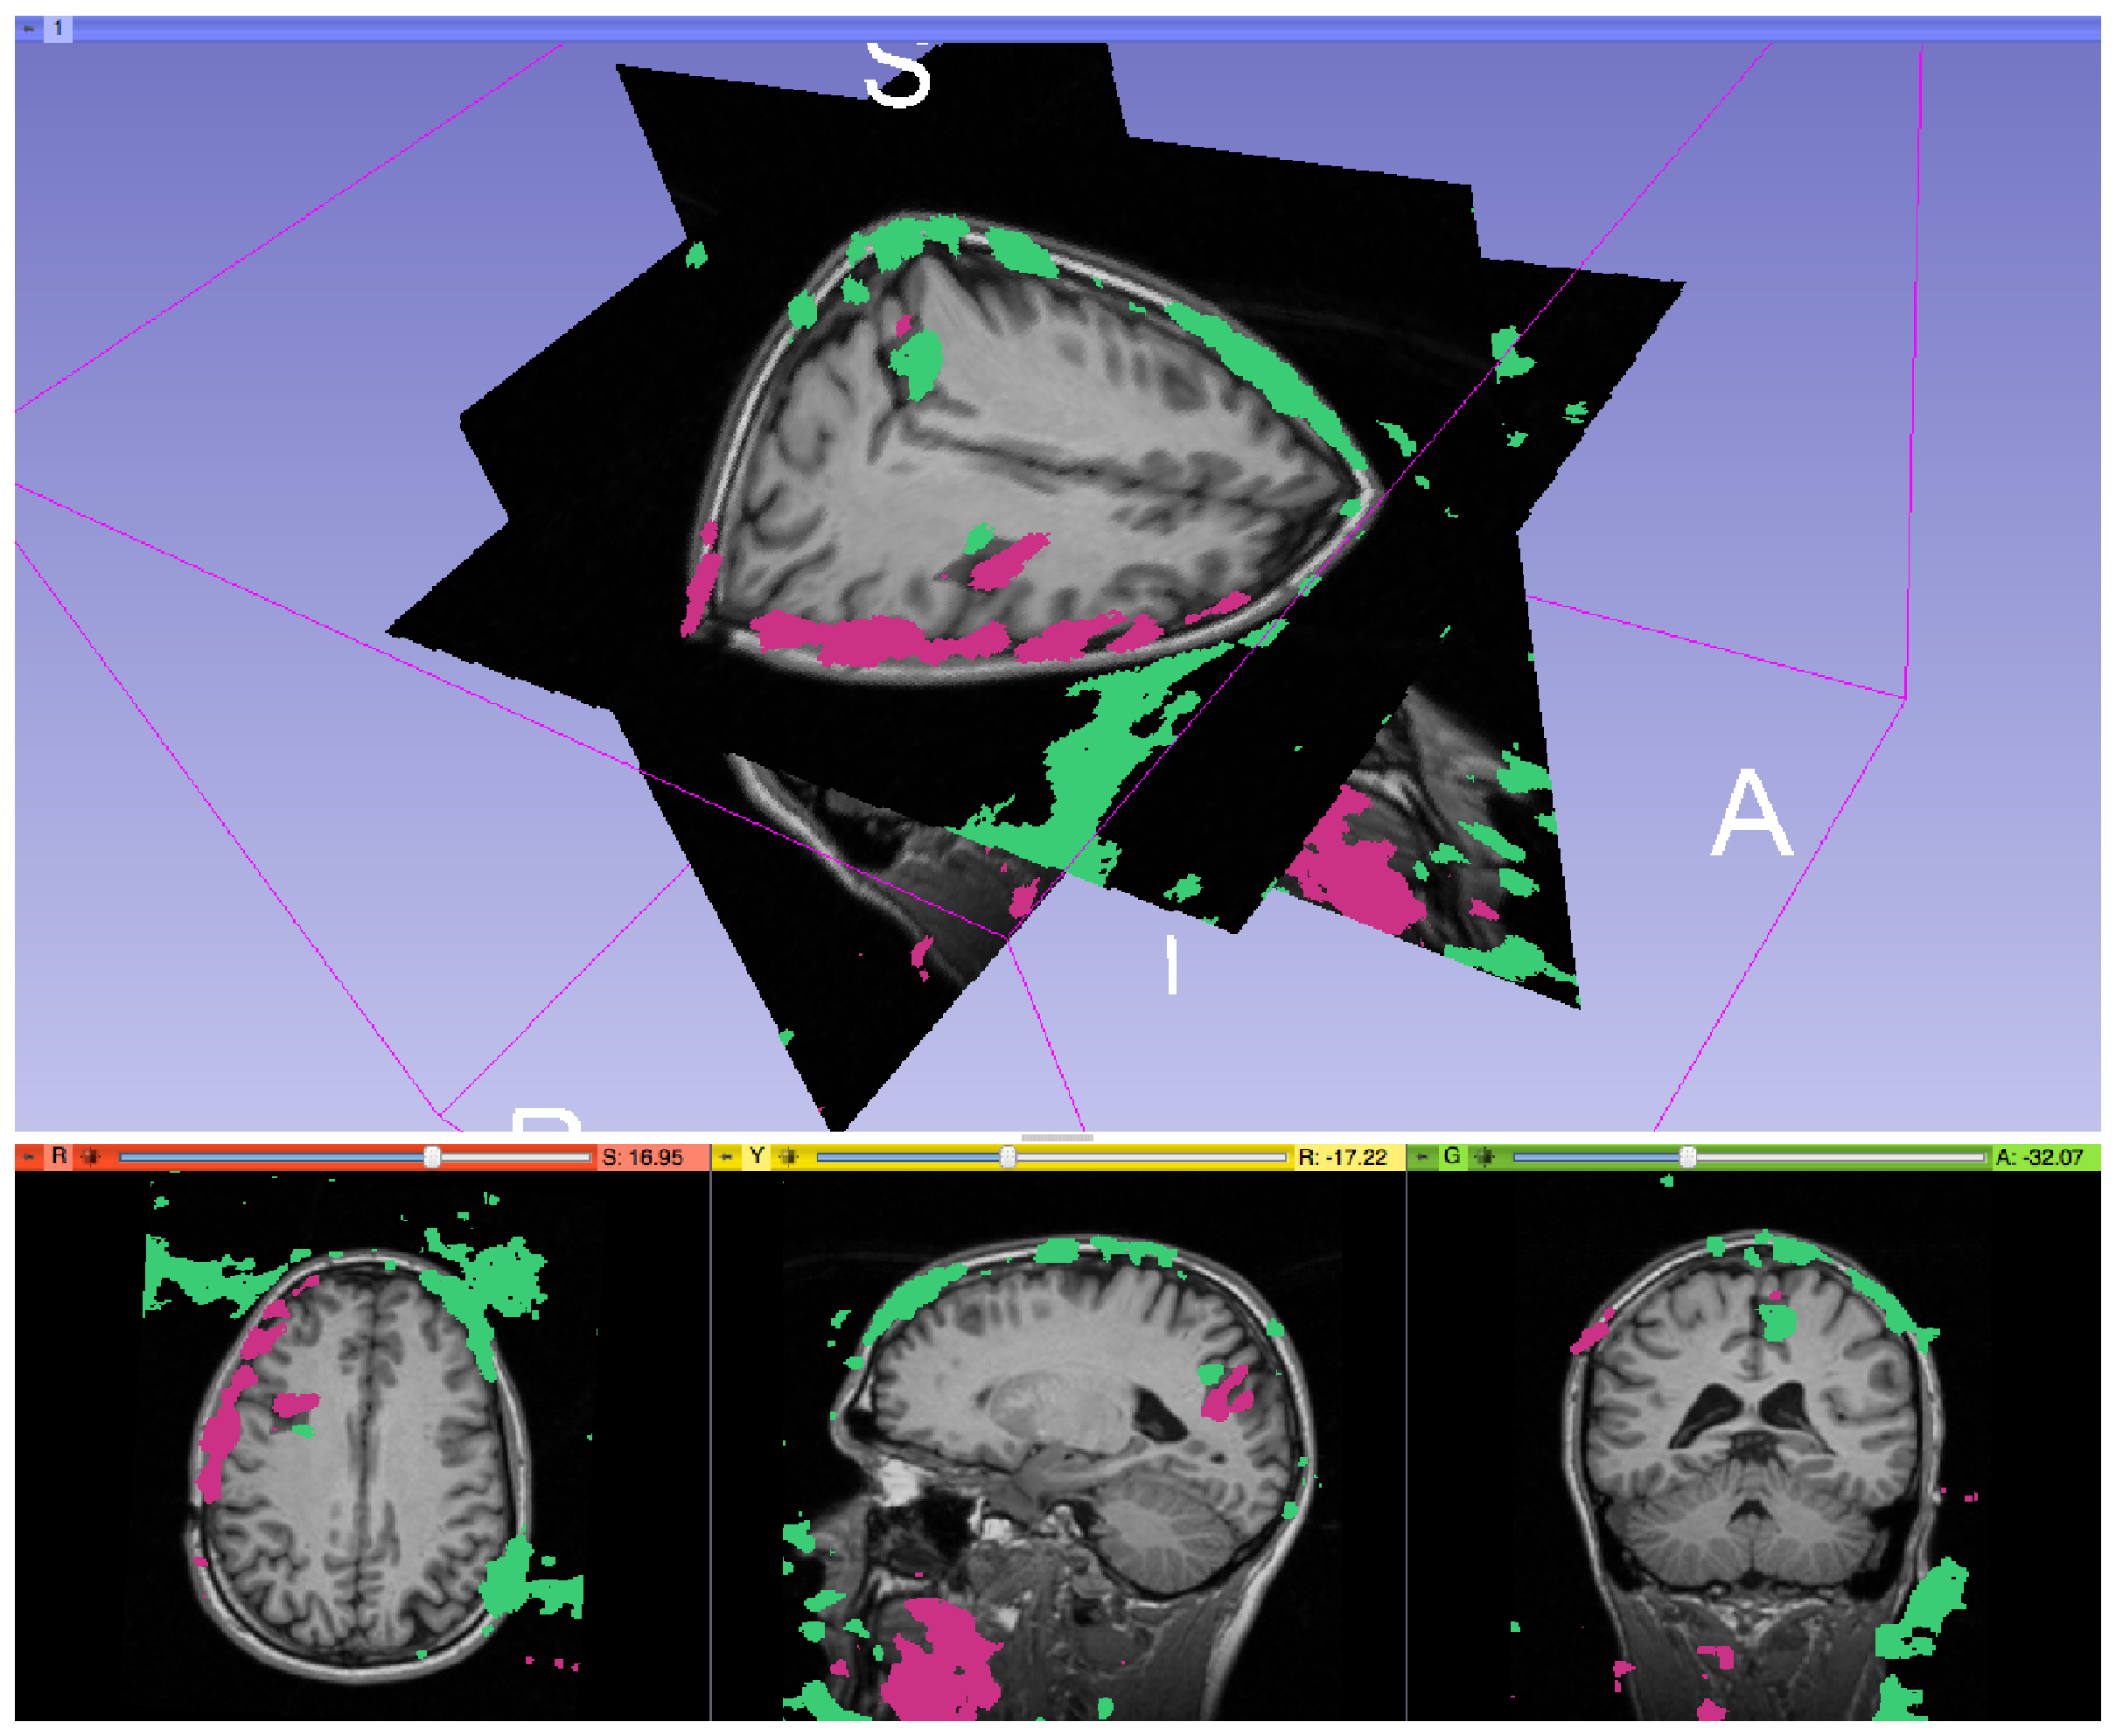
\includegraphics[scale=0.2]{/experiment_bigger/tensor80_65_bigger2.eps}
  \caption{Artificial Large: Tensor-base method}
  \label{voxel_large2}
\end{figure}


\subsection{Size: Medium}
\subsubsection{Voxel-based Method}

\subsubsection{Tensor-based Method}


\subsection{Size: Small}
\subsubsection{Voxel-based Method}




\subsubsection{Tensor-based Method}


\section{Real Differences Results}

\subsection{Patient 1}
This patient presents small differences in the parietal lobe, the
differences can be seen as red lines in the voxel-based method's result
and pink or green areas in the tensor-based method's result.

\subsubsection{Voxel-based Method}
The registration method used was \textit{Affine registration}.

\begin{figure}[H]
  \centering
  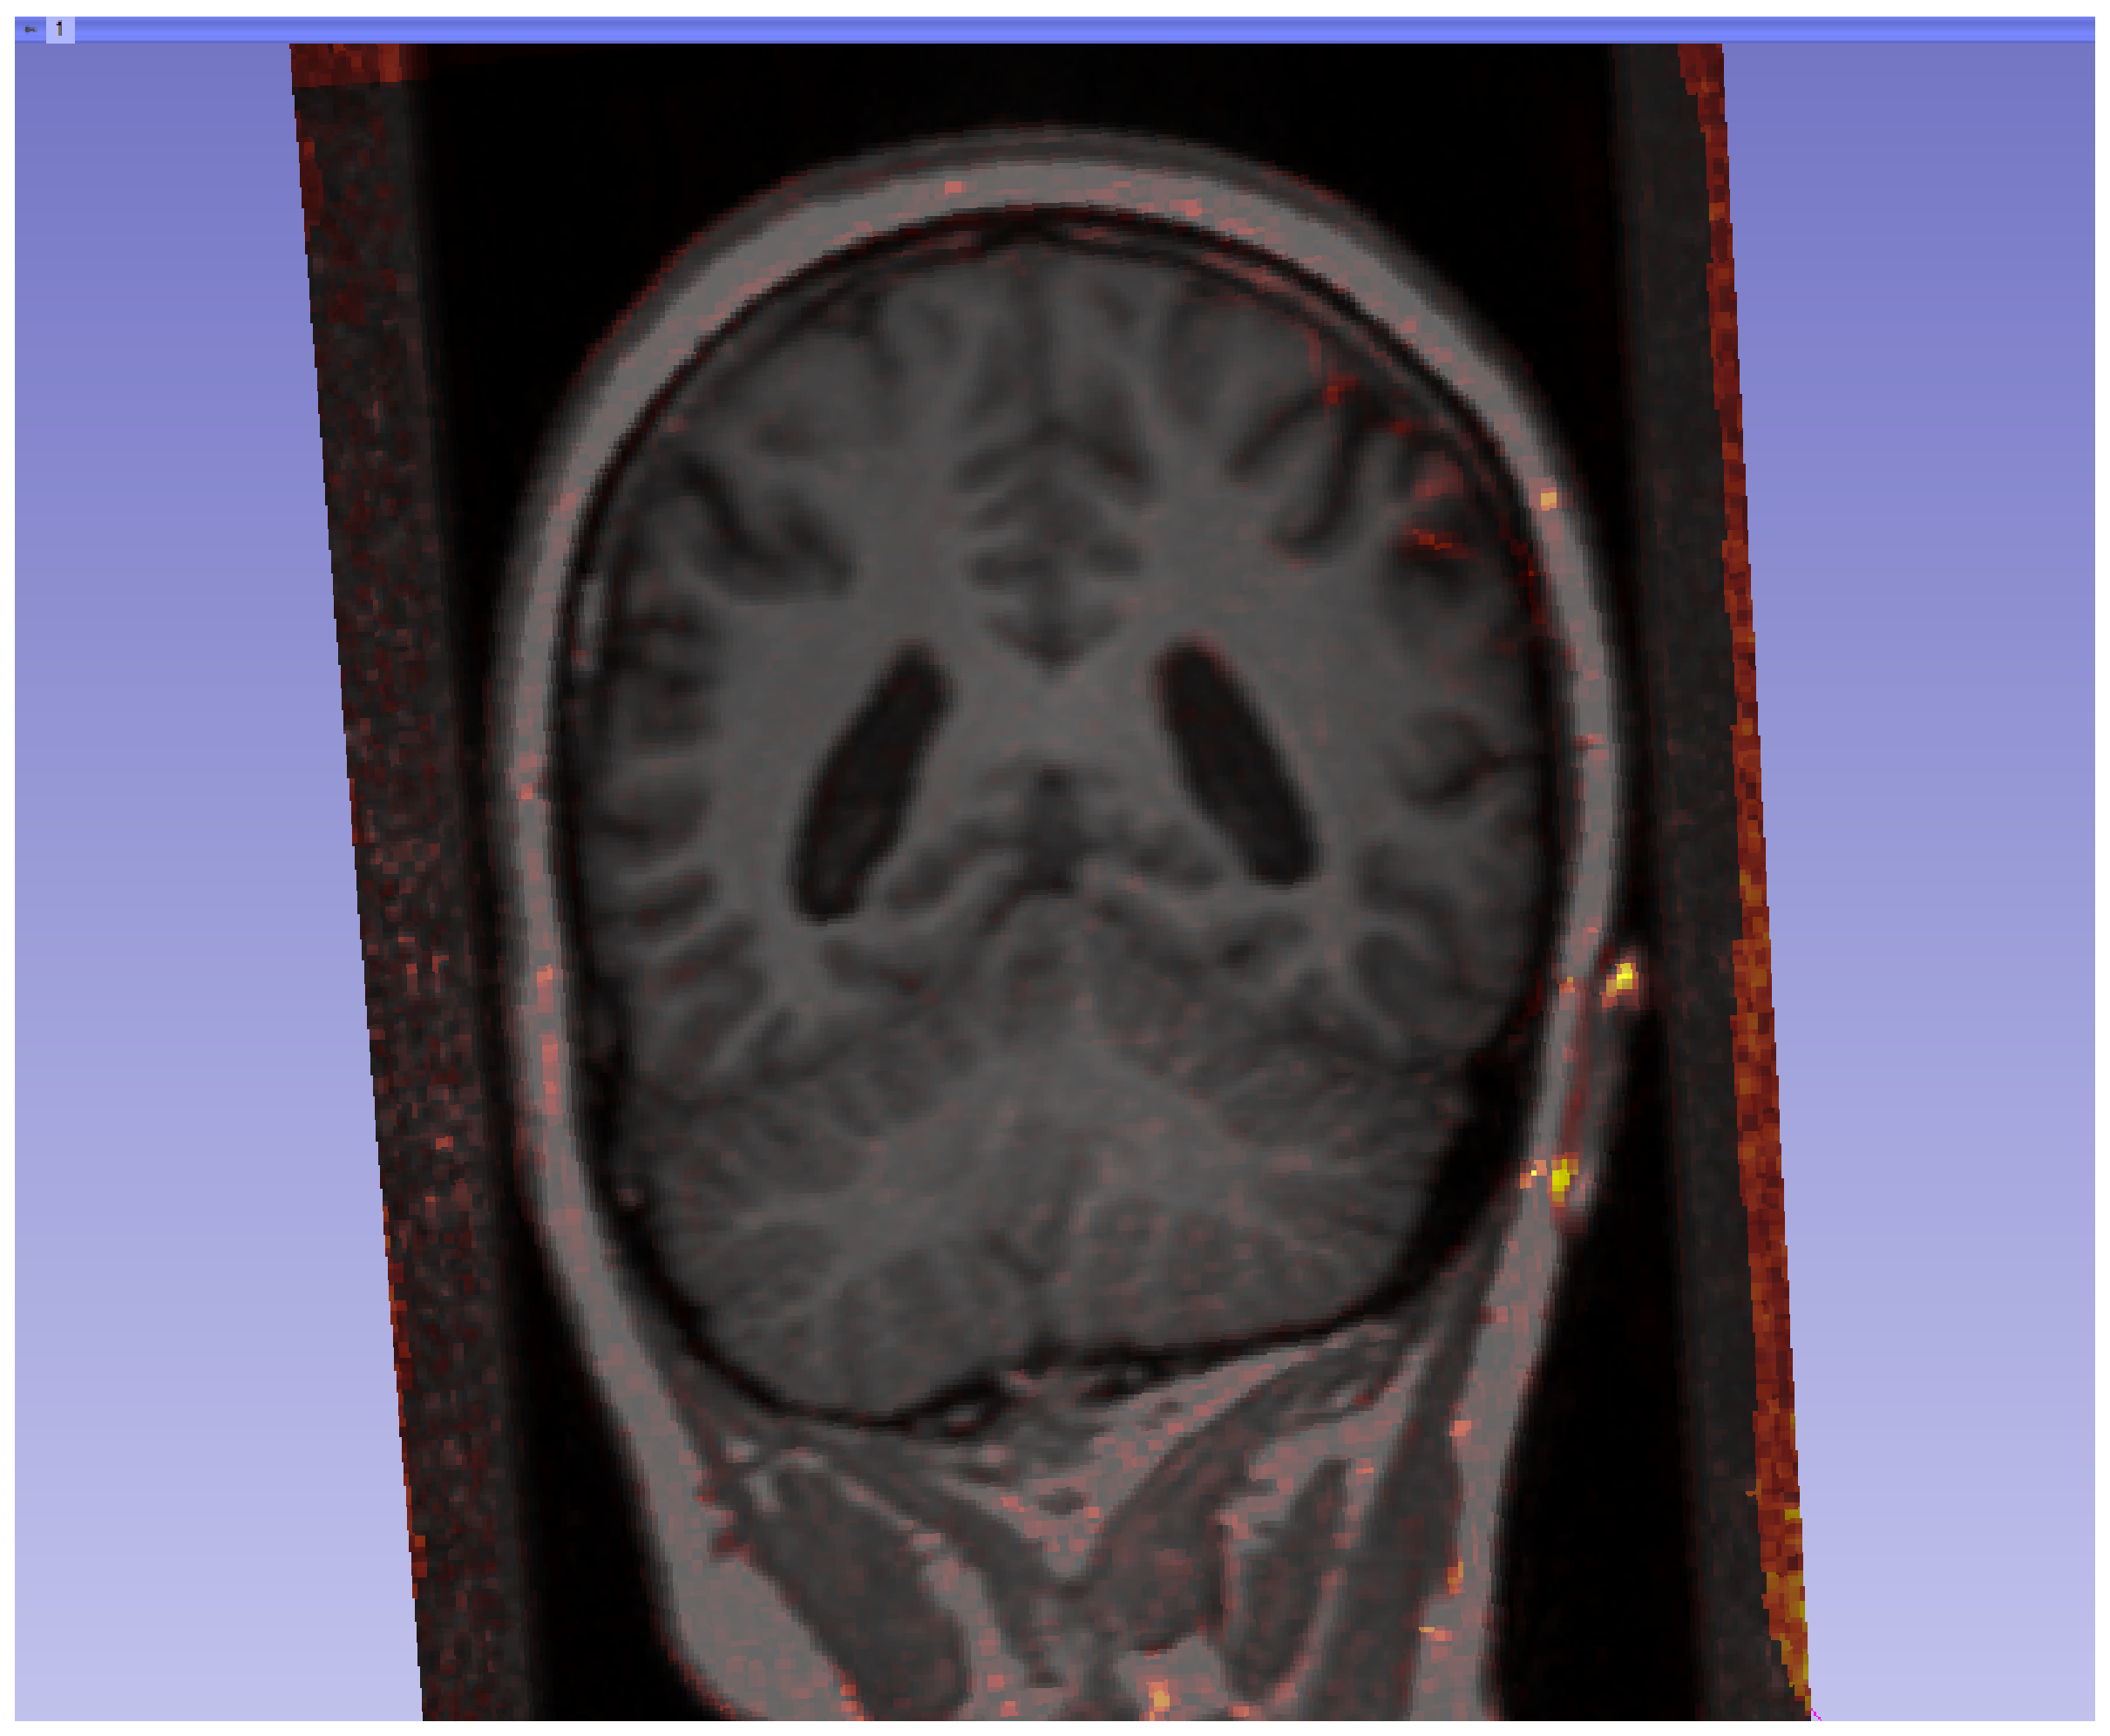
\includegraphics[scale=0.2]{/experiment_CL_P1/CL_Coronal.eps}
  \caption{Voxel-based method. Patient 1: Coronal plane}
  \label{CL_Coronal}
\end{figure}

\begin{figure}[H]
  \centering
  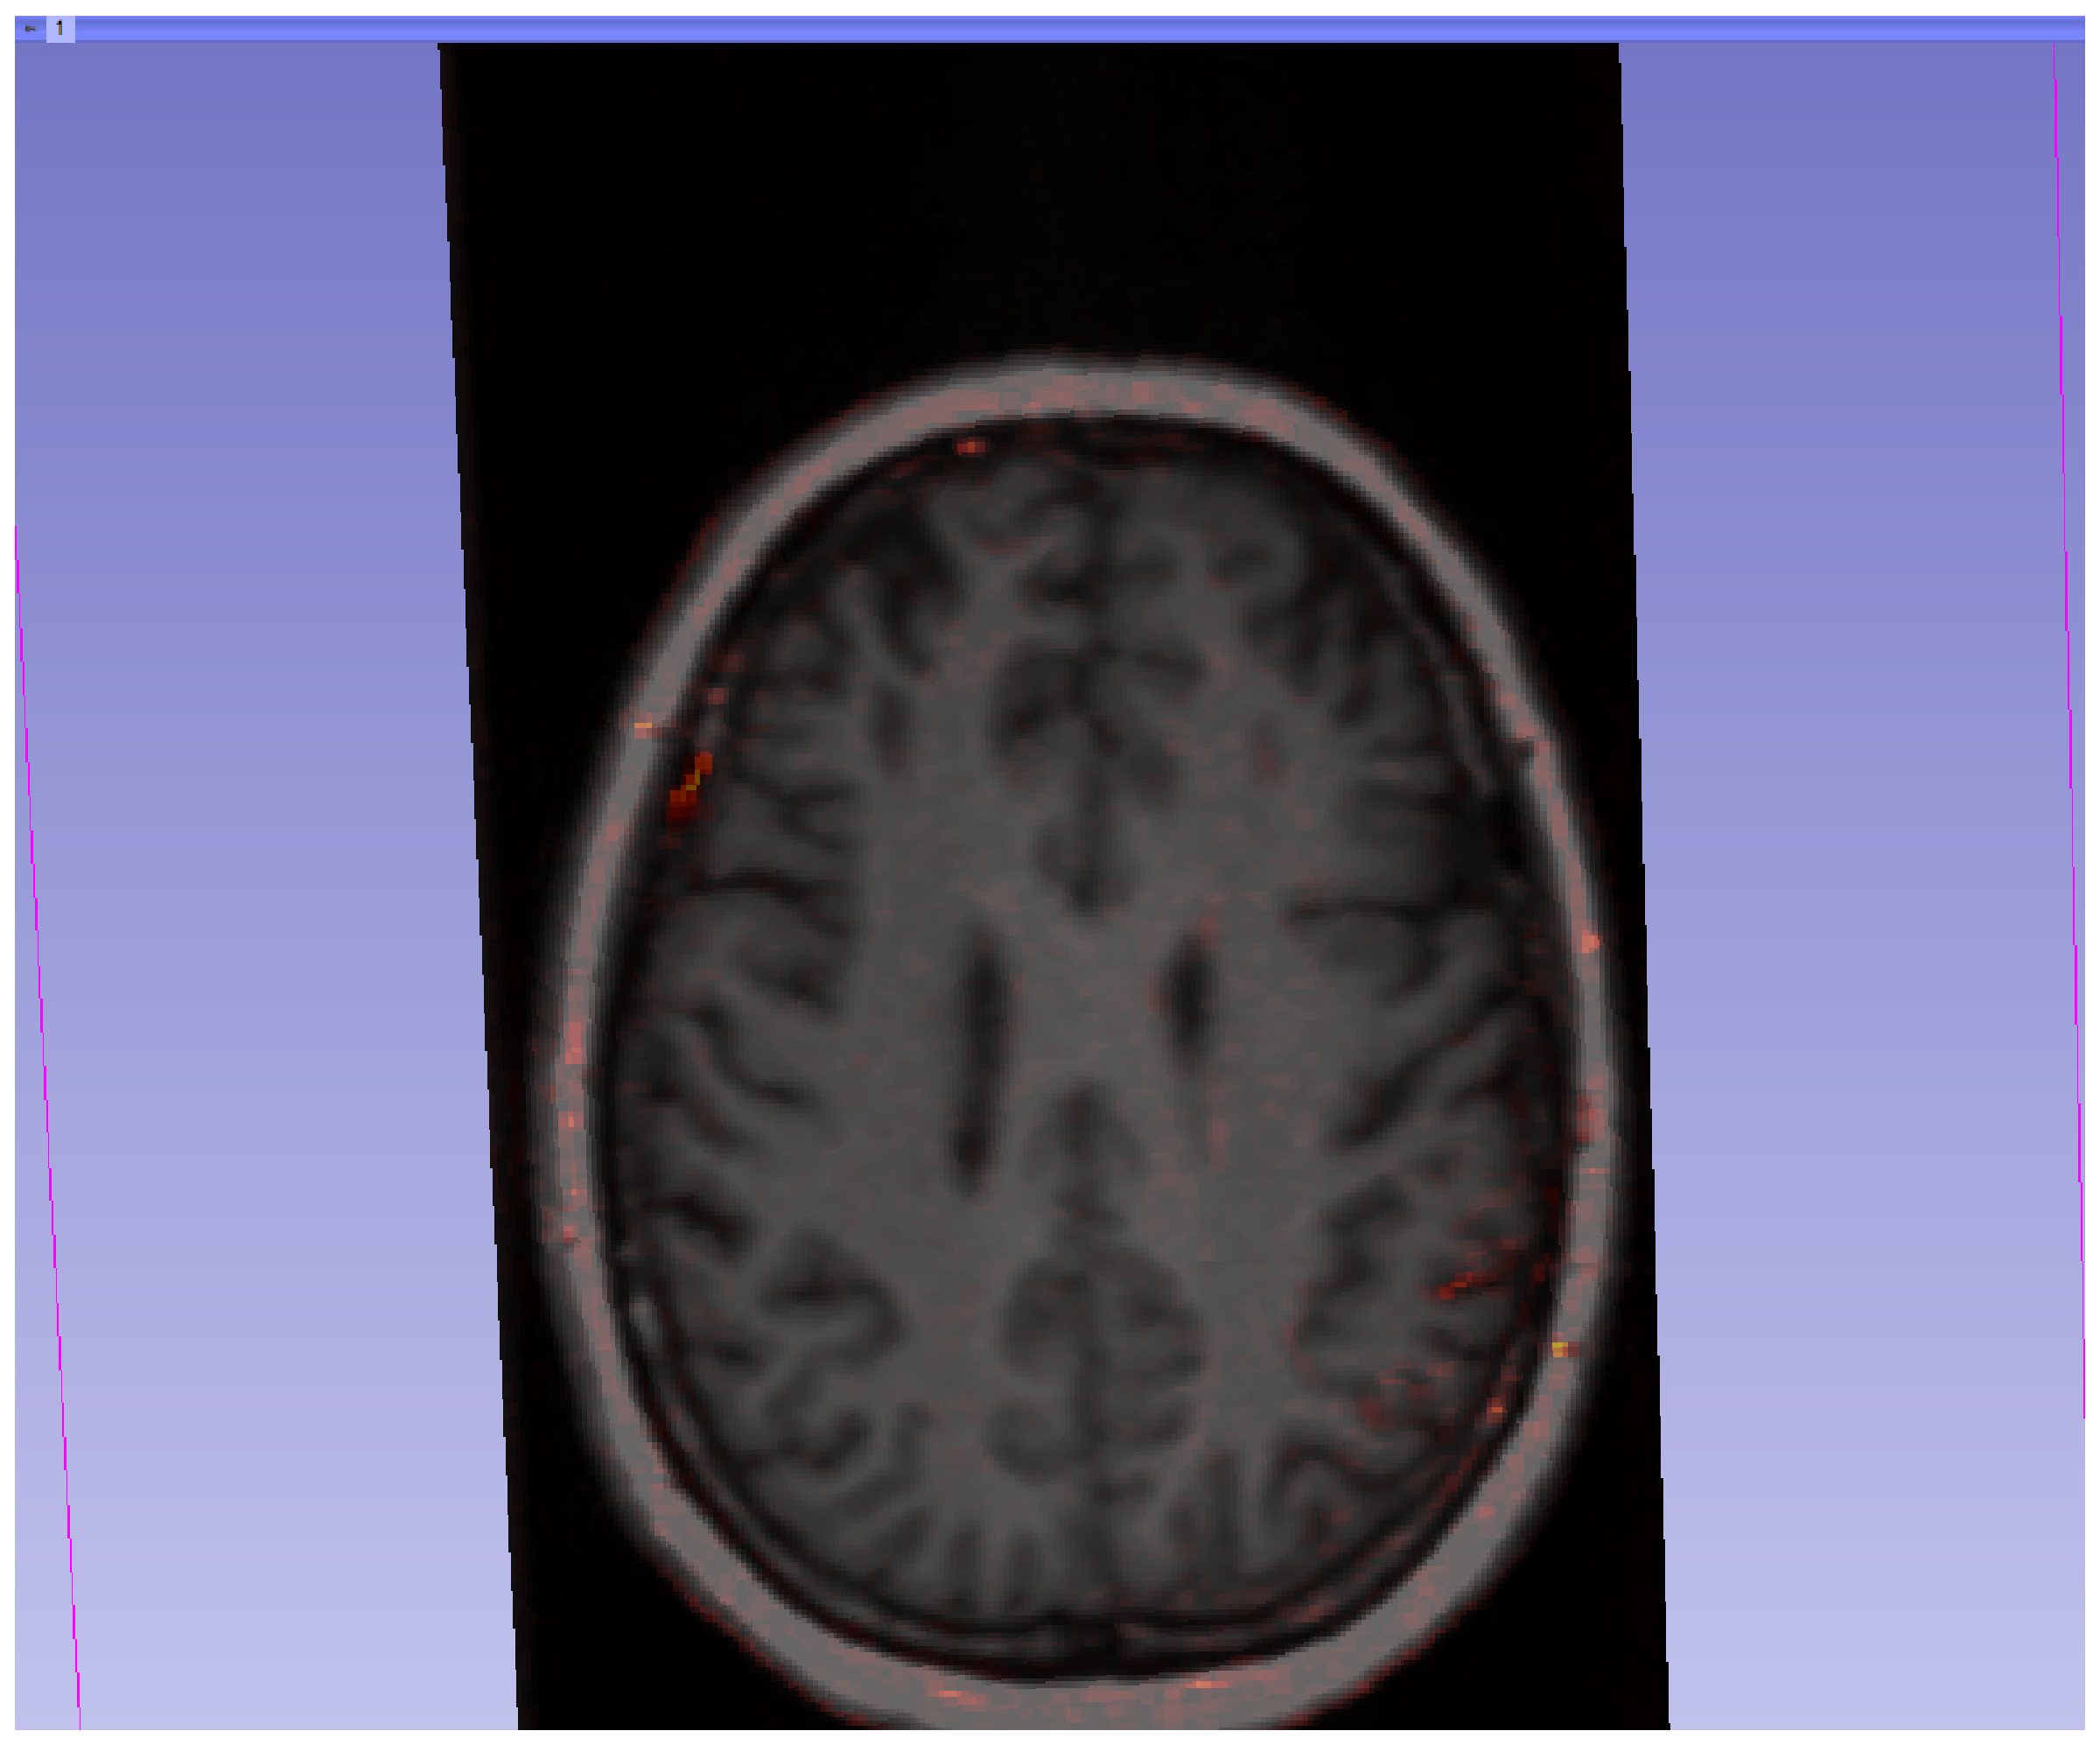
\includegraphics[scale=0.2]{/experiment_CL_P1/CL_Traversal.eps}
  \caption{Voxel-based method. Patient 1: Traversal plane}
  \label{CL_Traversal}
\end{figure}

\begin{figure}[H]
  \centering
  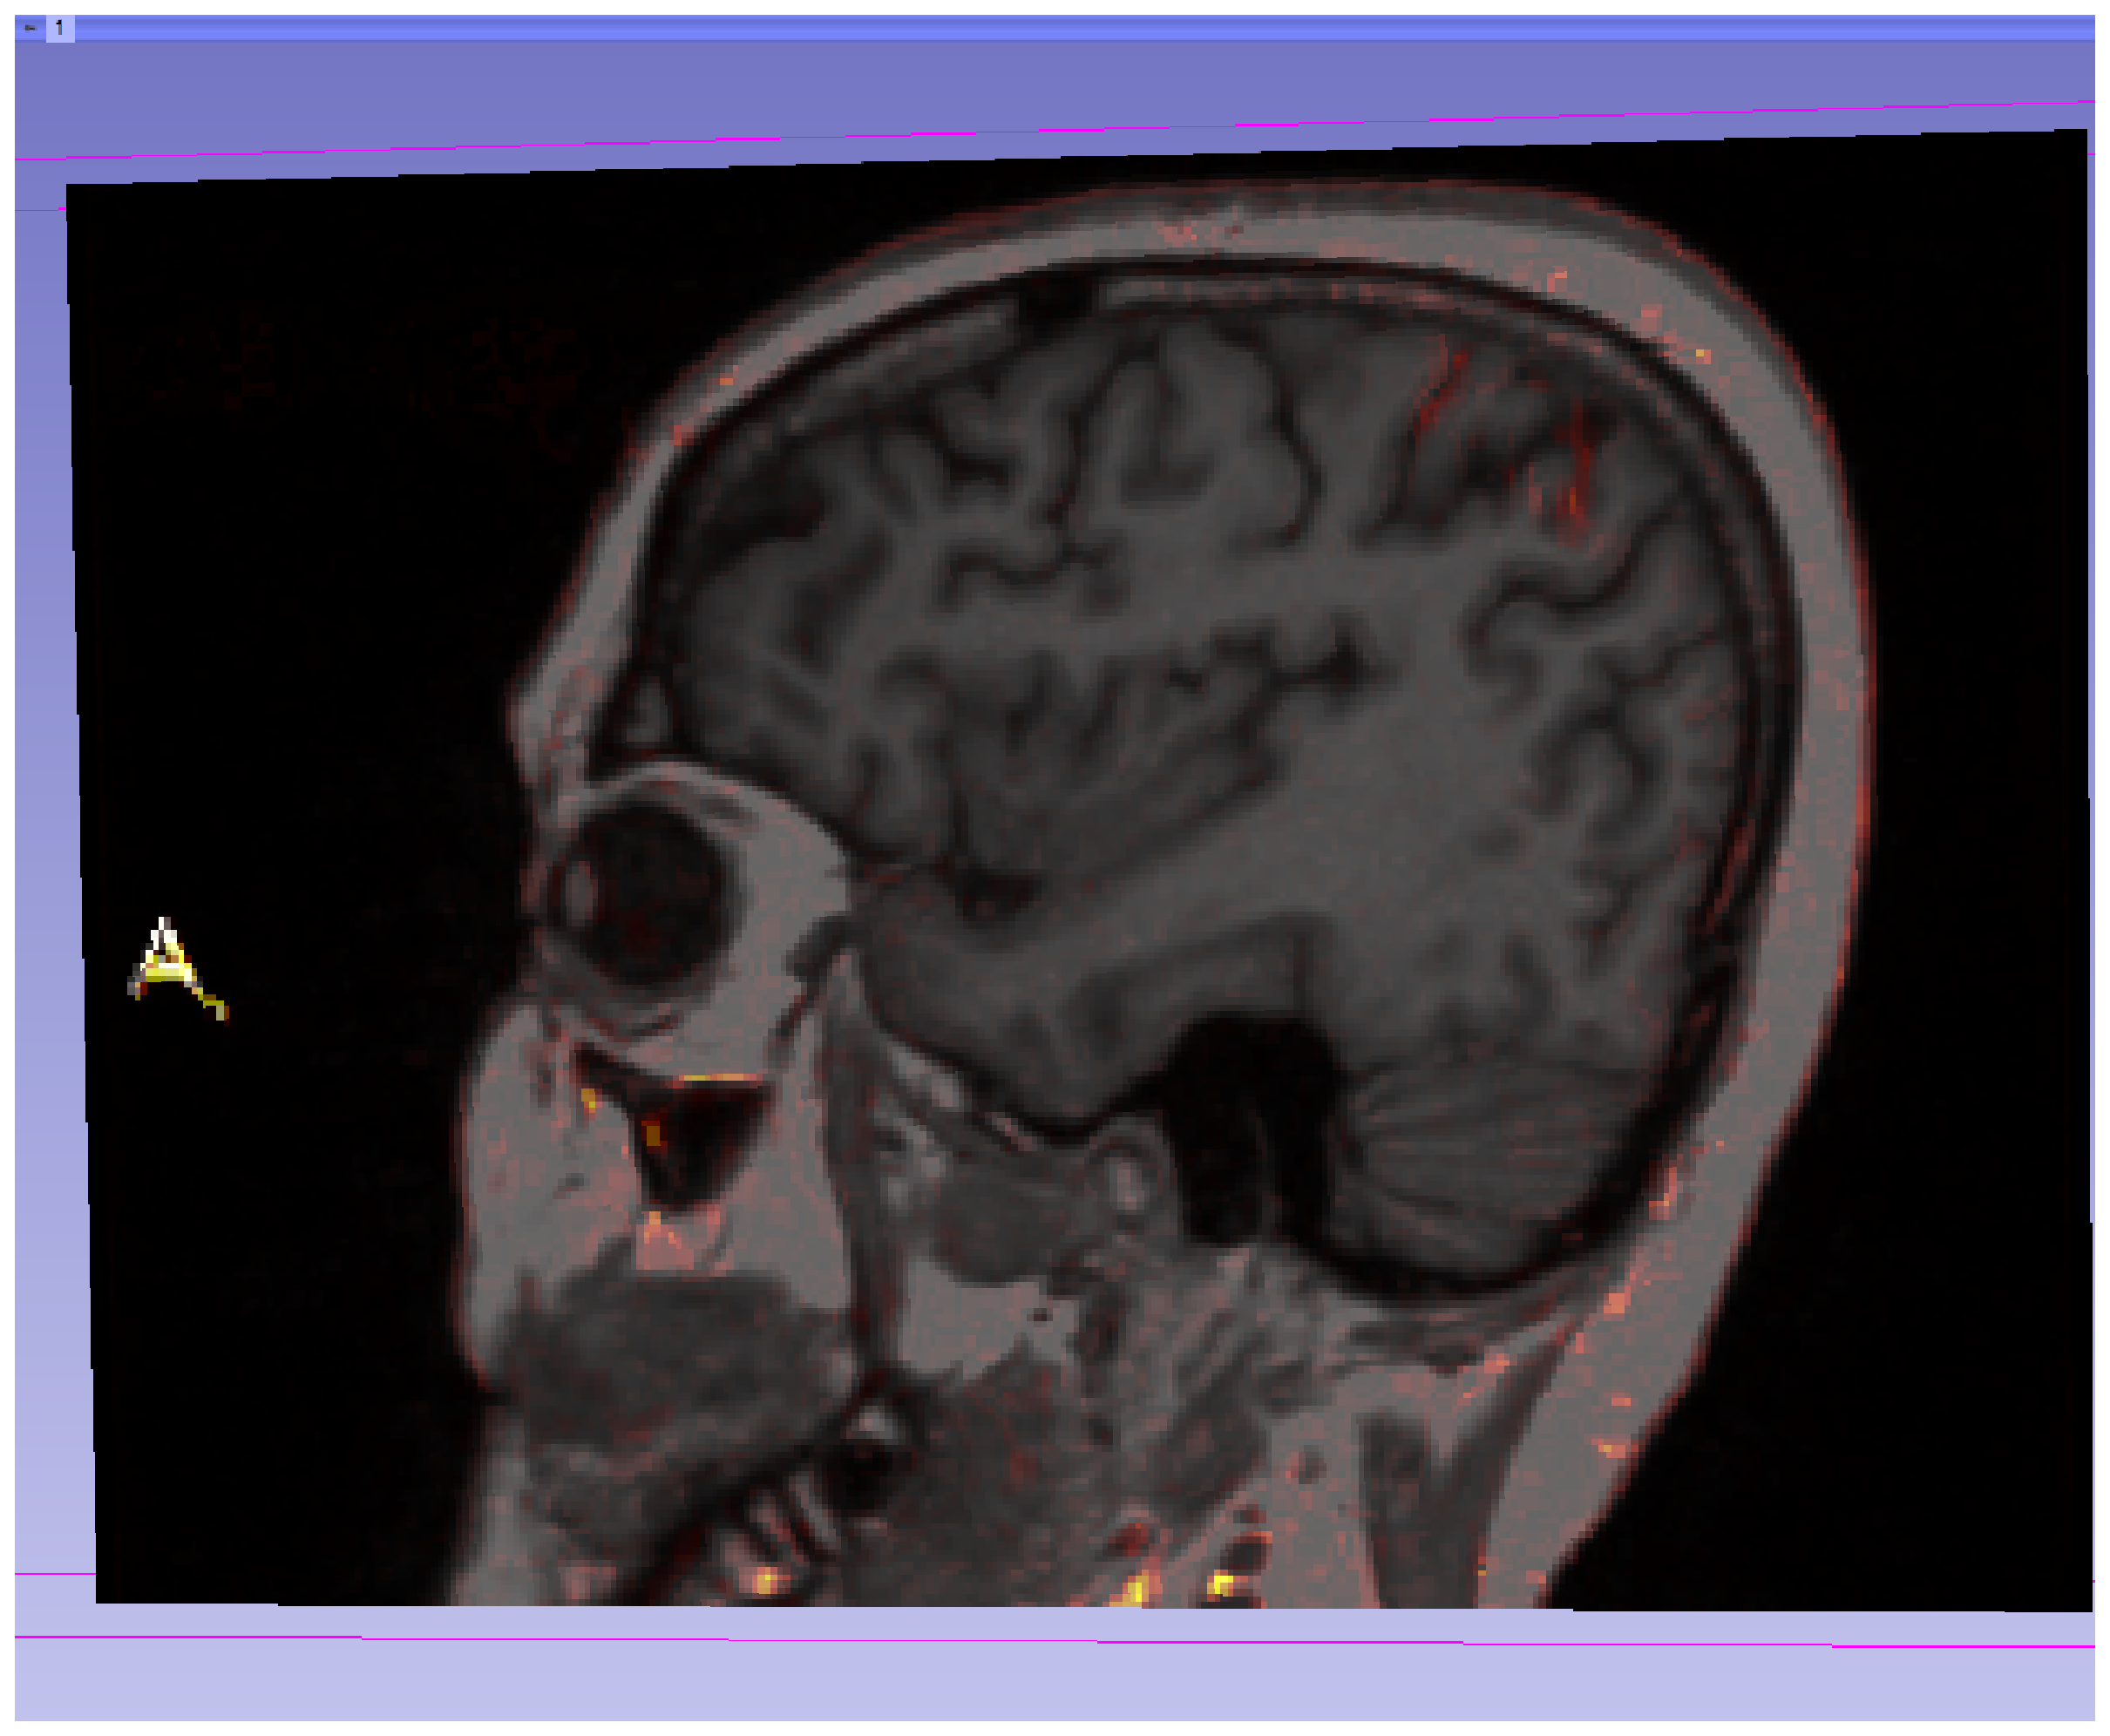
\includegraphics[scale=0.2]{/experiment_CL_P1/CL_Sagittal.eps}
  \caption{Voxel-based method. Patient 1: Sagittal plane}
  \label{CL_Sagittal}
\end{figure}


\subsubsection{Tensor-based Method}
Parameters used:
\begin{description}
\item \textit{Deformation field smoothing sigma:} 2.5
\item \textit{Shrinkage percentage:} 70
\item \textit{Growth percentage:} 75
\end{description}

\begin{figure}[H]
  \centering
  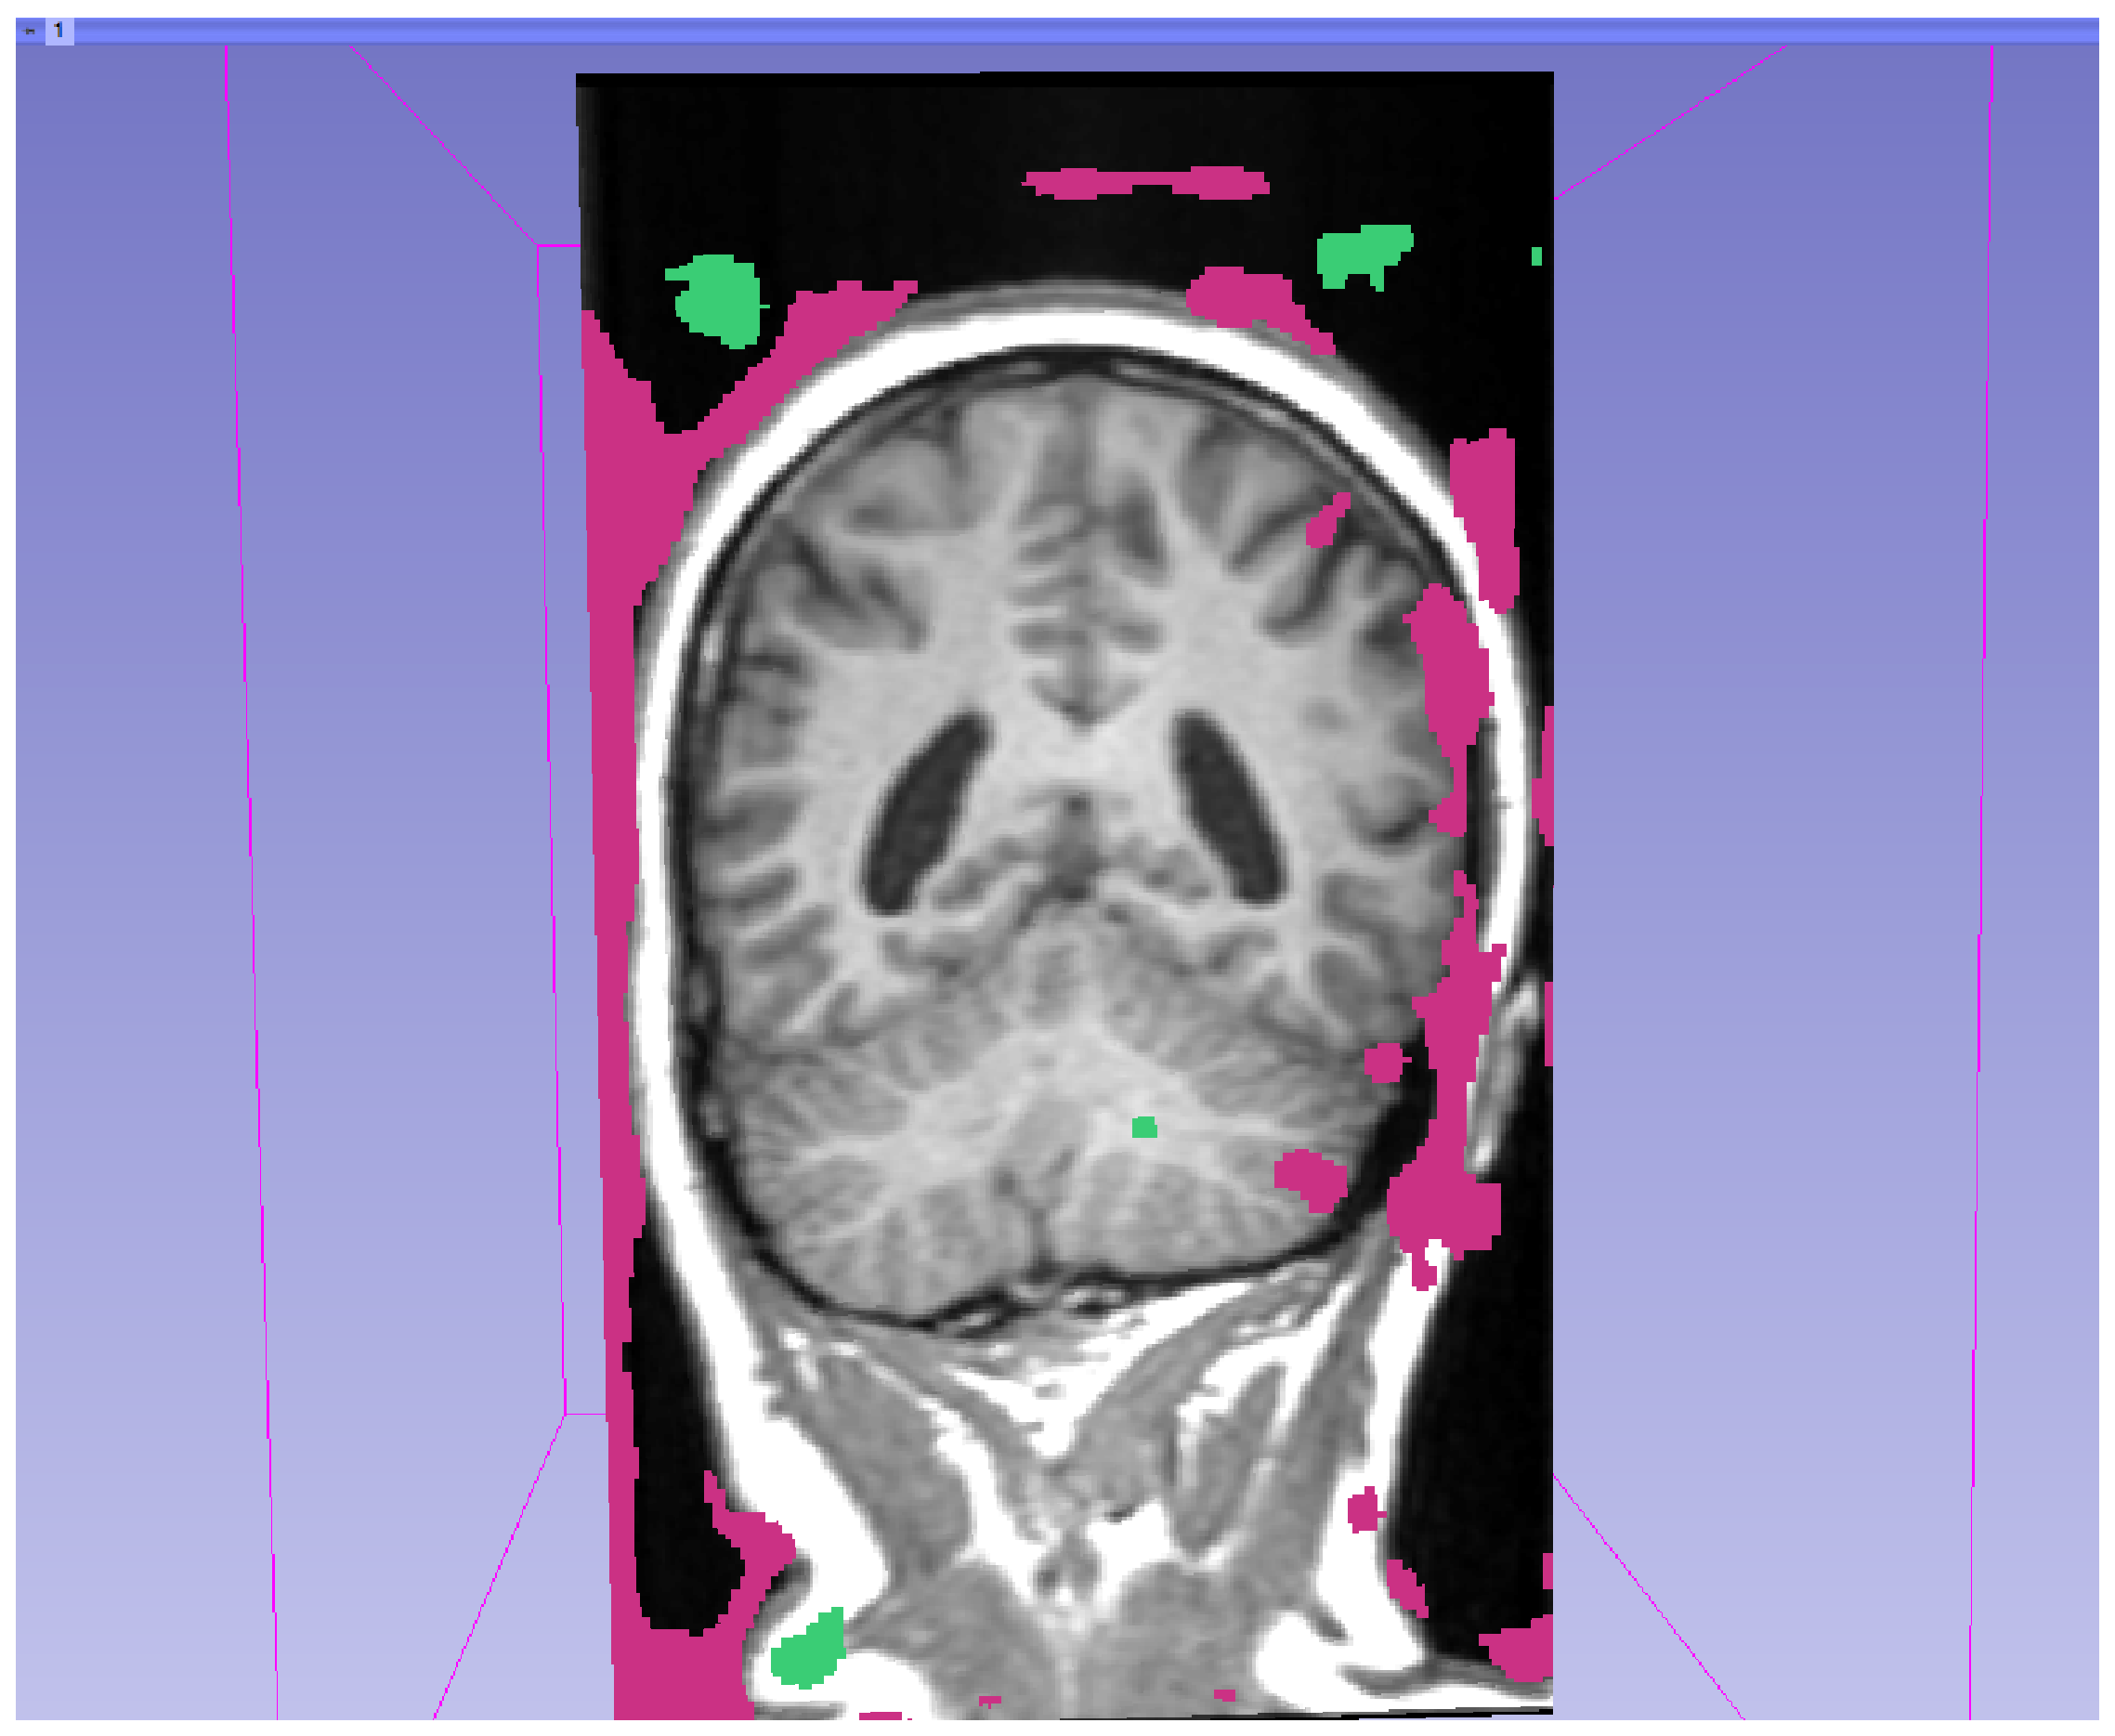
\includegraphics[scale=0.2]{/experiment_CL_P1/CL_Tensor_Coronal.eps}
  \caption{Tensor-based method. Patient 1: Coronal plane}
  \label{CL_TCoronal}
\end{figure}

\begin{figure}[H]
  \centering
  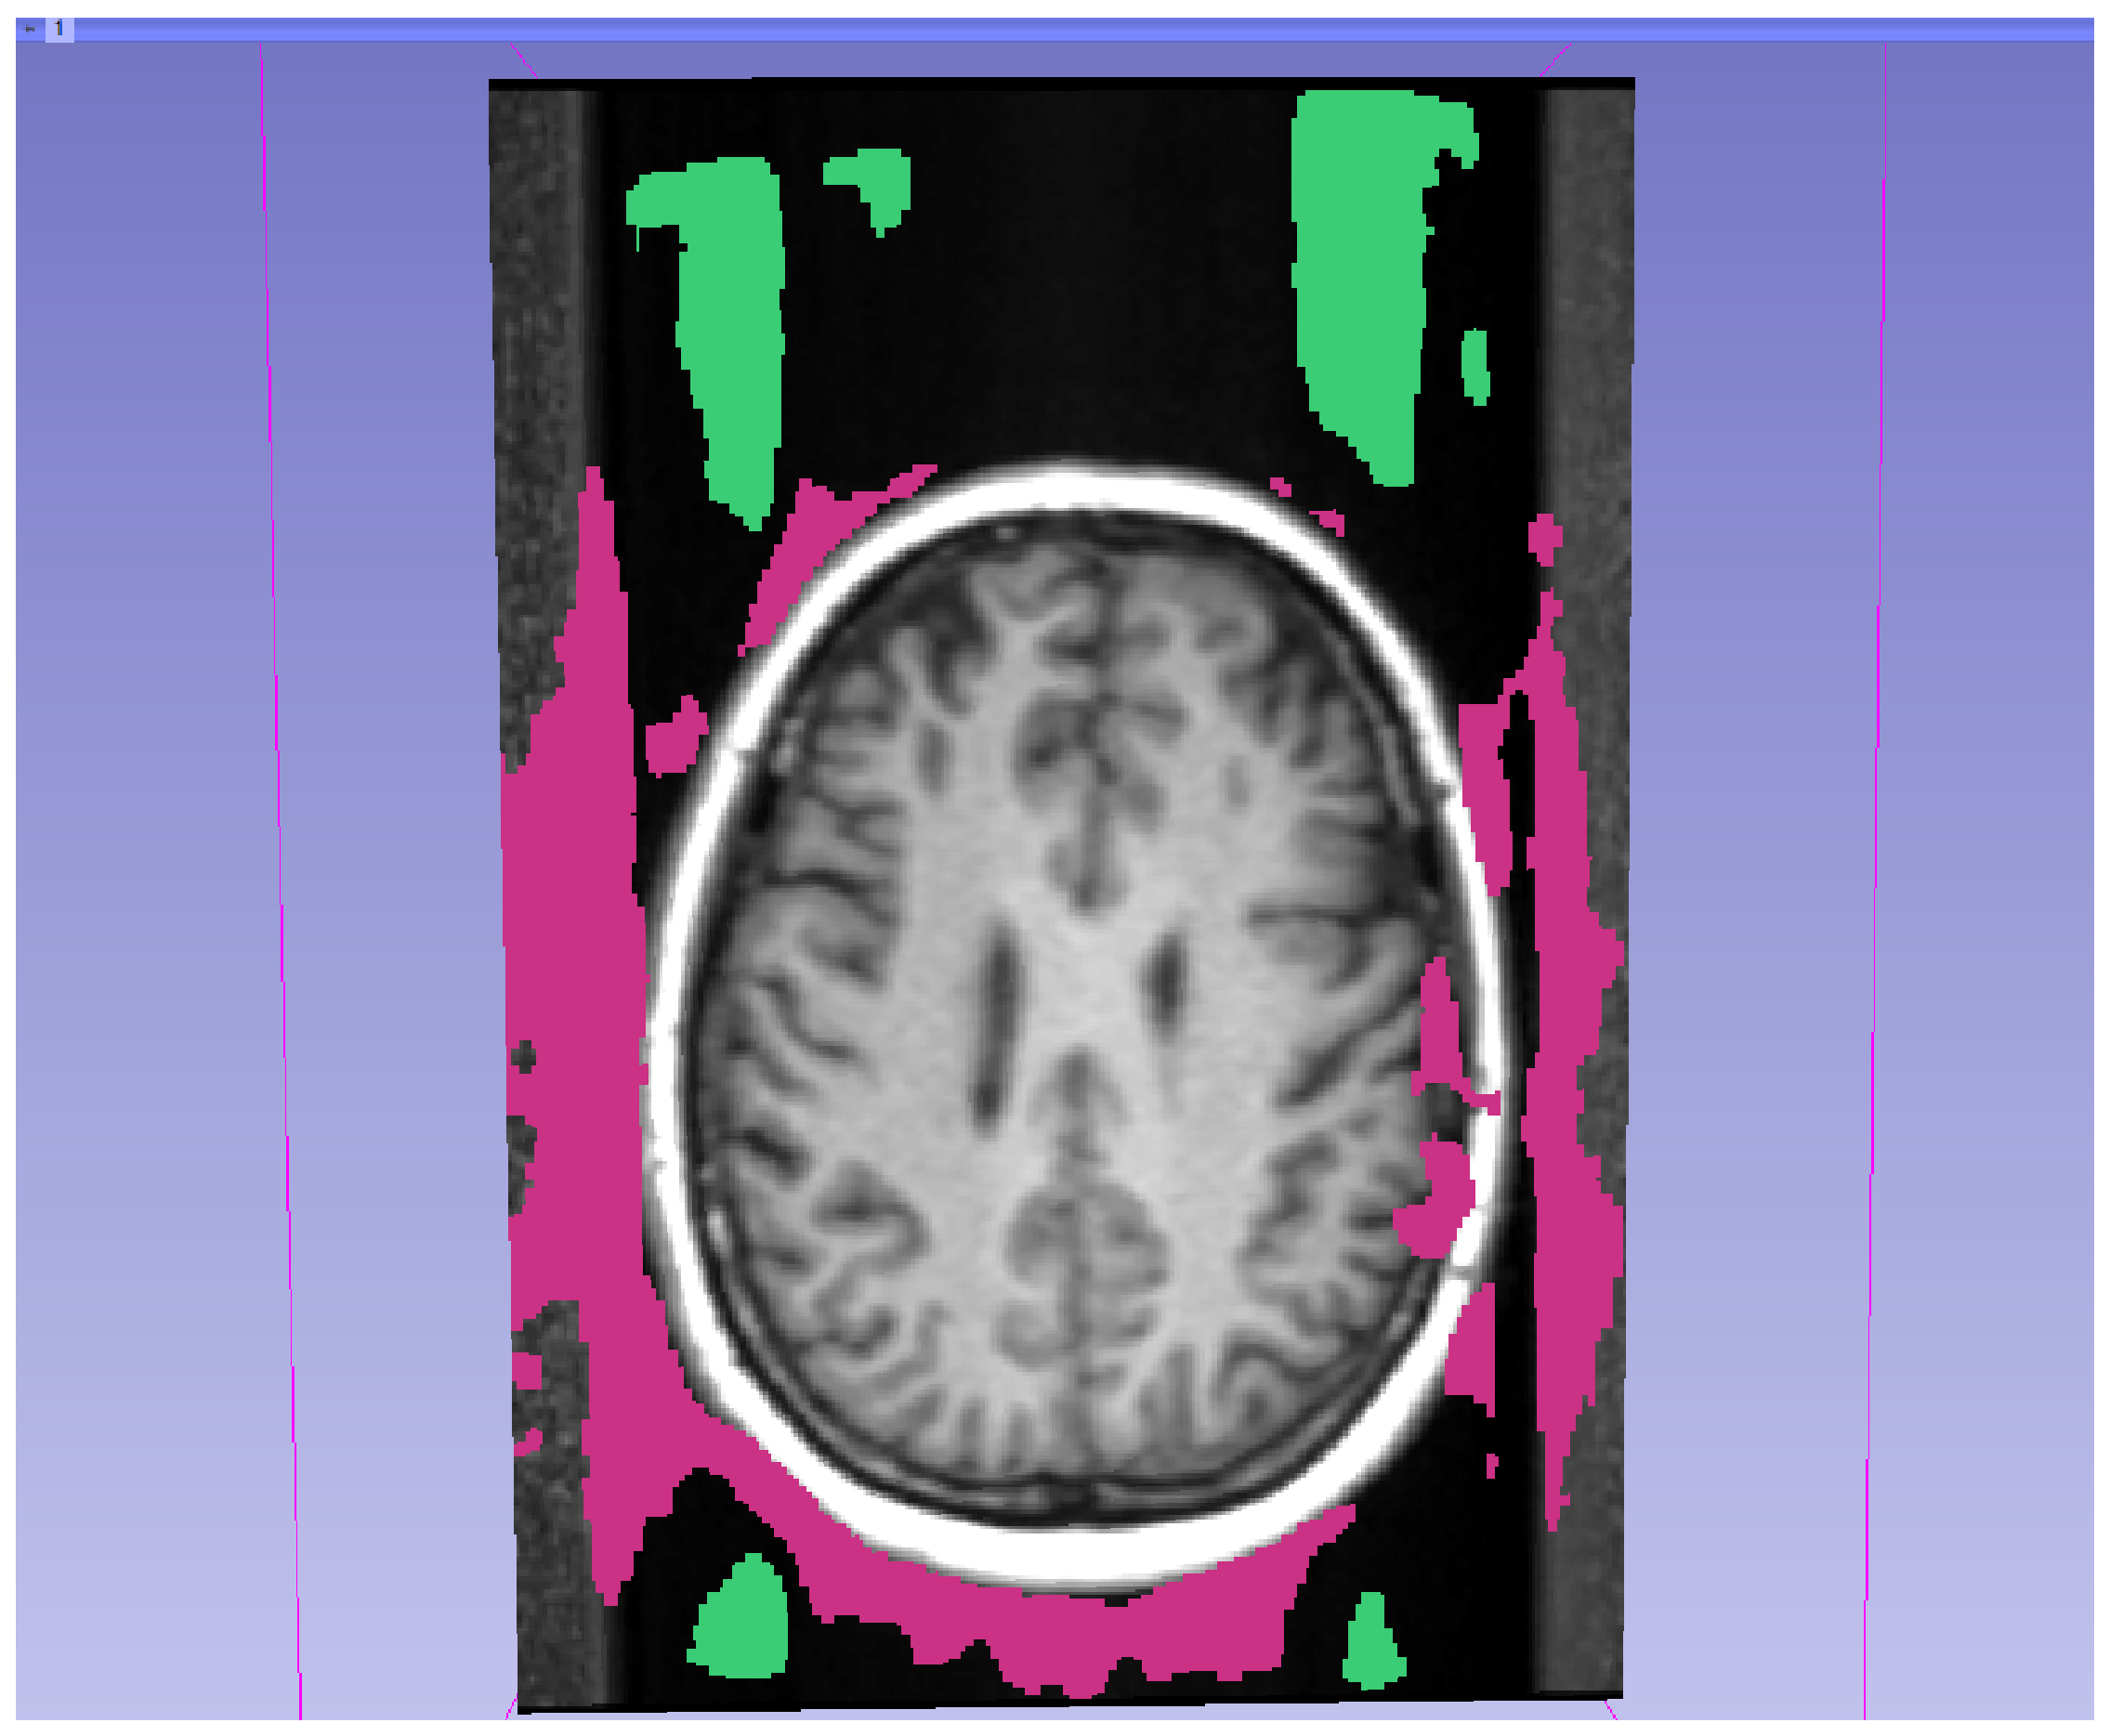
\includegraphics[scale=0.2]{/experiment_CL_P1/CL_Tensor_Traversal.eps}
  \caption{Tensor-based method. Patient 1: Traversal plane}
  \label{CL_TTraversal}
\end{figure}

\begin{figure}[H]
  \centering
  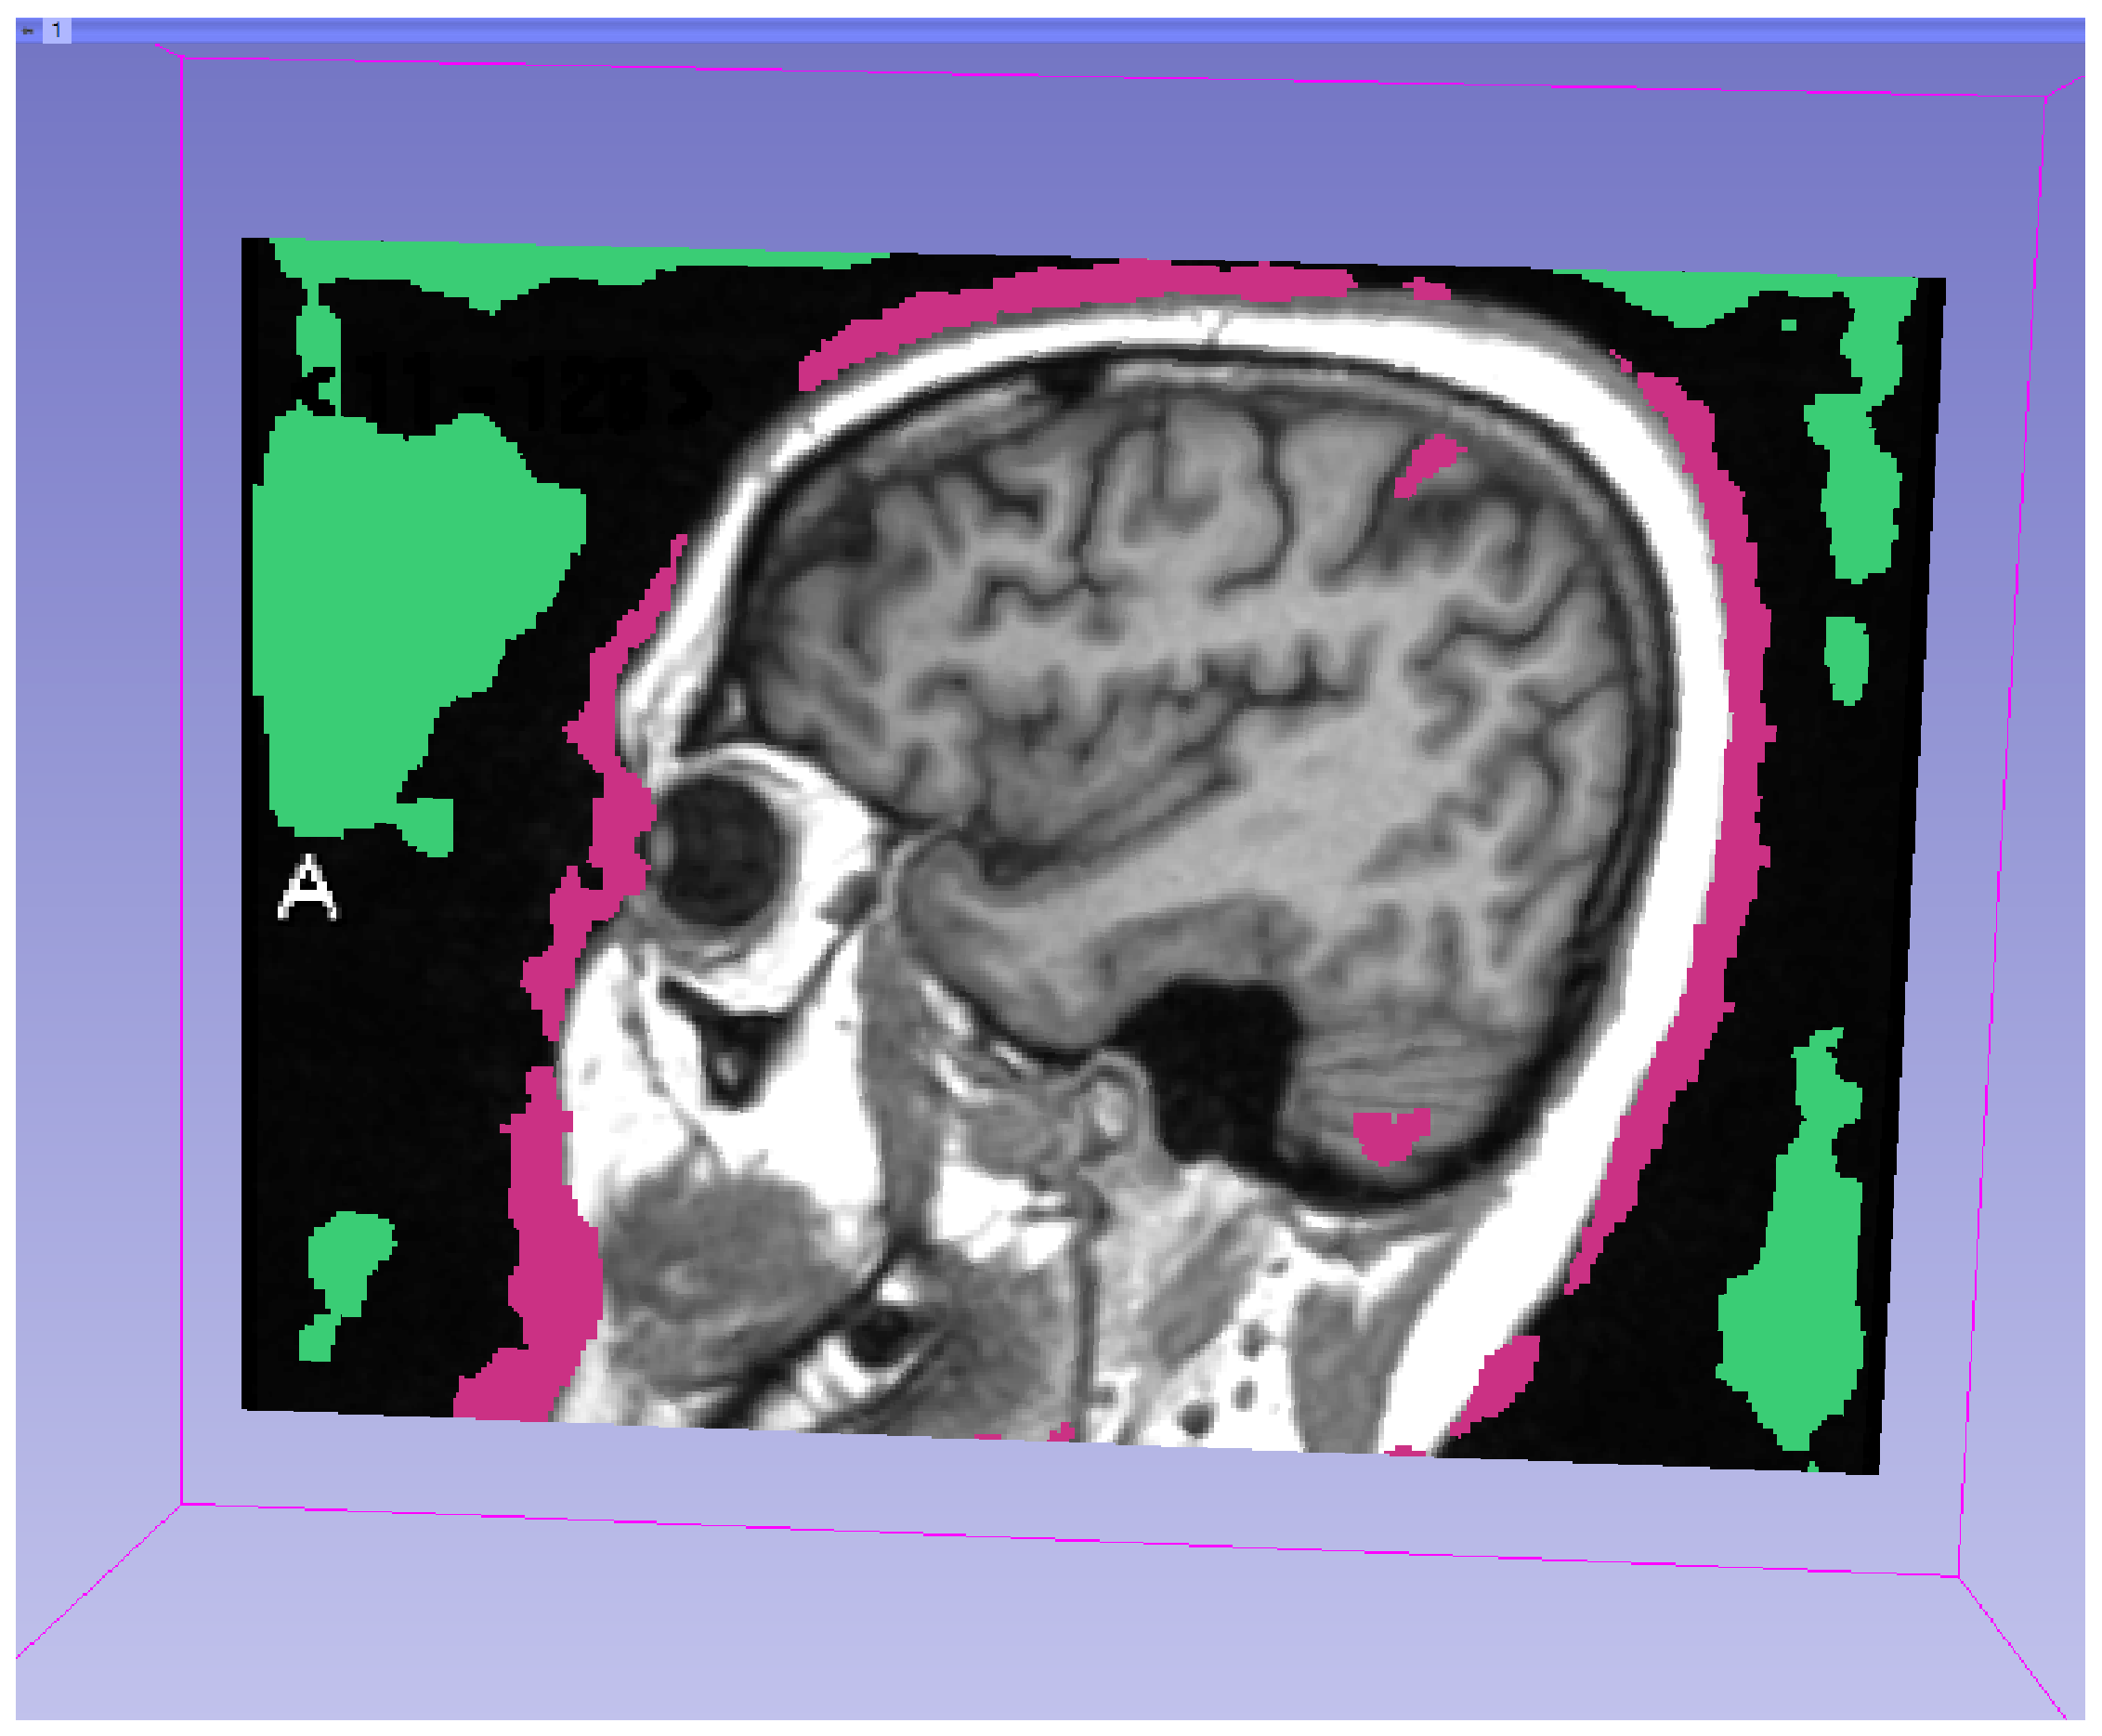
\includegraphics[scale=0.2]{/experiment_CL_P1/CL_Tensor_Sagittal.eps}
  \caption{Tensor-based method. Patient 1: Sagittal plane}
  \label{CL_TSagittal}
\end{figure}


\subsection{Patient 2}
The differences in this patient, if actually present, are really
small. 

\subsubsection{Voxel-based Method}
The voxel-based method shows small differences near the corpus
callosum on the three planes; this differences, accourding to the
medical expert, might be real because this is a very common area
affected by trauma.\\

The registration method used was \textit{Affine registration}.

\begin{figure}[H]
  \centering
  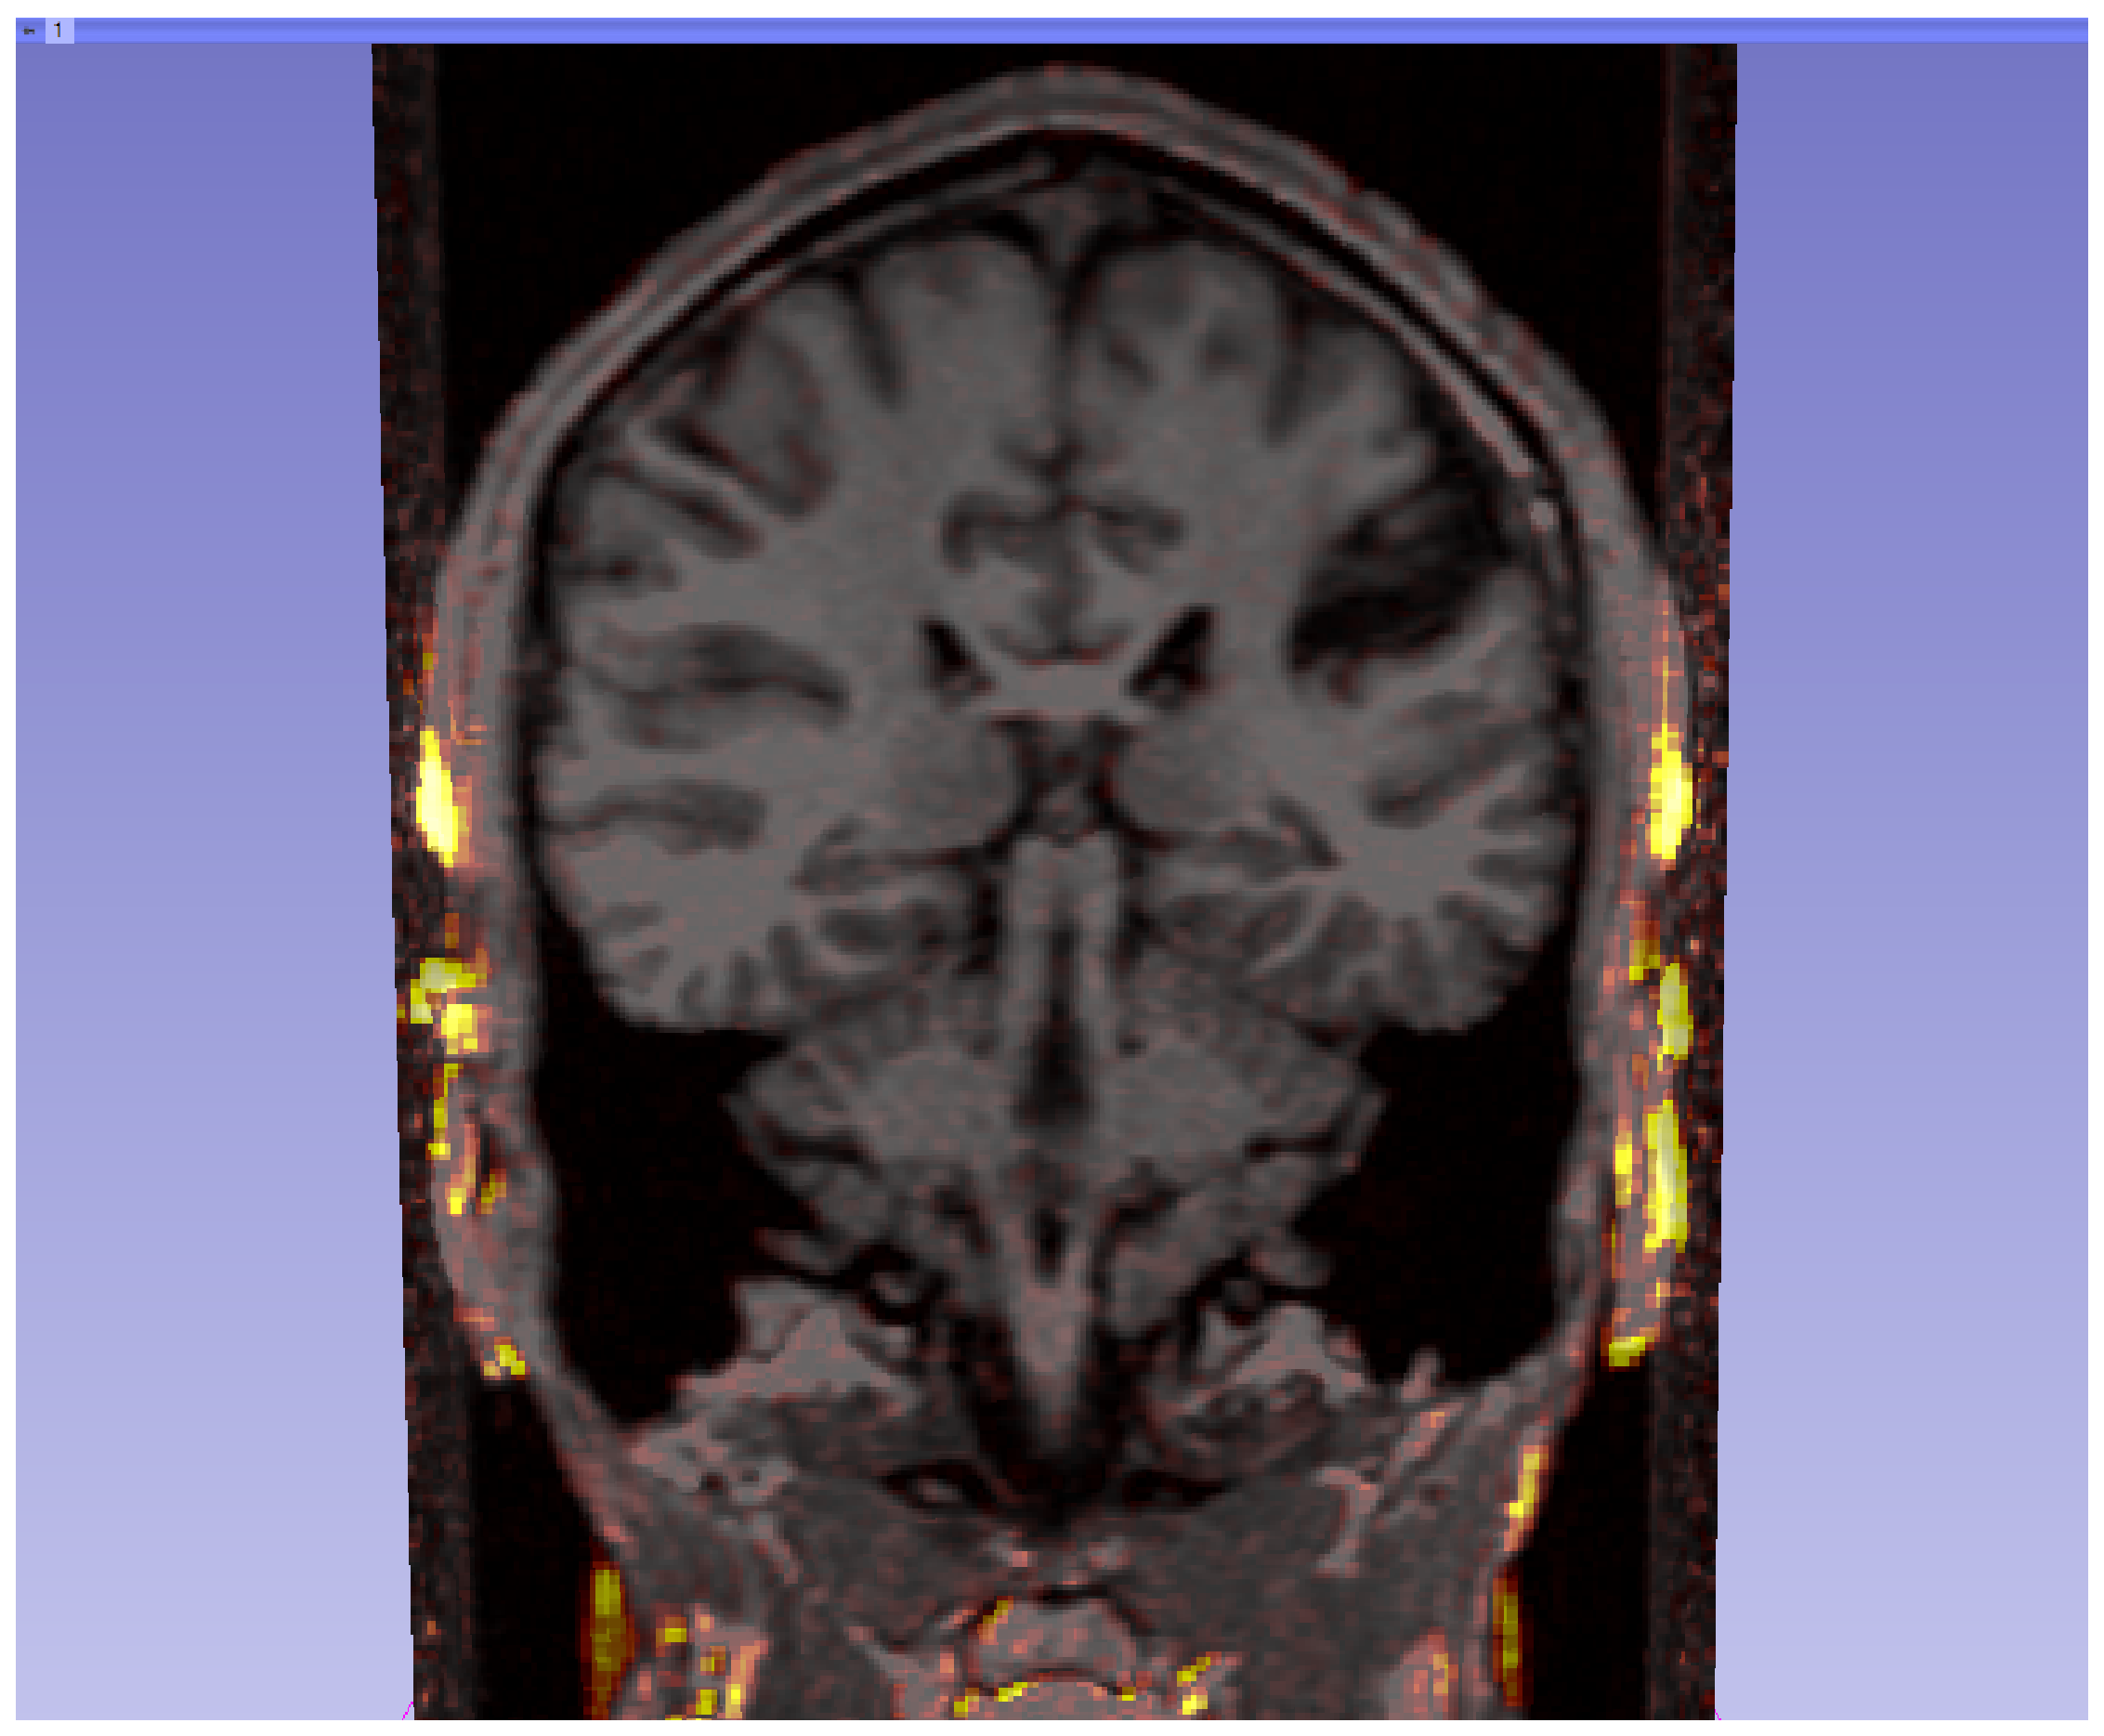
\includegraphics[scale=0.2]{/experiment_PB_P2/PB_Coronal.eps}
  \caption{Voxel-based method. Patient 2: Coronal plane}
  \label{PB_Coronal}
\end{figure}

\begin{figure}[H]
  \centering
  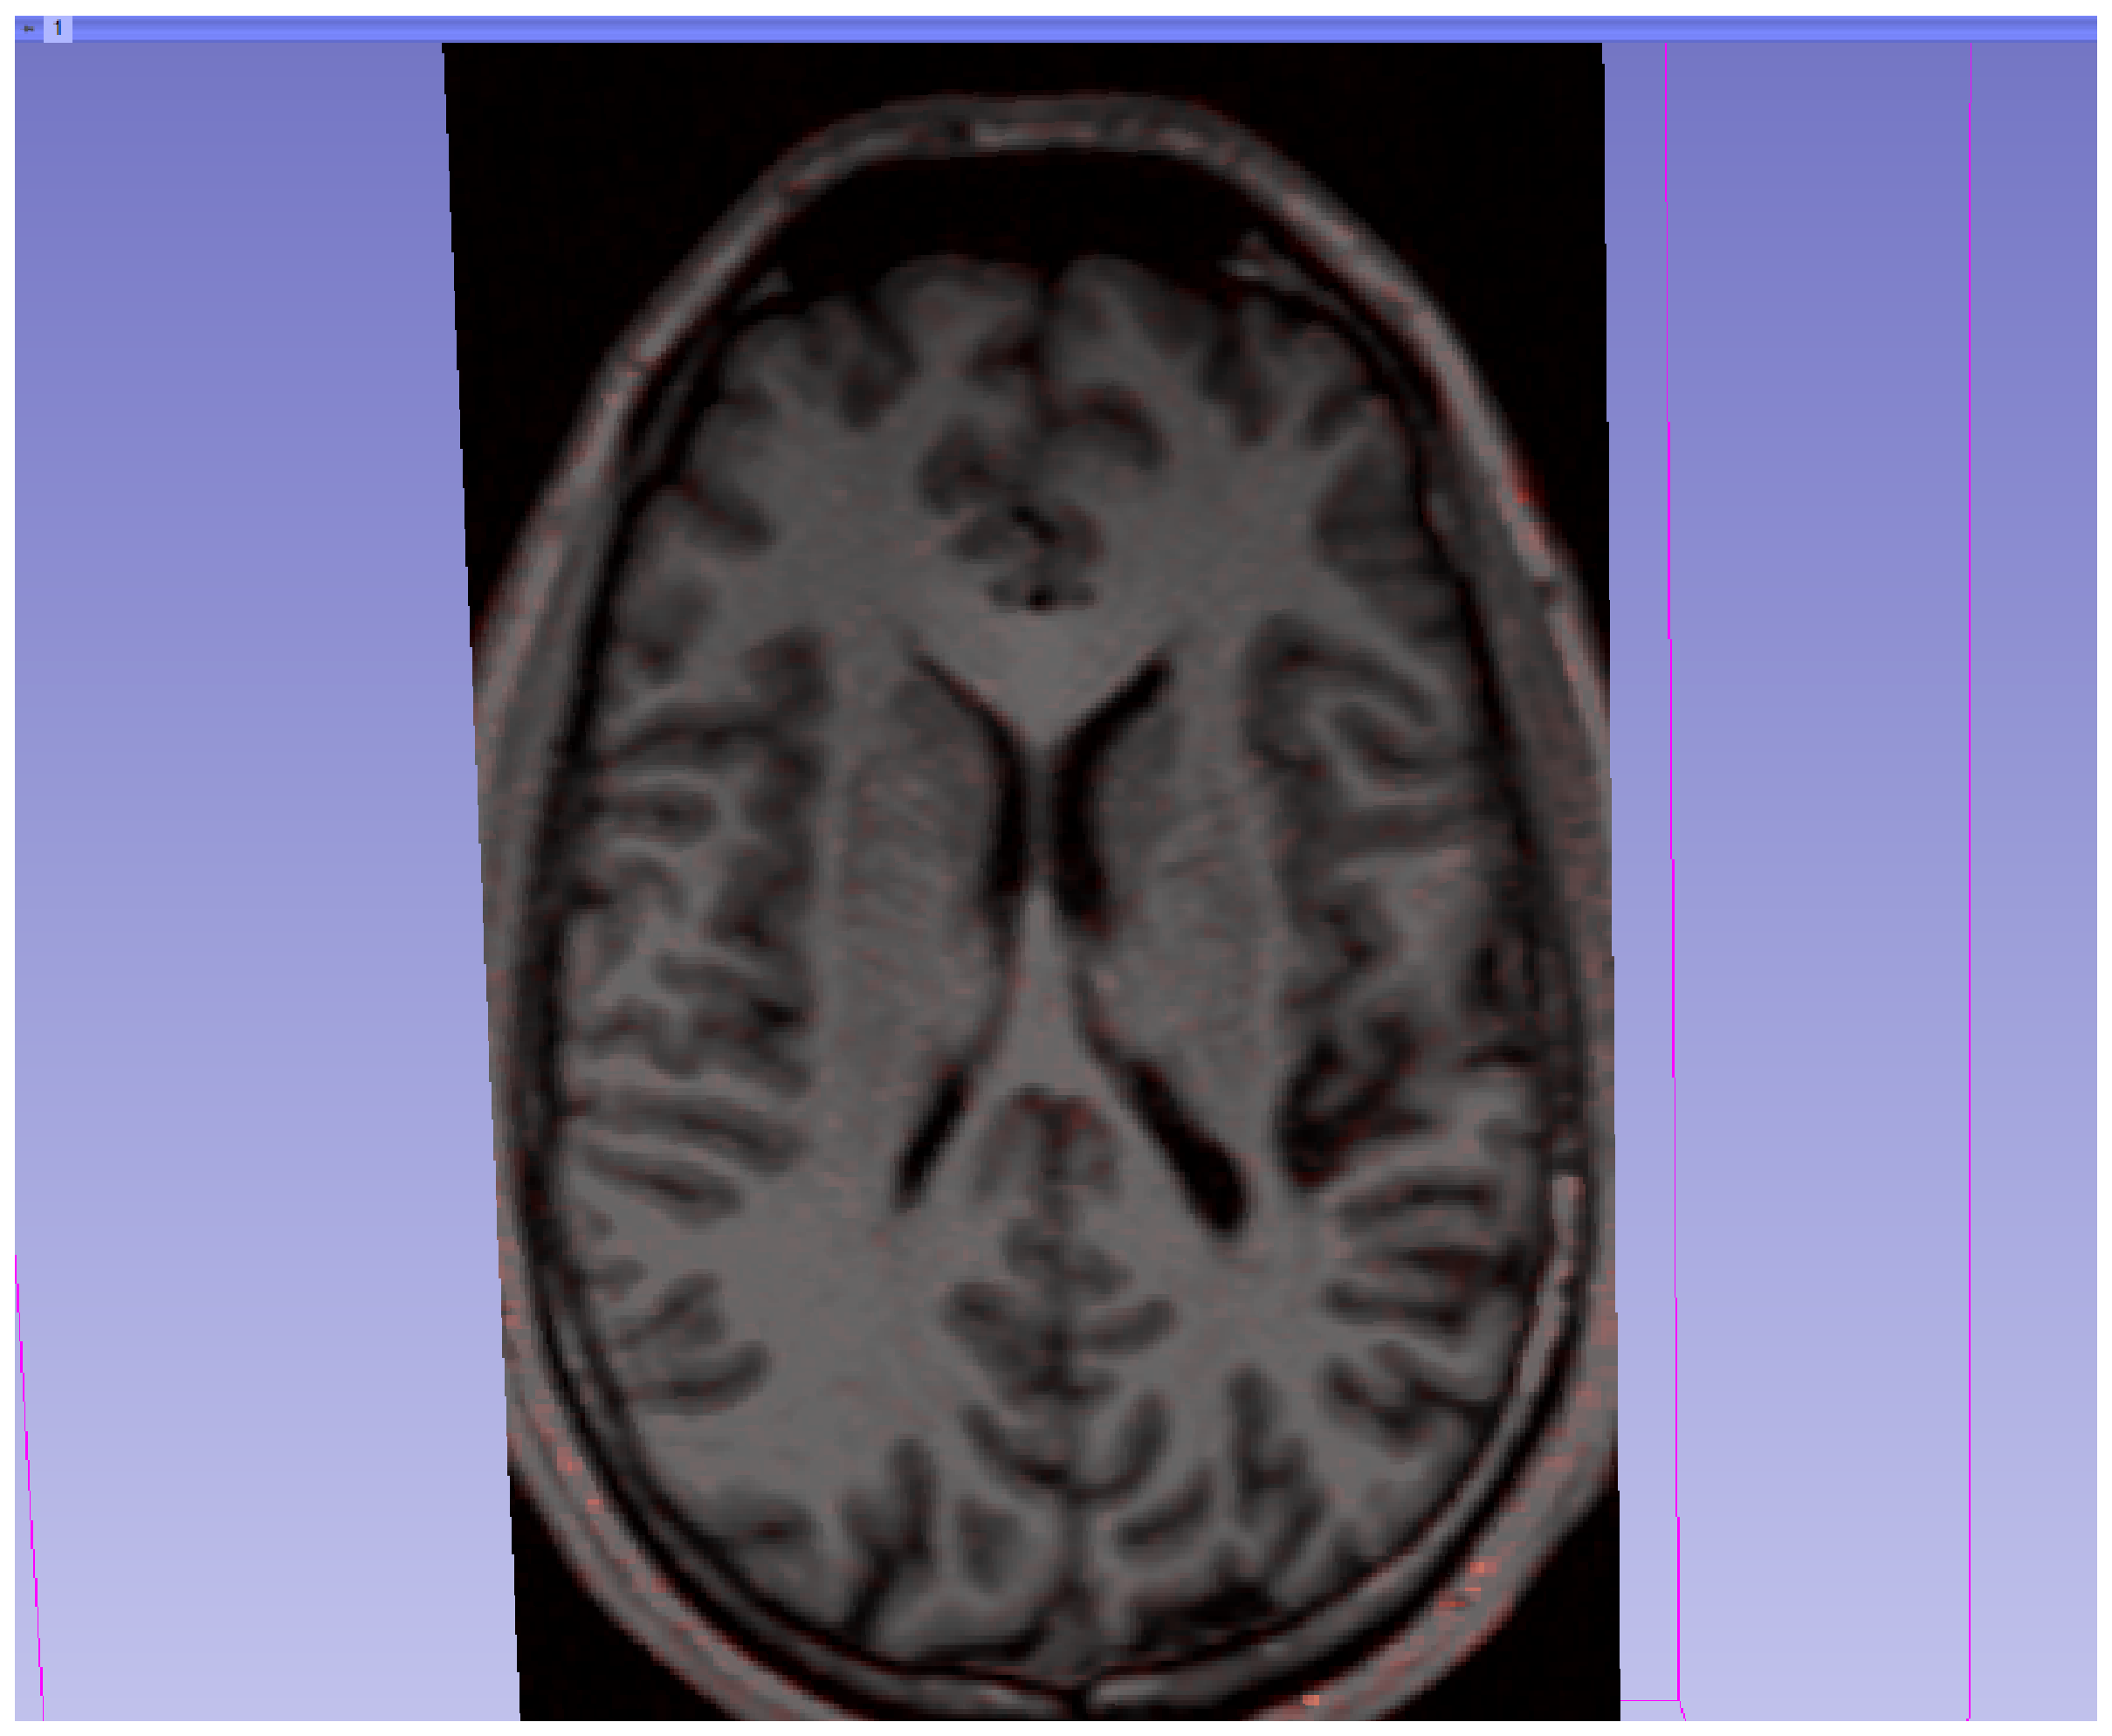
\includegraphics[scale=0.2]{/experiment_PB_P2/PB_Traversal.eps}
  \caption{Voxel-based method. Patient 2: Traversal plane}
  \label{PB_Traversal}
\end{figure}

\begin{figure}[H]
  \centering
  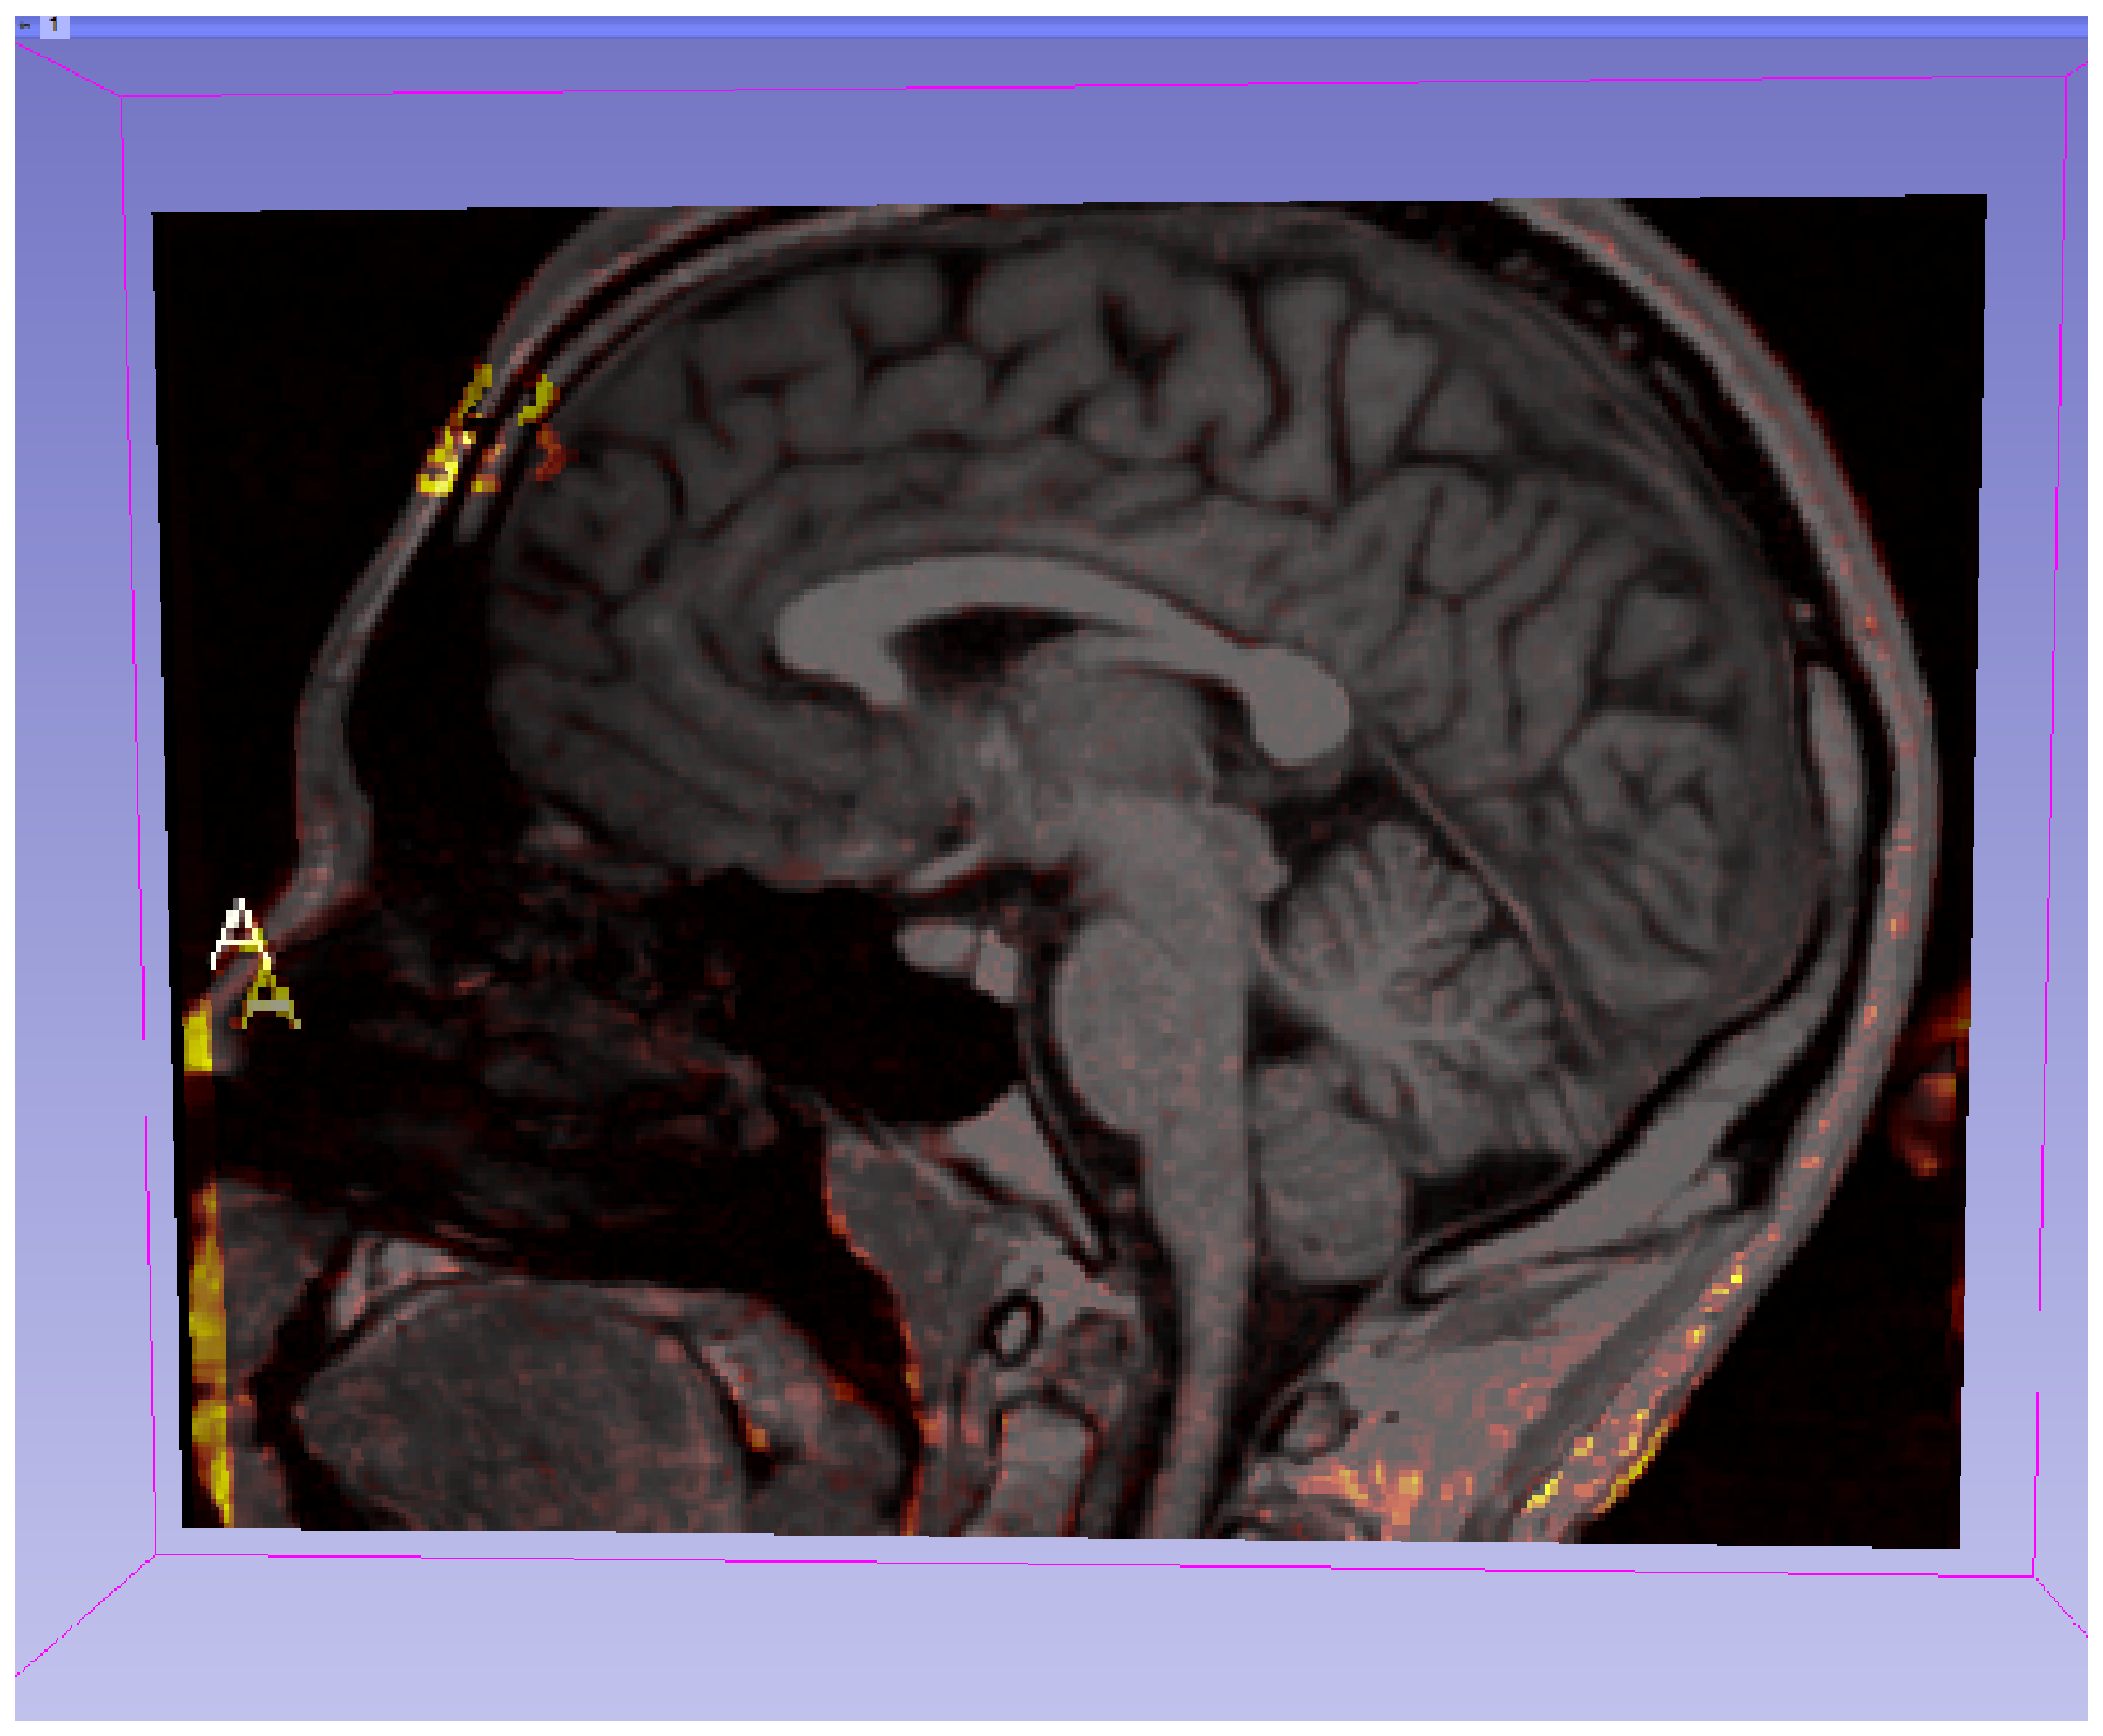
\includegraphics[scale=0.2]{/experiment_PB_P2/PB_Sagittal.eps}
  \caption{Voxel-based method. Patient 2: Sagittal plane}
  \label{PB_Sagittal}
\end{figure}


\subsubsection{Tensor-based Method}
The tensor-base method doesn't find the same differences in the corpus
callosum as the previous method. With the usual percentage values
(from $70\%$ to $80\%$ for both growth and shrinkage), the method almost
doesn't find any differences. 

In order to show some of the possible places where the method shows
some type of differences, the value of the shrinkage percentage was
increased until $88\%$. Given this, the pink areas shown are not
necessarily real differences.\\

Parameters used:
\begin{description}
\item \textit{Deformation field smoothing sigma:} 2.5
\item \textit{Shrinkage percentage:} 80
\item \textit{Growth percentage:} 88
\end{description}

\begin{figure}[H]
  \centering
  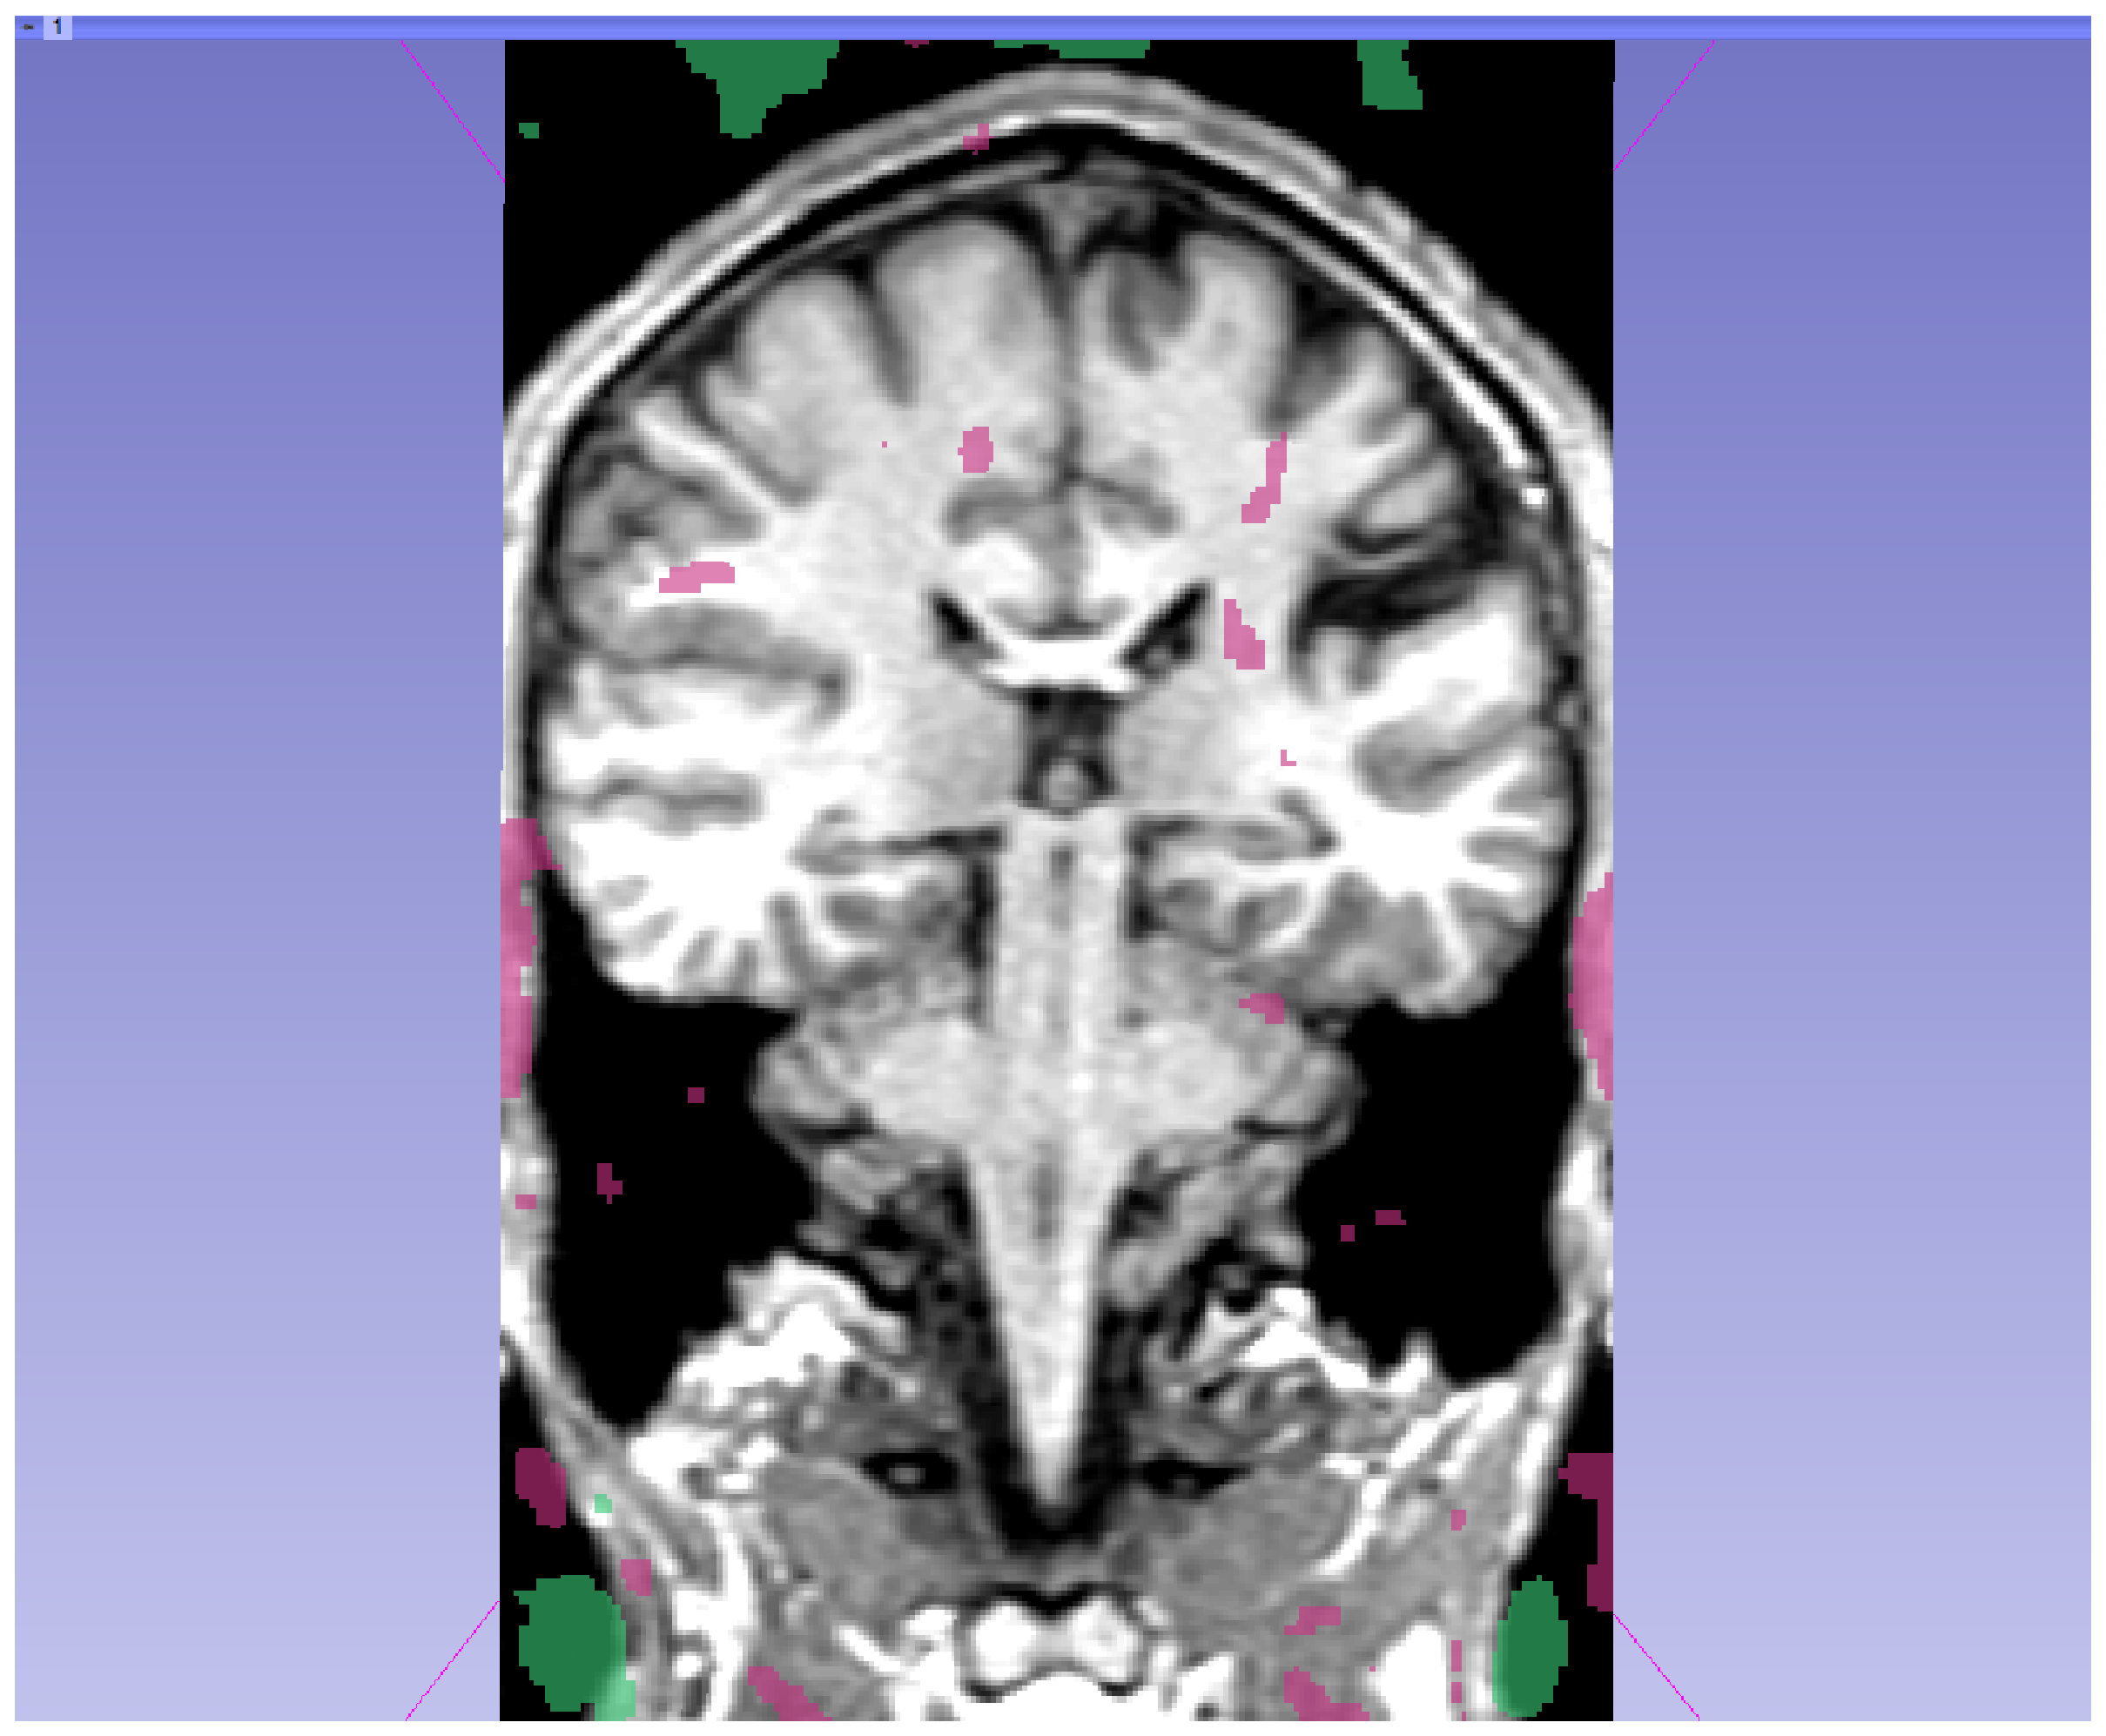
\includegraphics[scale=0.2]{/experiment_PB_P2/PB_Tensor_Coronal.eps}
  \caption{Tensor-based method. Patient 2: Coronal plane}
  \label{PB_TCoronal}
\end{figure}

\begin{figure}[H]
  \centering
  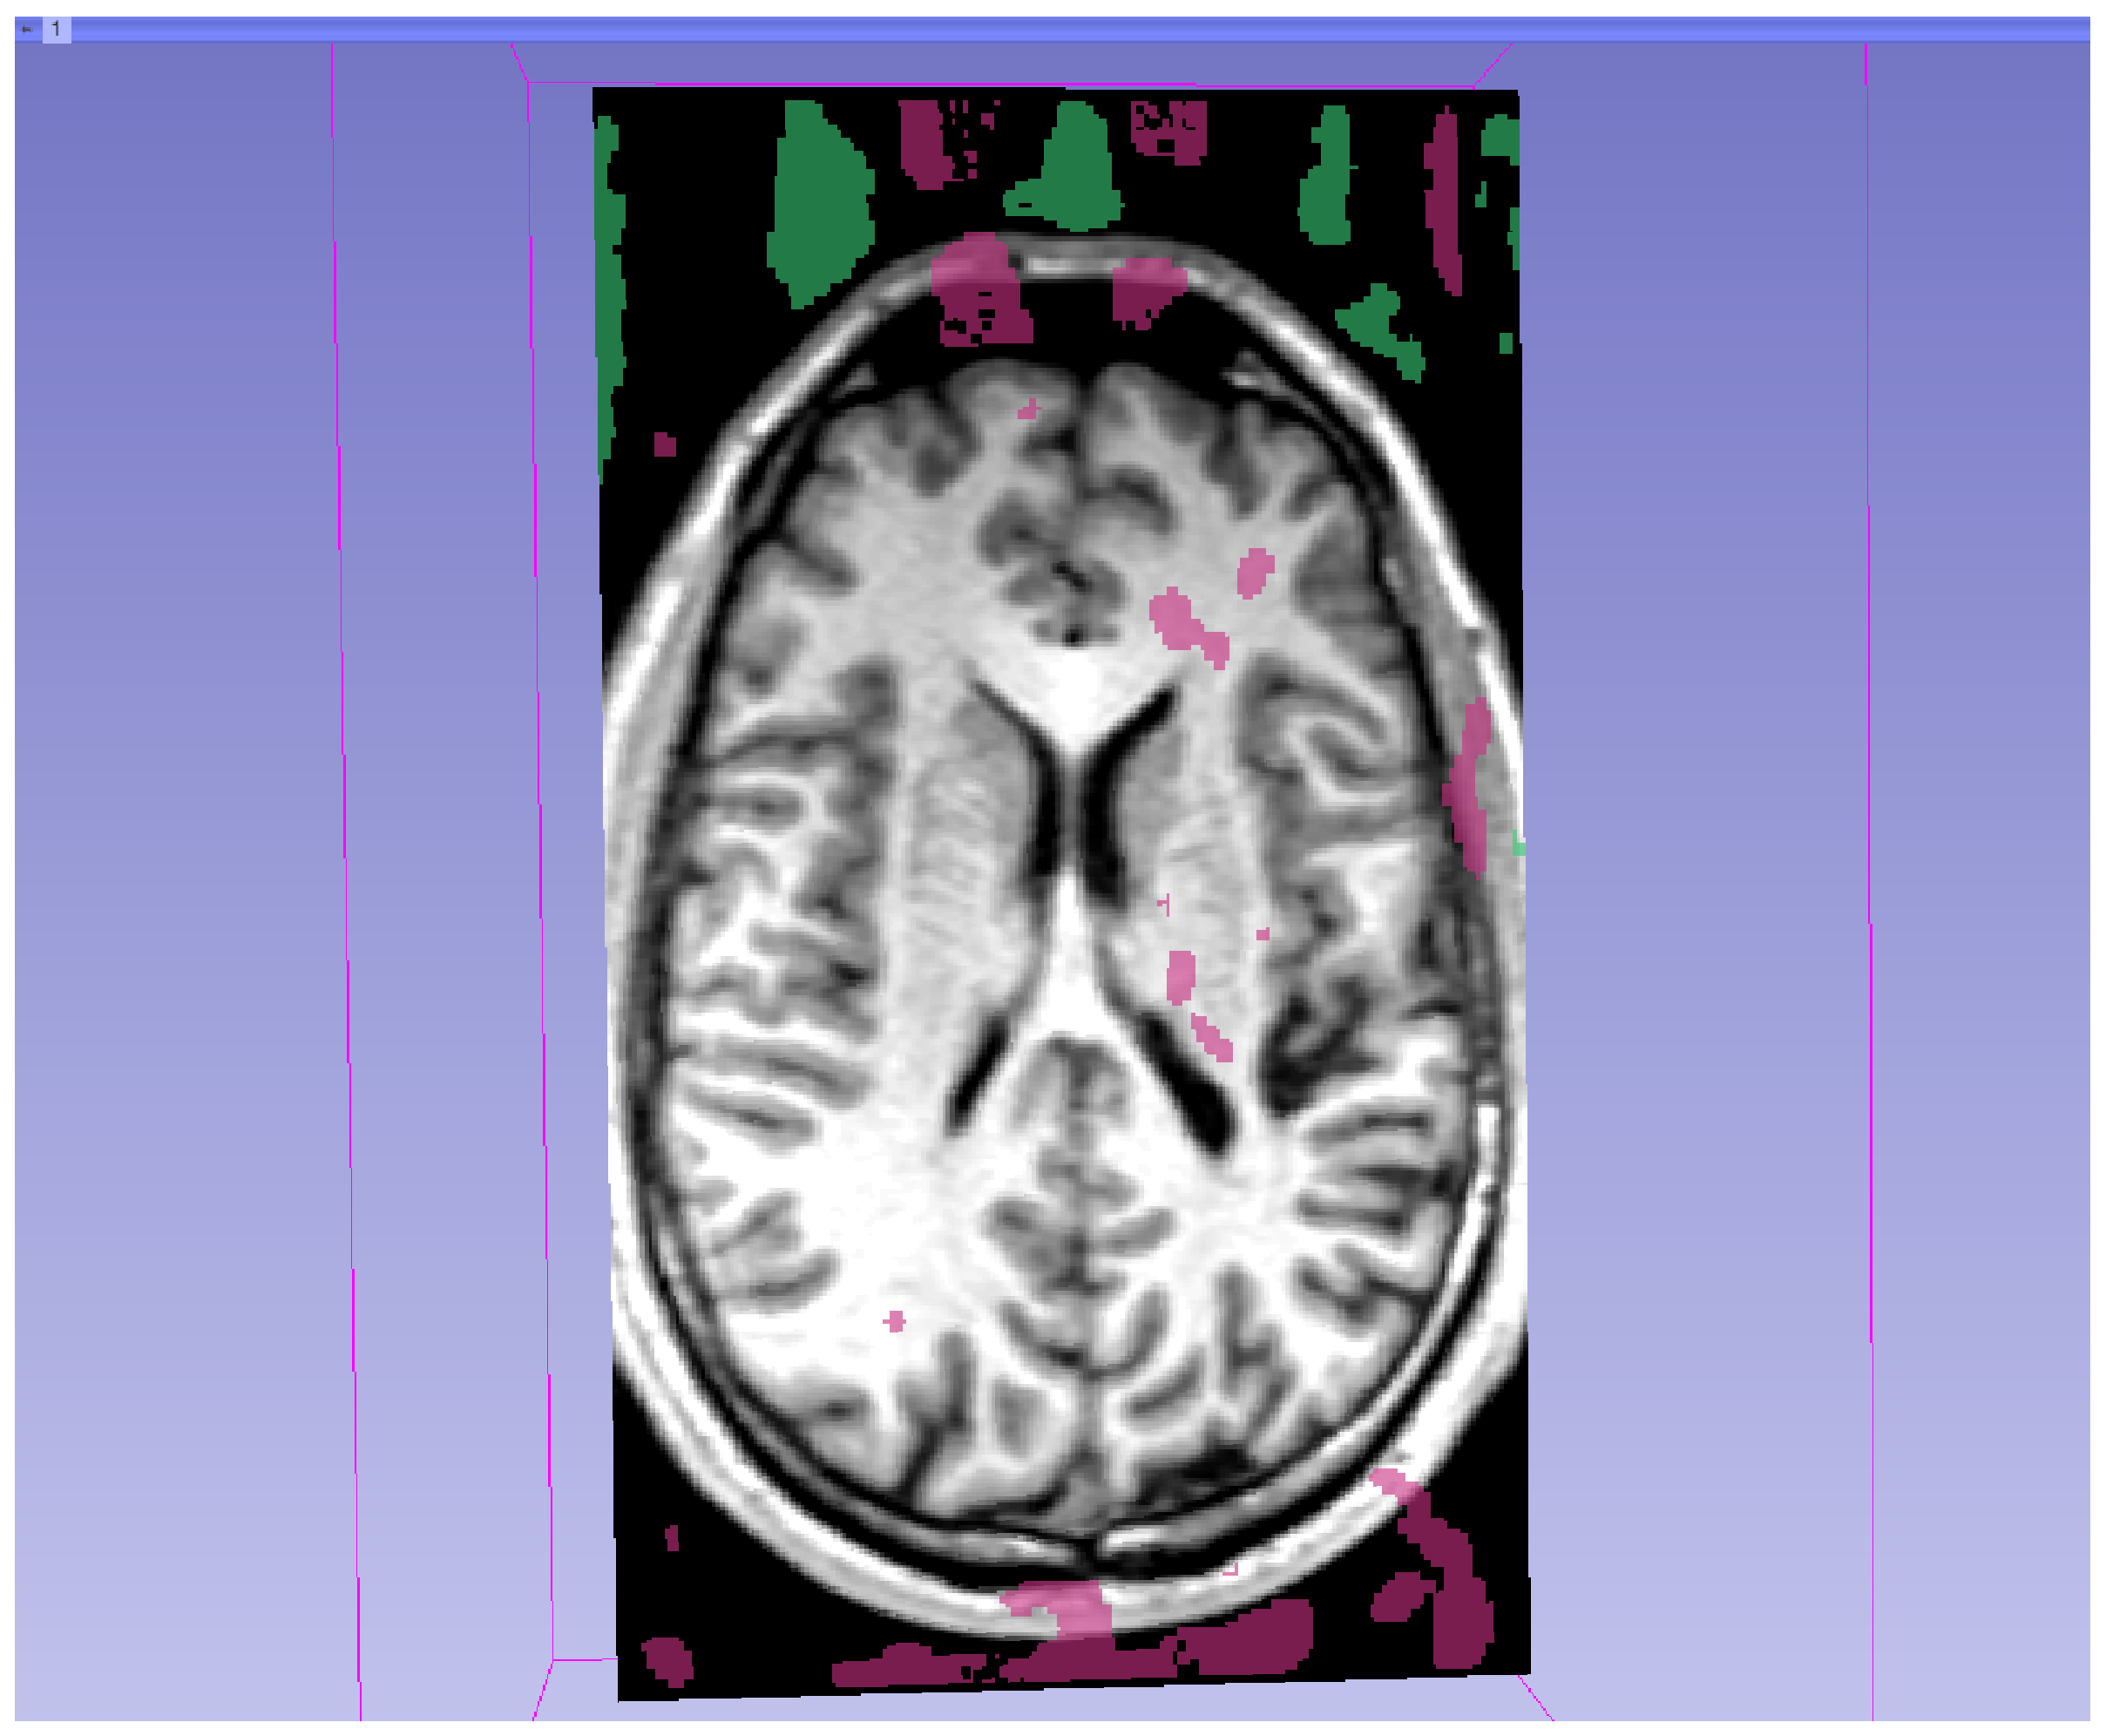
\includegraphics[scale=0.2]{/experiment_PB_P2/PB_Tensor_Traversal.eps}
  \caption{Tensor-based method. Patient 2: Traversal plane}
  \label{PB_TTraversal}
\end{figure}

\begin{figure}[H]
  \centering
  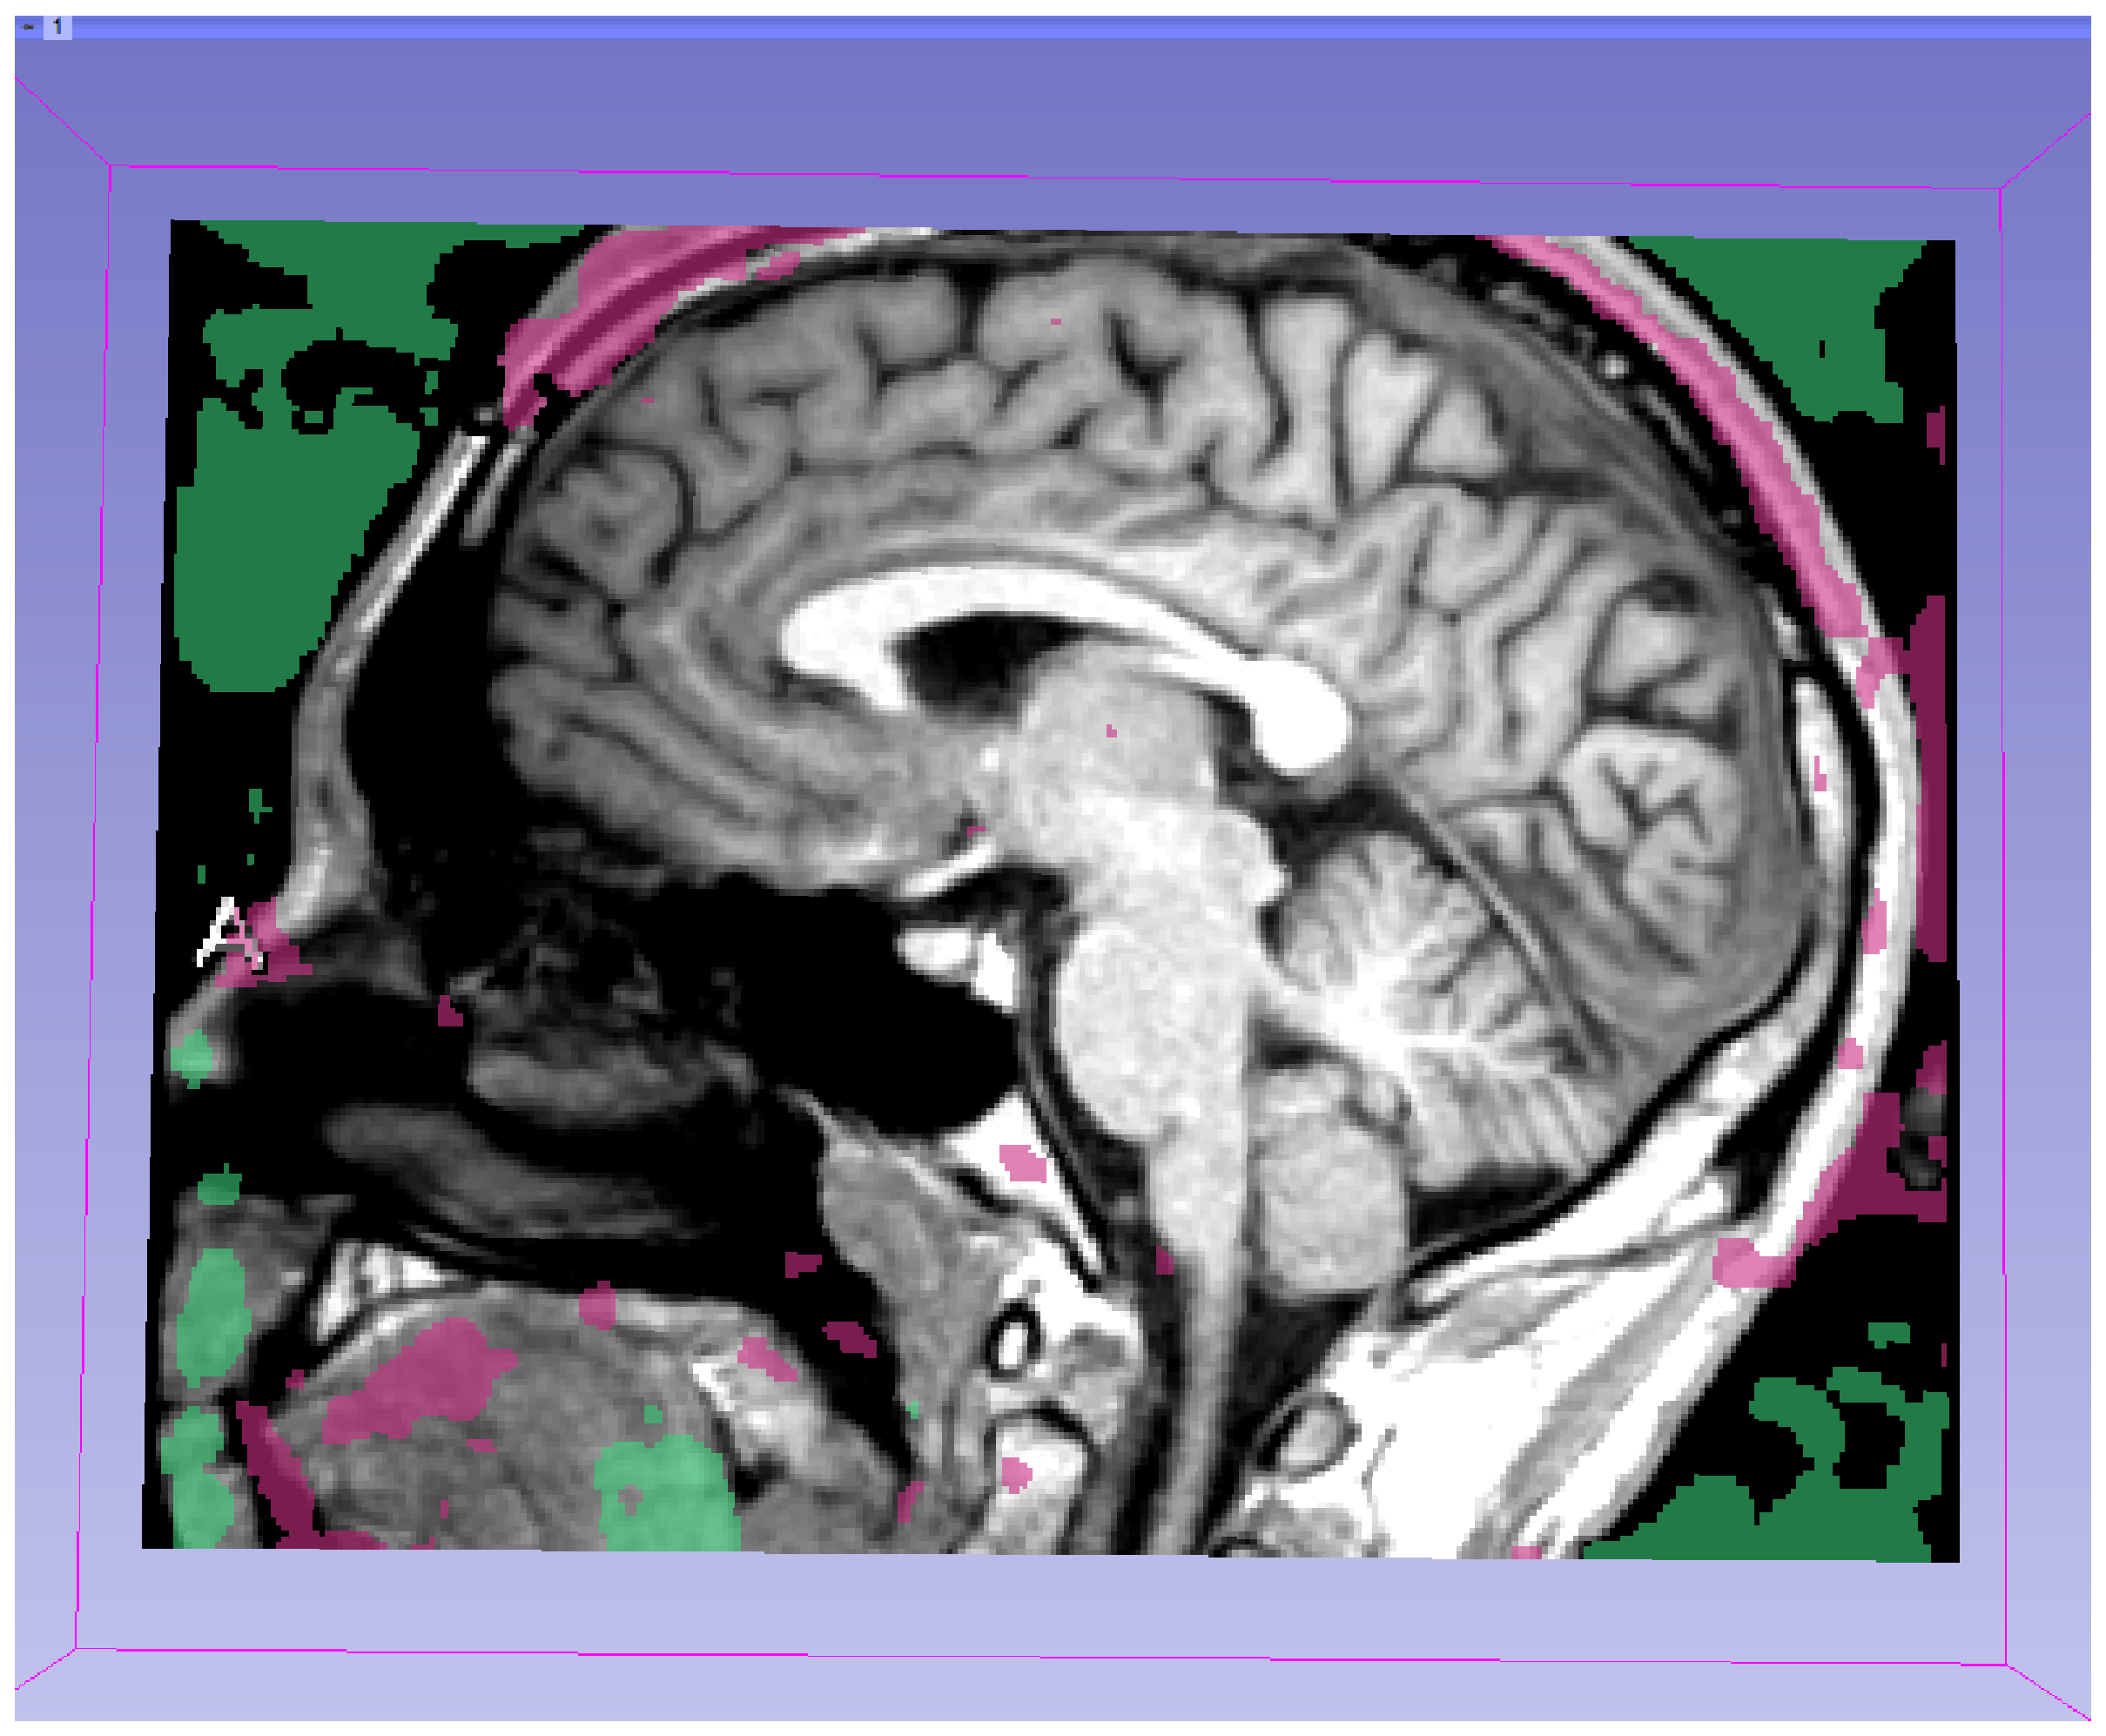
\includegraphics[scale=0.2]{/experiment_PB_P2/PB_Tensor_Sagittal.eps}
  \caption{Tensor-based method. Patient 2: Sagittal plane}
  \label{PB_TSagittal}
\end{figure}


\subsection{Patient 3}
This patient had a medical condition for which it has had two
surgeries performed. A tumor, located on the right hemisphere of the
frontal lobe, was removed during the first surgery. The MRIs used
during this experiment were taken before and after the second surgery,
in which a second growth was removed located the same area.


\subsubsection{Voxel-based Method}
The method shows the expected differences in the right hemisphere of
the frontal lobe of the brain. It also shows some size differences
especially in the lower parietal lobe, which can be observed in image
\ref{B2_Traversal1}.\\

The registration method used was \textit{Affine registration}.

\begin{figure}[H]
  \centering
  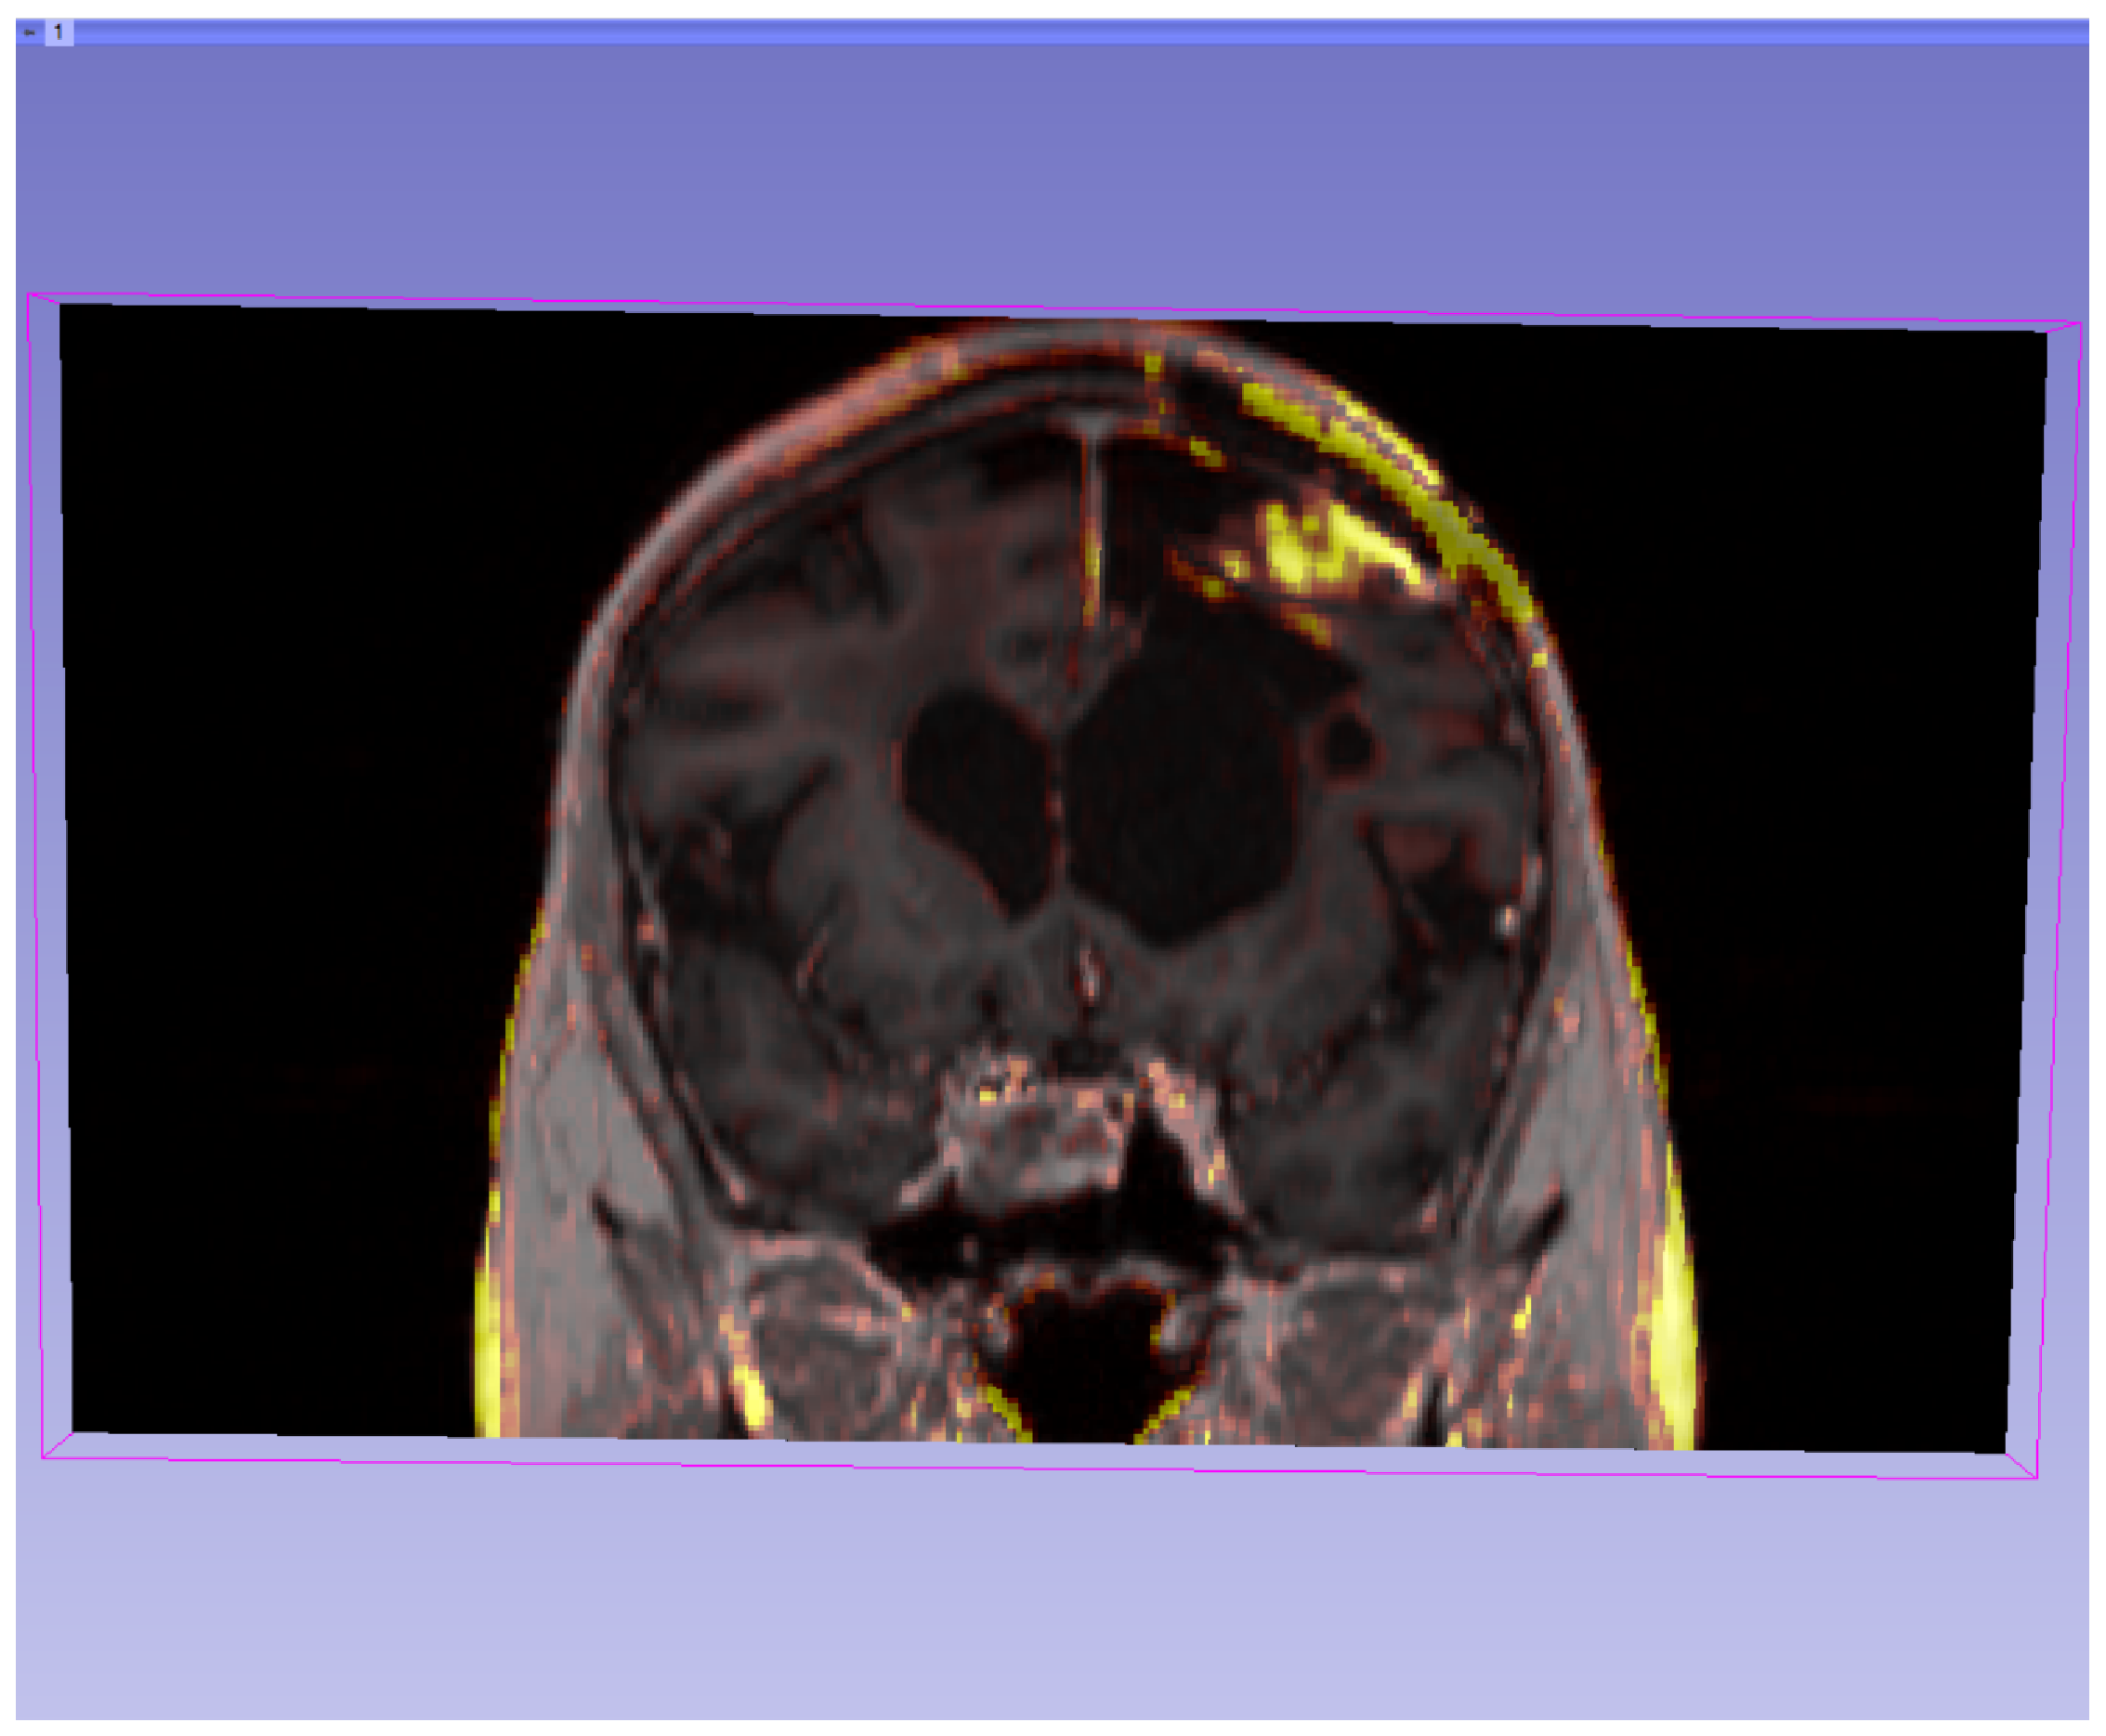
\includegraphics[scale=0.2]{/experiment_B2_P3/B2_Coronal.eps}
  \caption{Voxel-based method. Patient 3: Coronal plane}
  \label{B2_Coronal}
\end{figure}

\begin{figure}[H]
  \centering
  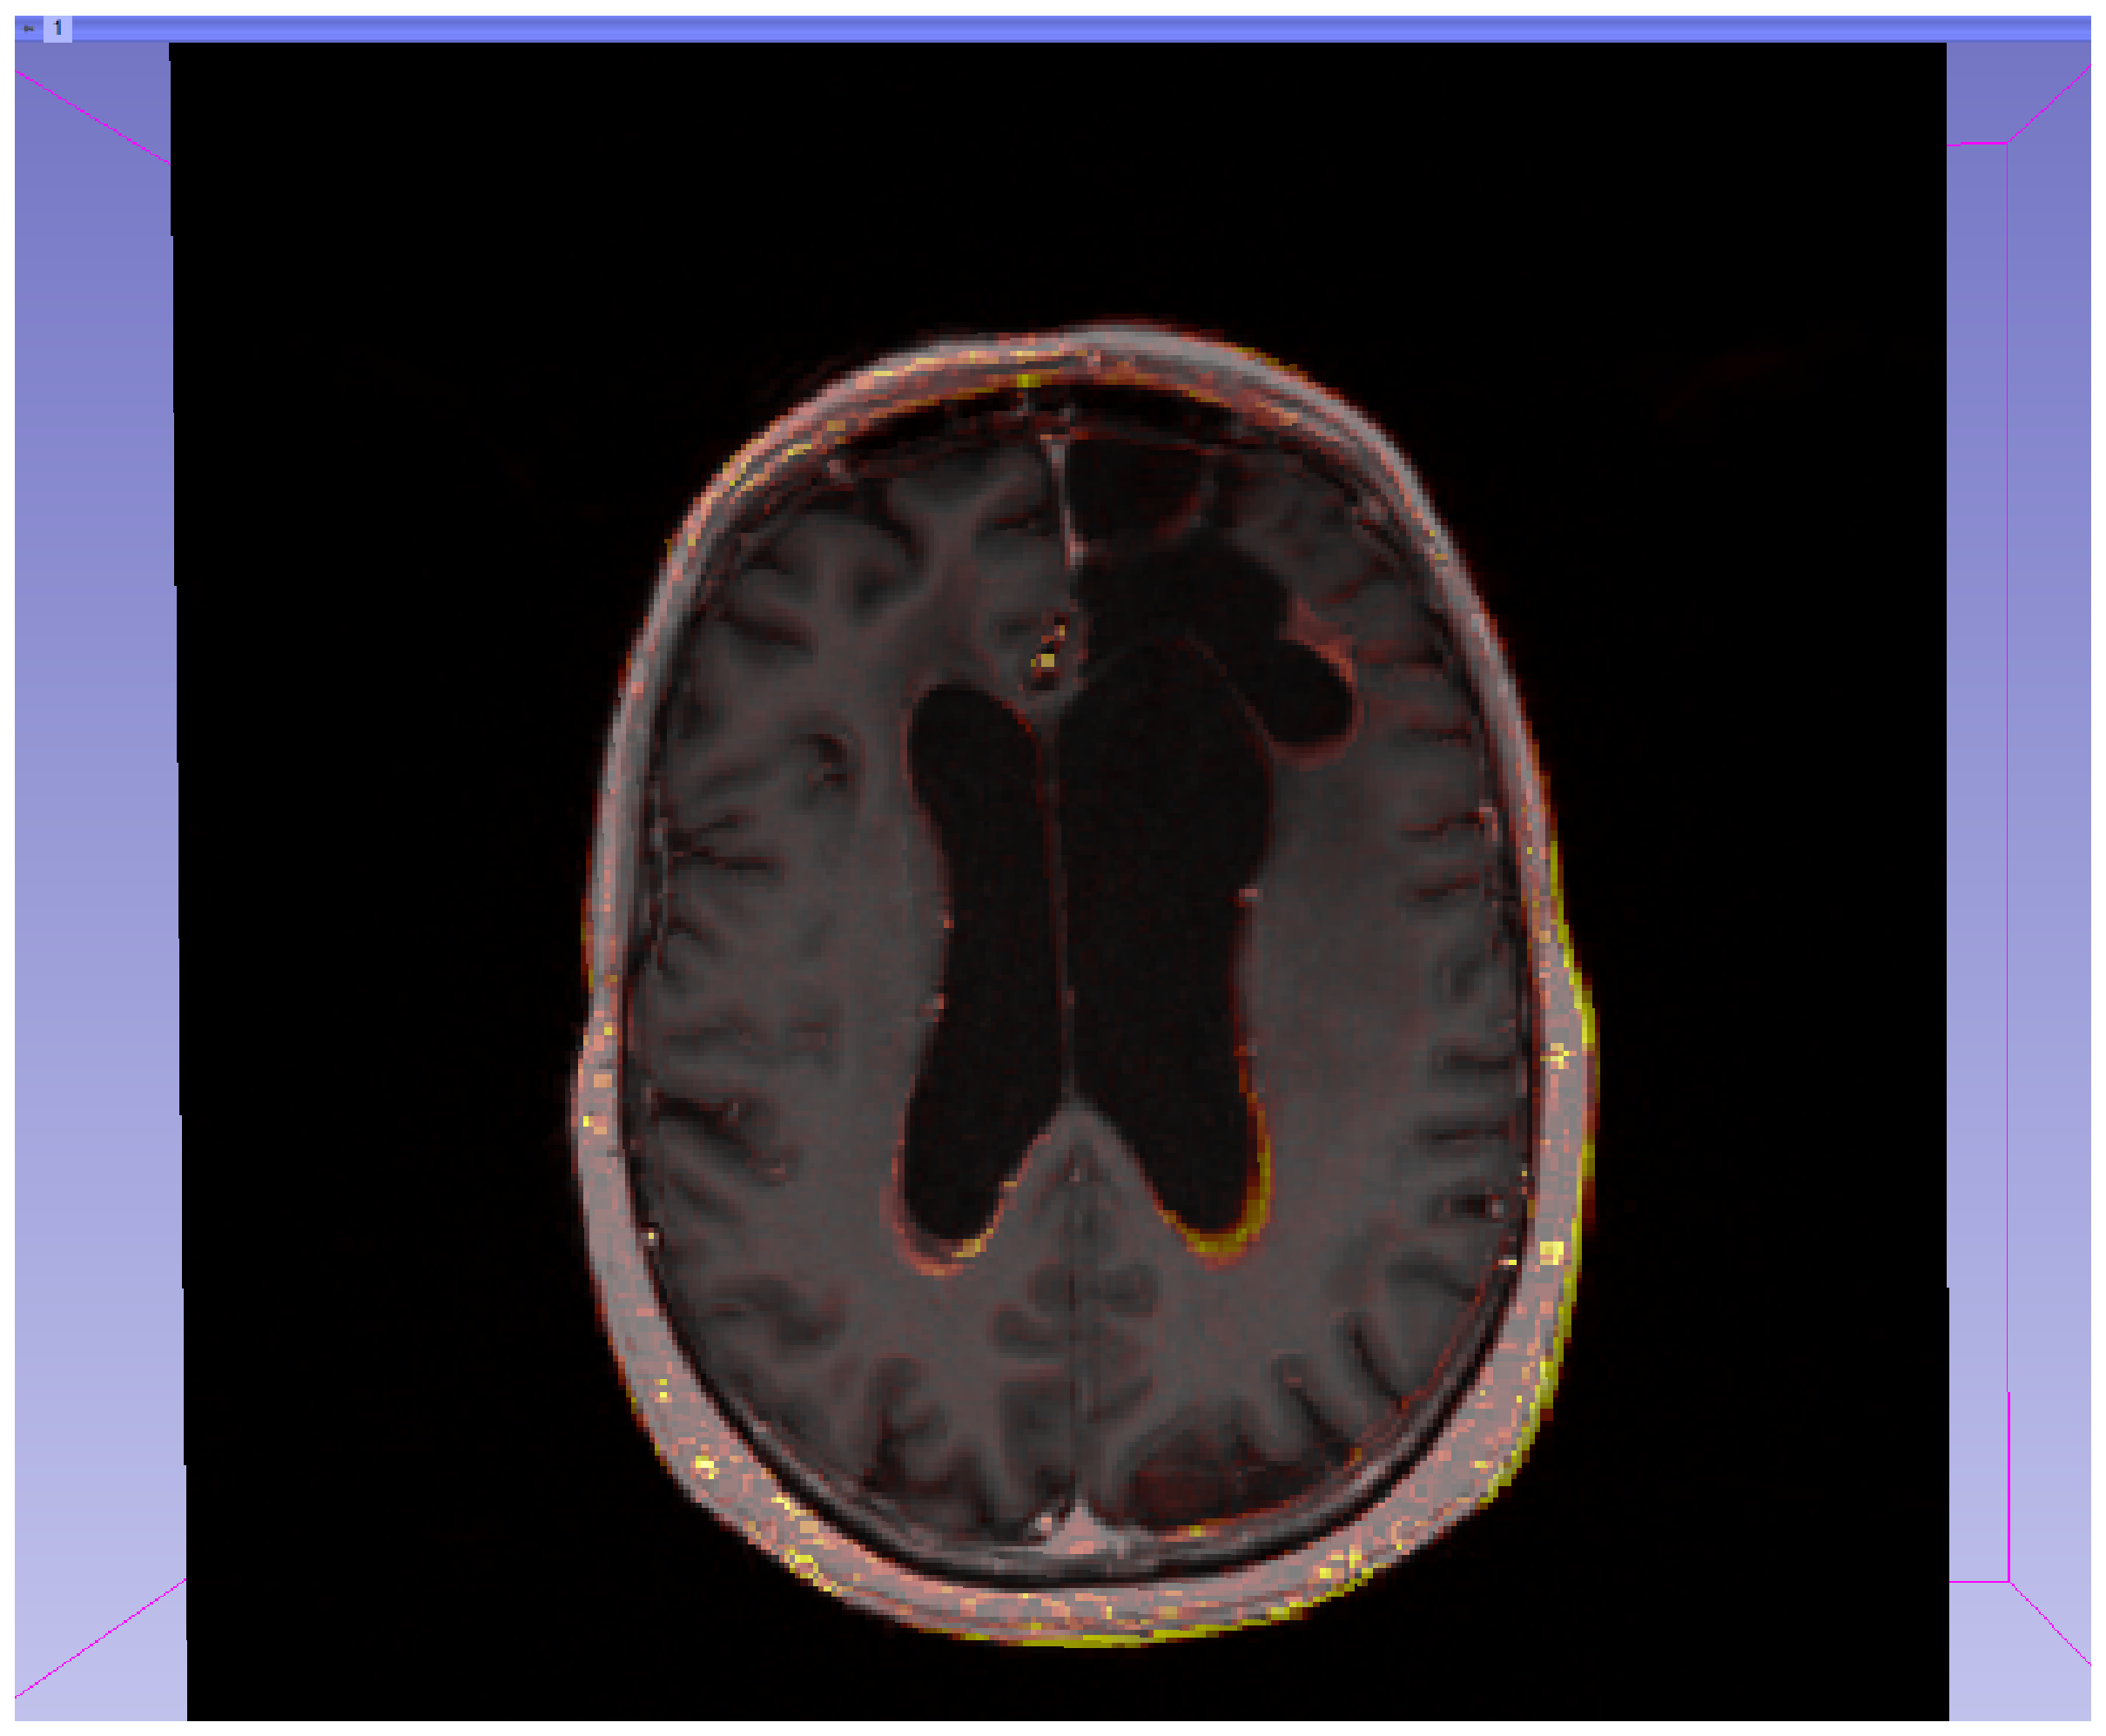
\includegraphics[scale=0.2]{/experiment_B2_P3/B2_Traversal1.eps}
  \caption{Voxel-based method. Patient 3: Traversal plane}
  \label{B2_Traversal1}
\end{figure}

\begin{figure}[H]
  \centering
  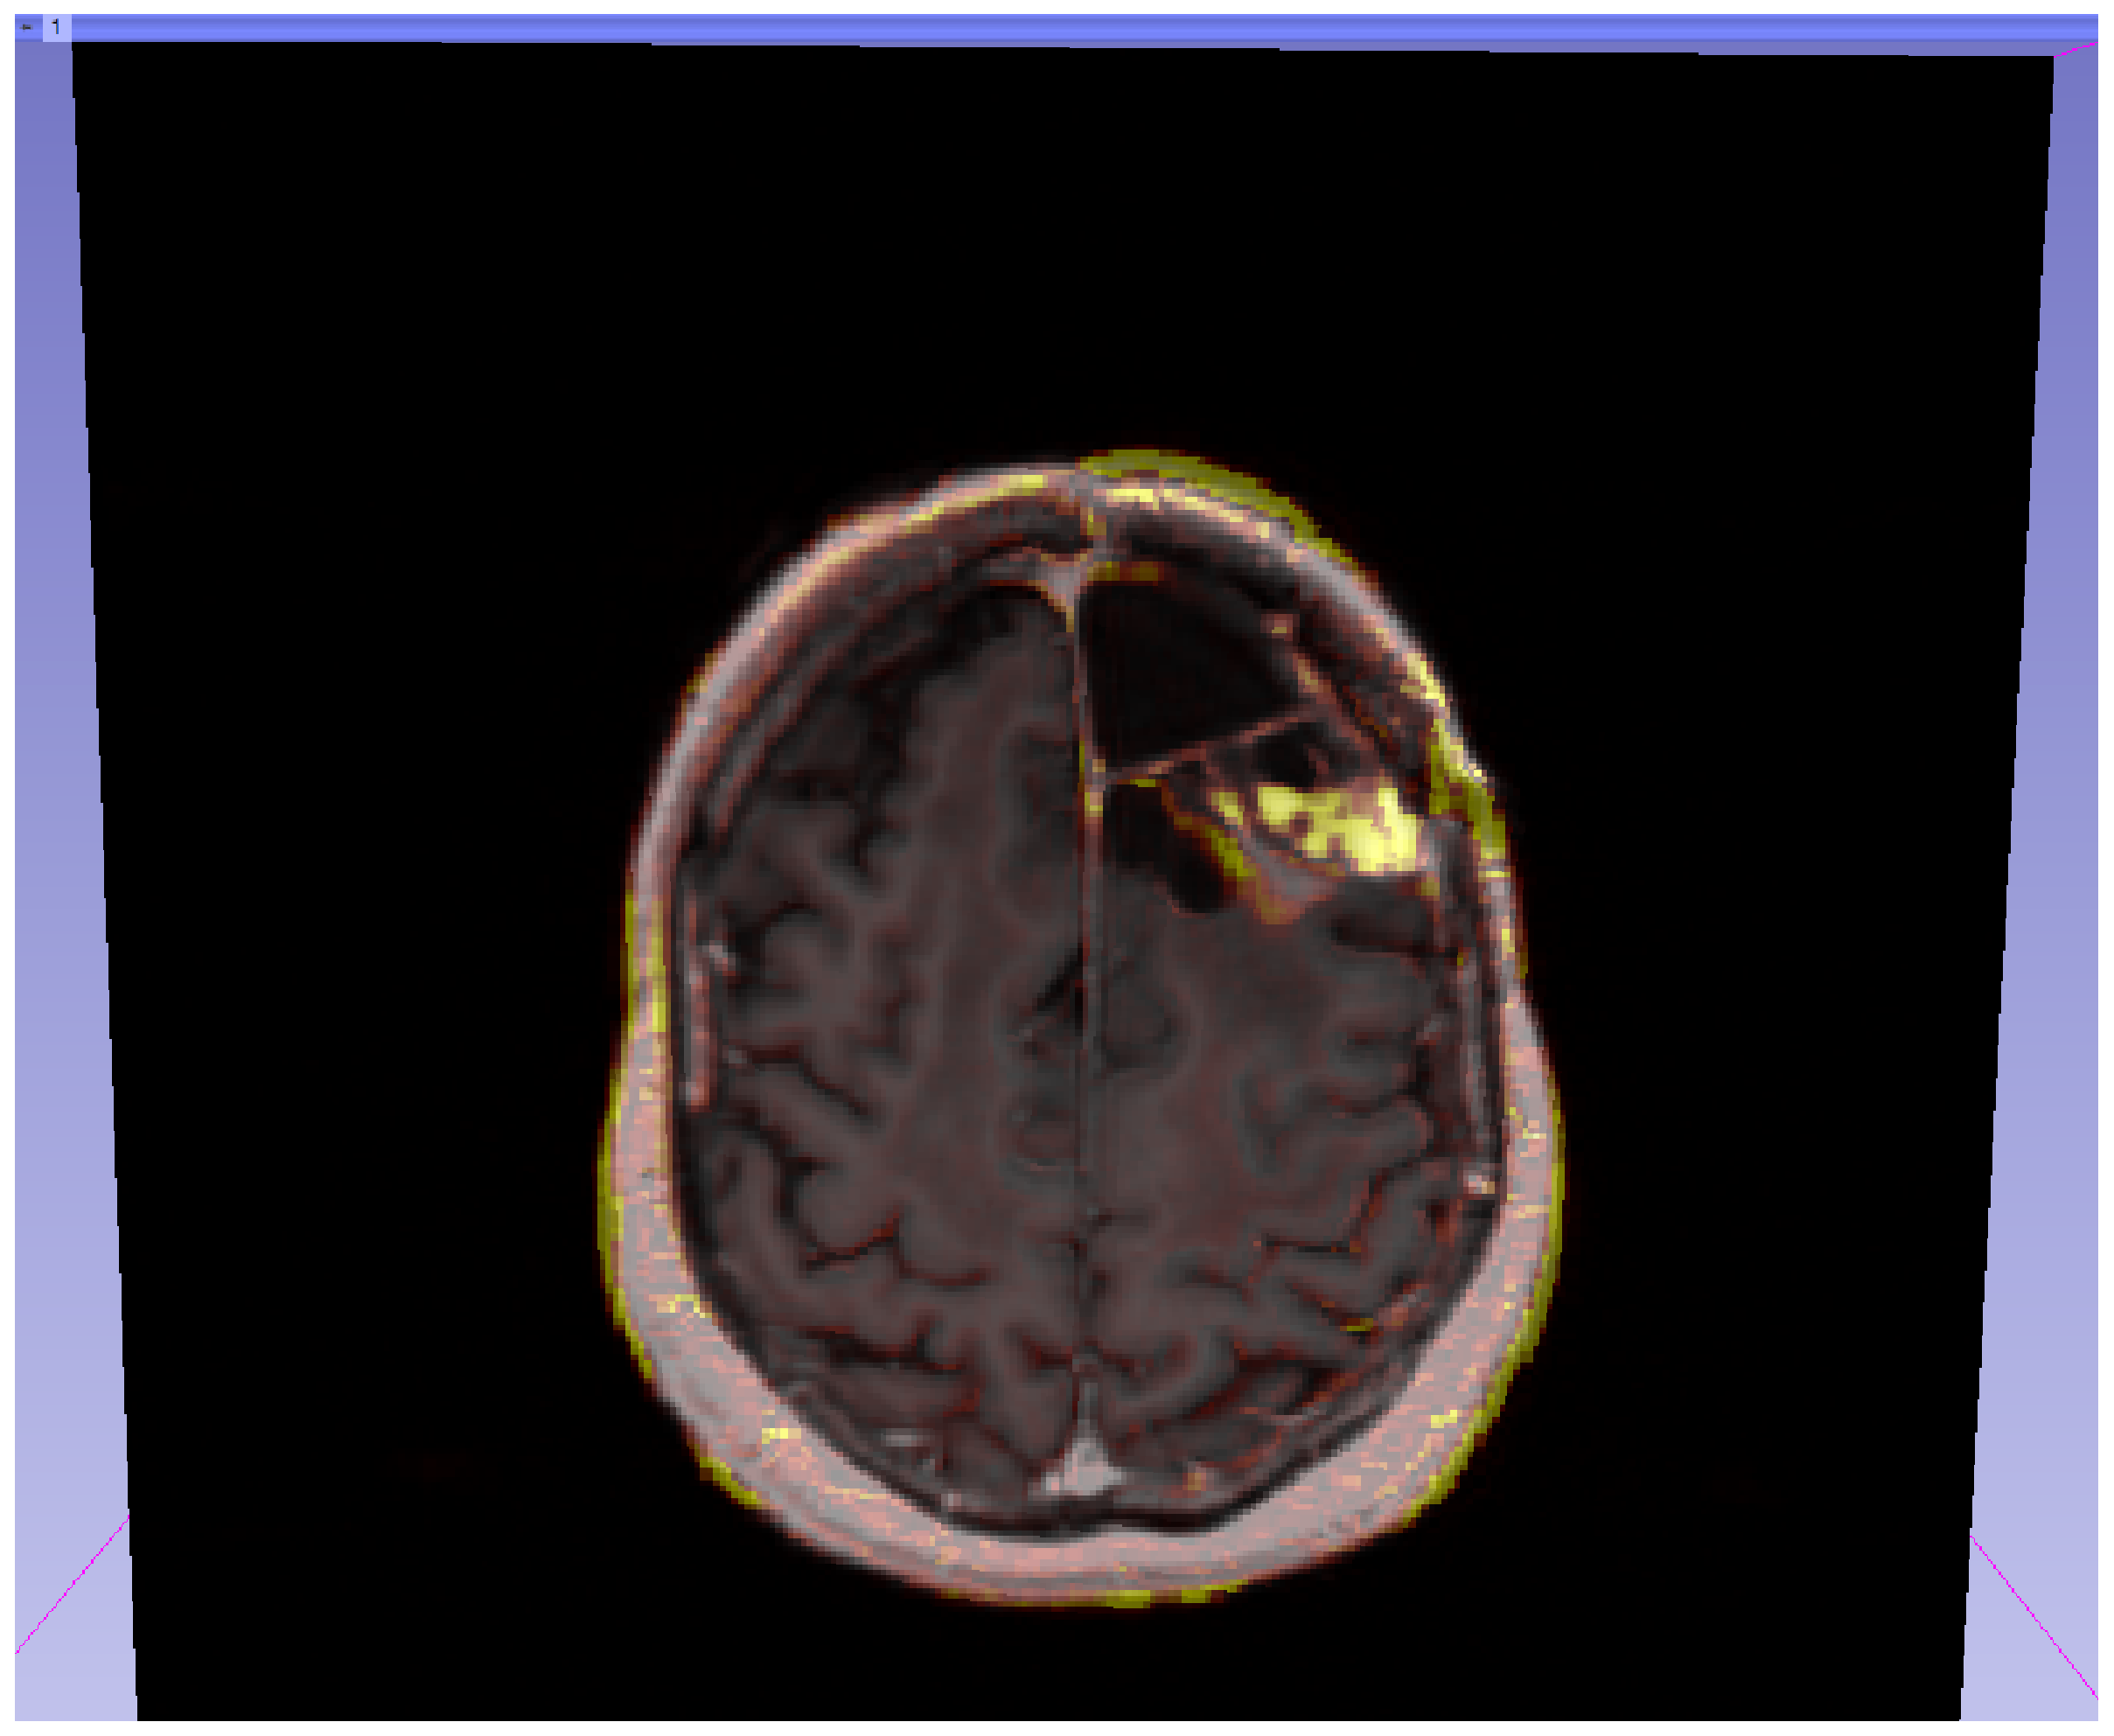
\includegraphics[scale=0.2]{/experiment_B2_P3/B2_Traversal2.eps}
  \caption{Voxel-based method. Patient 3: Upper traversal plane}
  \label{B2_Traversal2}
\end{figure}

\begin{figure}[H]
  \centering
  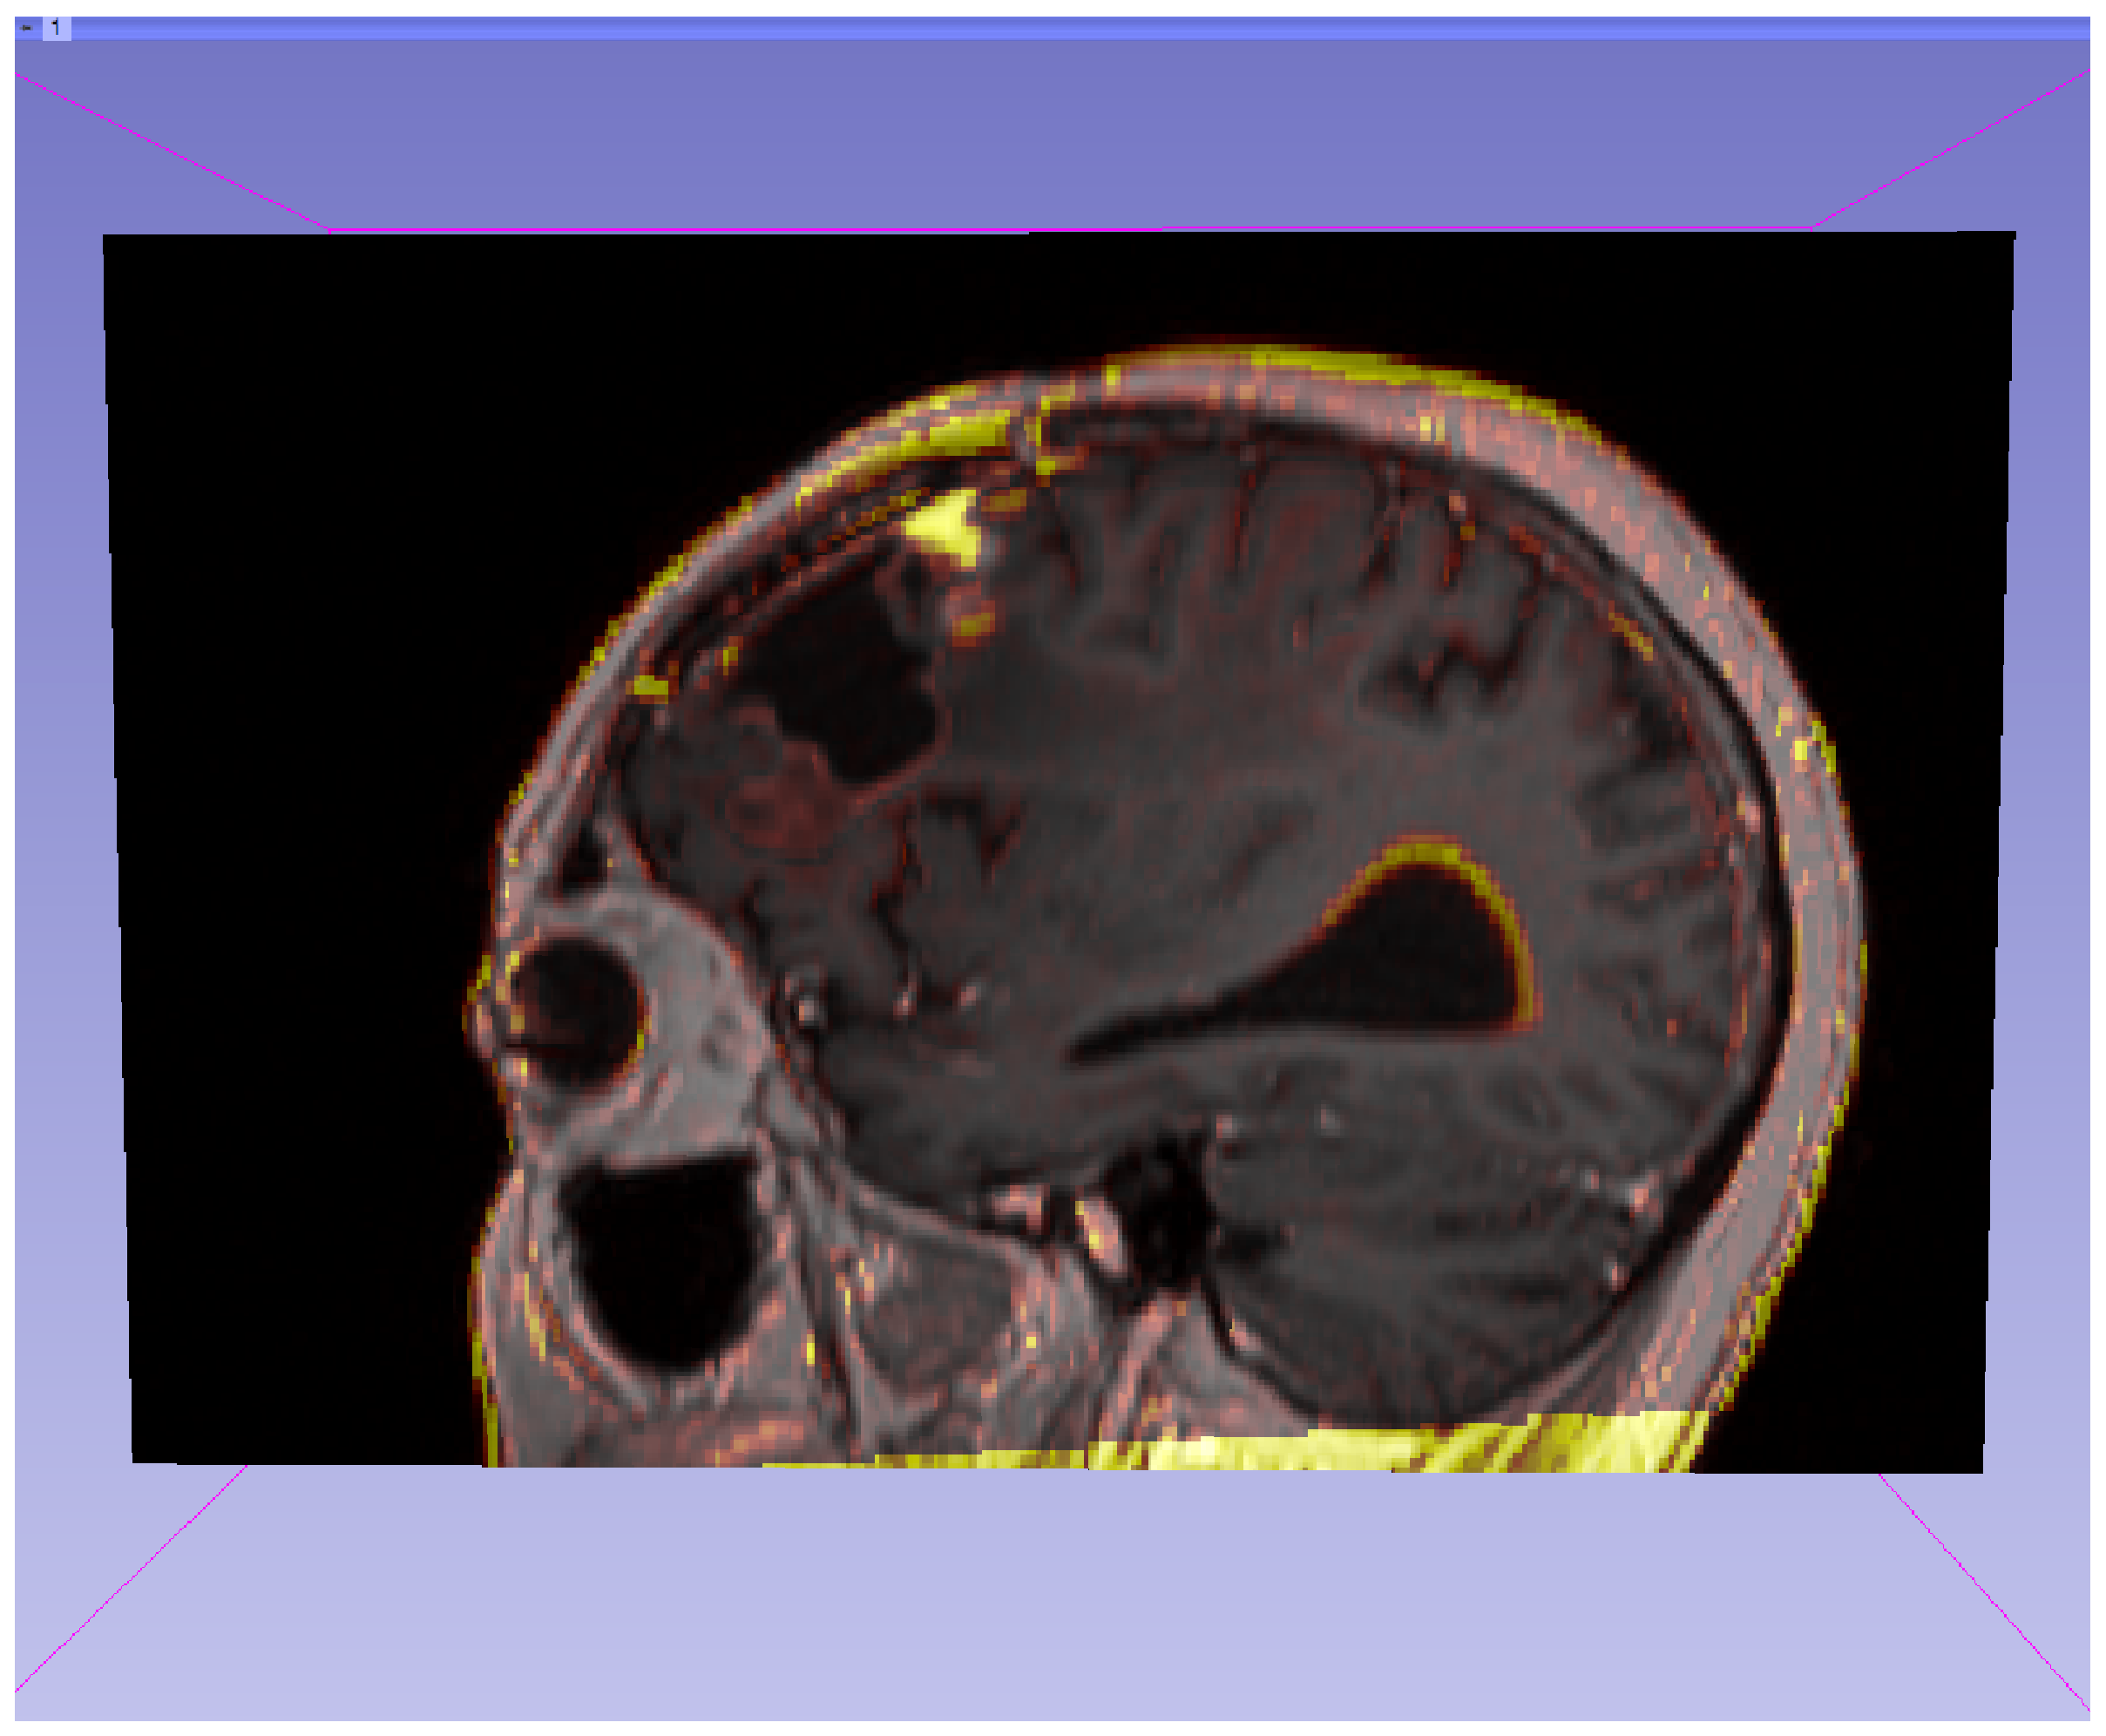
\includegraphics[scale=0.2]{/experiment_B2_P3/B2_Sagittal.eps}
  \caption{Voxel-based method. Patient 3: Sagittal plane}
  \label{B2_Sagittal}
\end{figure}


\subsubsection{Tensor-based Method}
This method also shows the expected difference due to the surgery
(correctly expressed as shrinkage, in green) which can be seen in the
images \ref{B2_TCoronal}, \ref{B2_TTraversal2} and \ref{B2_TSagittal}.

The image \ref{B2_TTraversal1} is showed for comparison with the
differences shown in image \ref{B2_Traversal1} in the previous
method. The tensor-based result doesn't show the exact same result;
however, some growth (in pink) can be seen. This could be attributed
to either inaccuracy of the method or to movement in the brain
consistent with the surgery.\\

Parameters used:
\begin{description}
\item \textit{Deformation field smoothing sigma:} 2.5
\item \textit{Shrinkage percentage:} 60
\item \textit{Growth percentage:} 50
\end{description}

\begin{figure}[H]
  \centering
  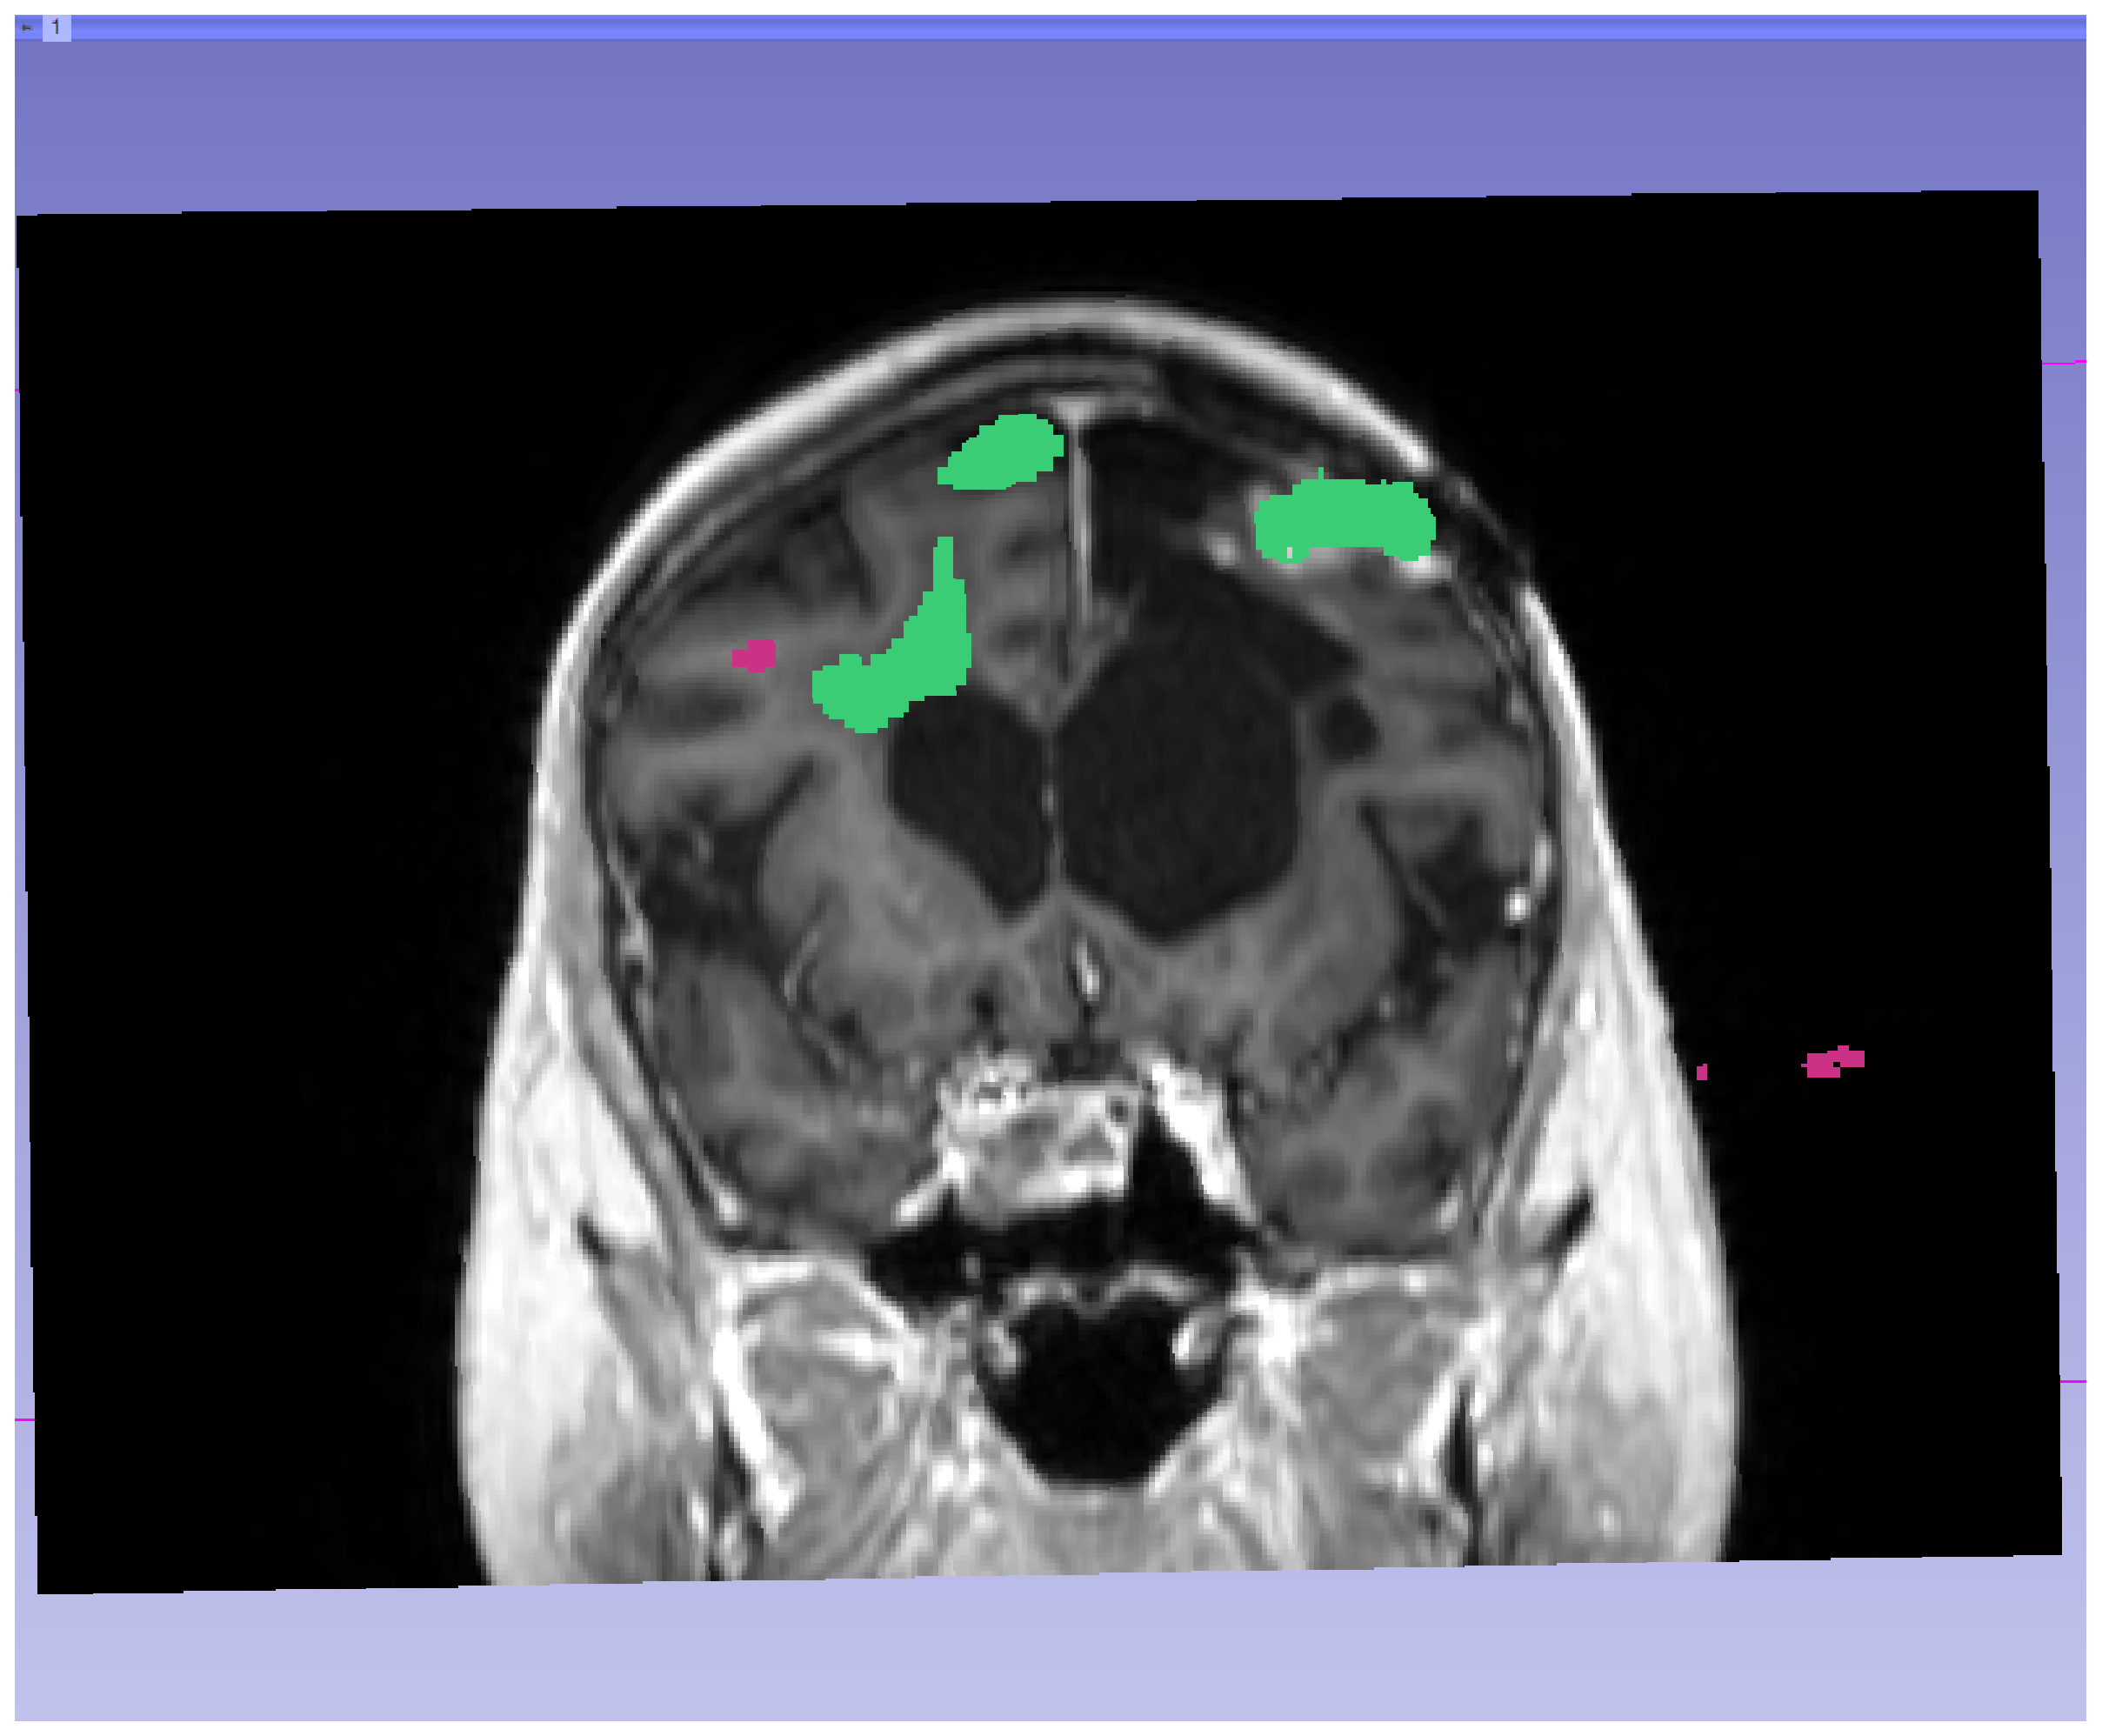
\includegraphics[scale=0.2]{/experiment_B2_P3/B2_Tensor_Coronal.eps}
  \caption{Tensor-based method. Patient 3: Coronal plane}
  \label{B2_TCoronal}
\end{figure}

\begin{figure}[H]
  \centering
  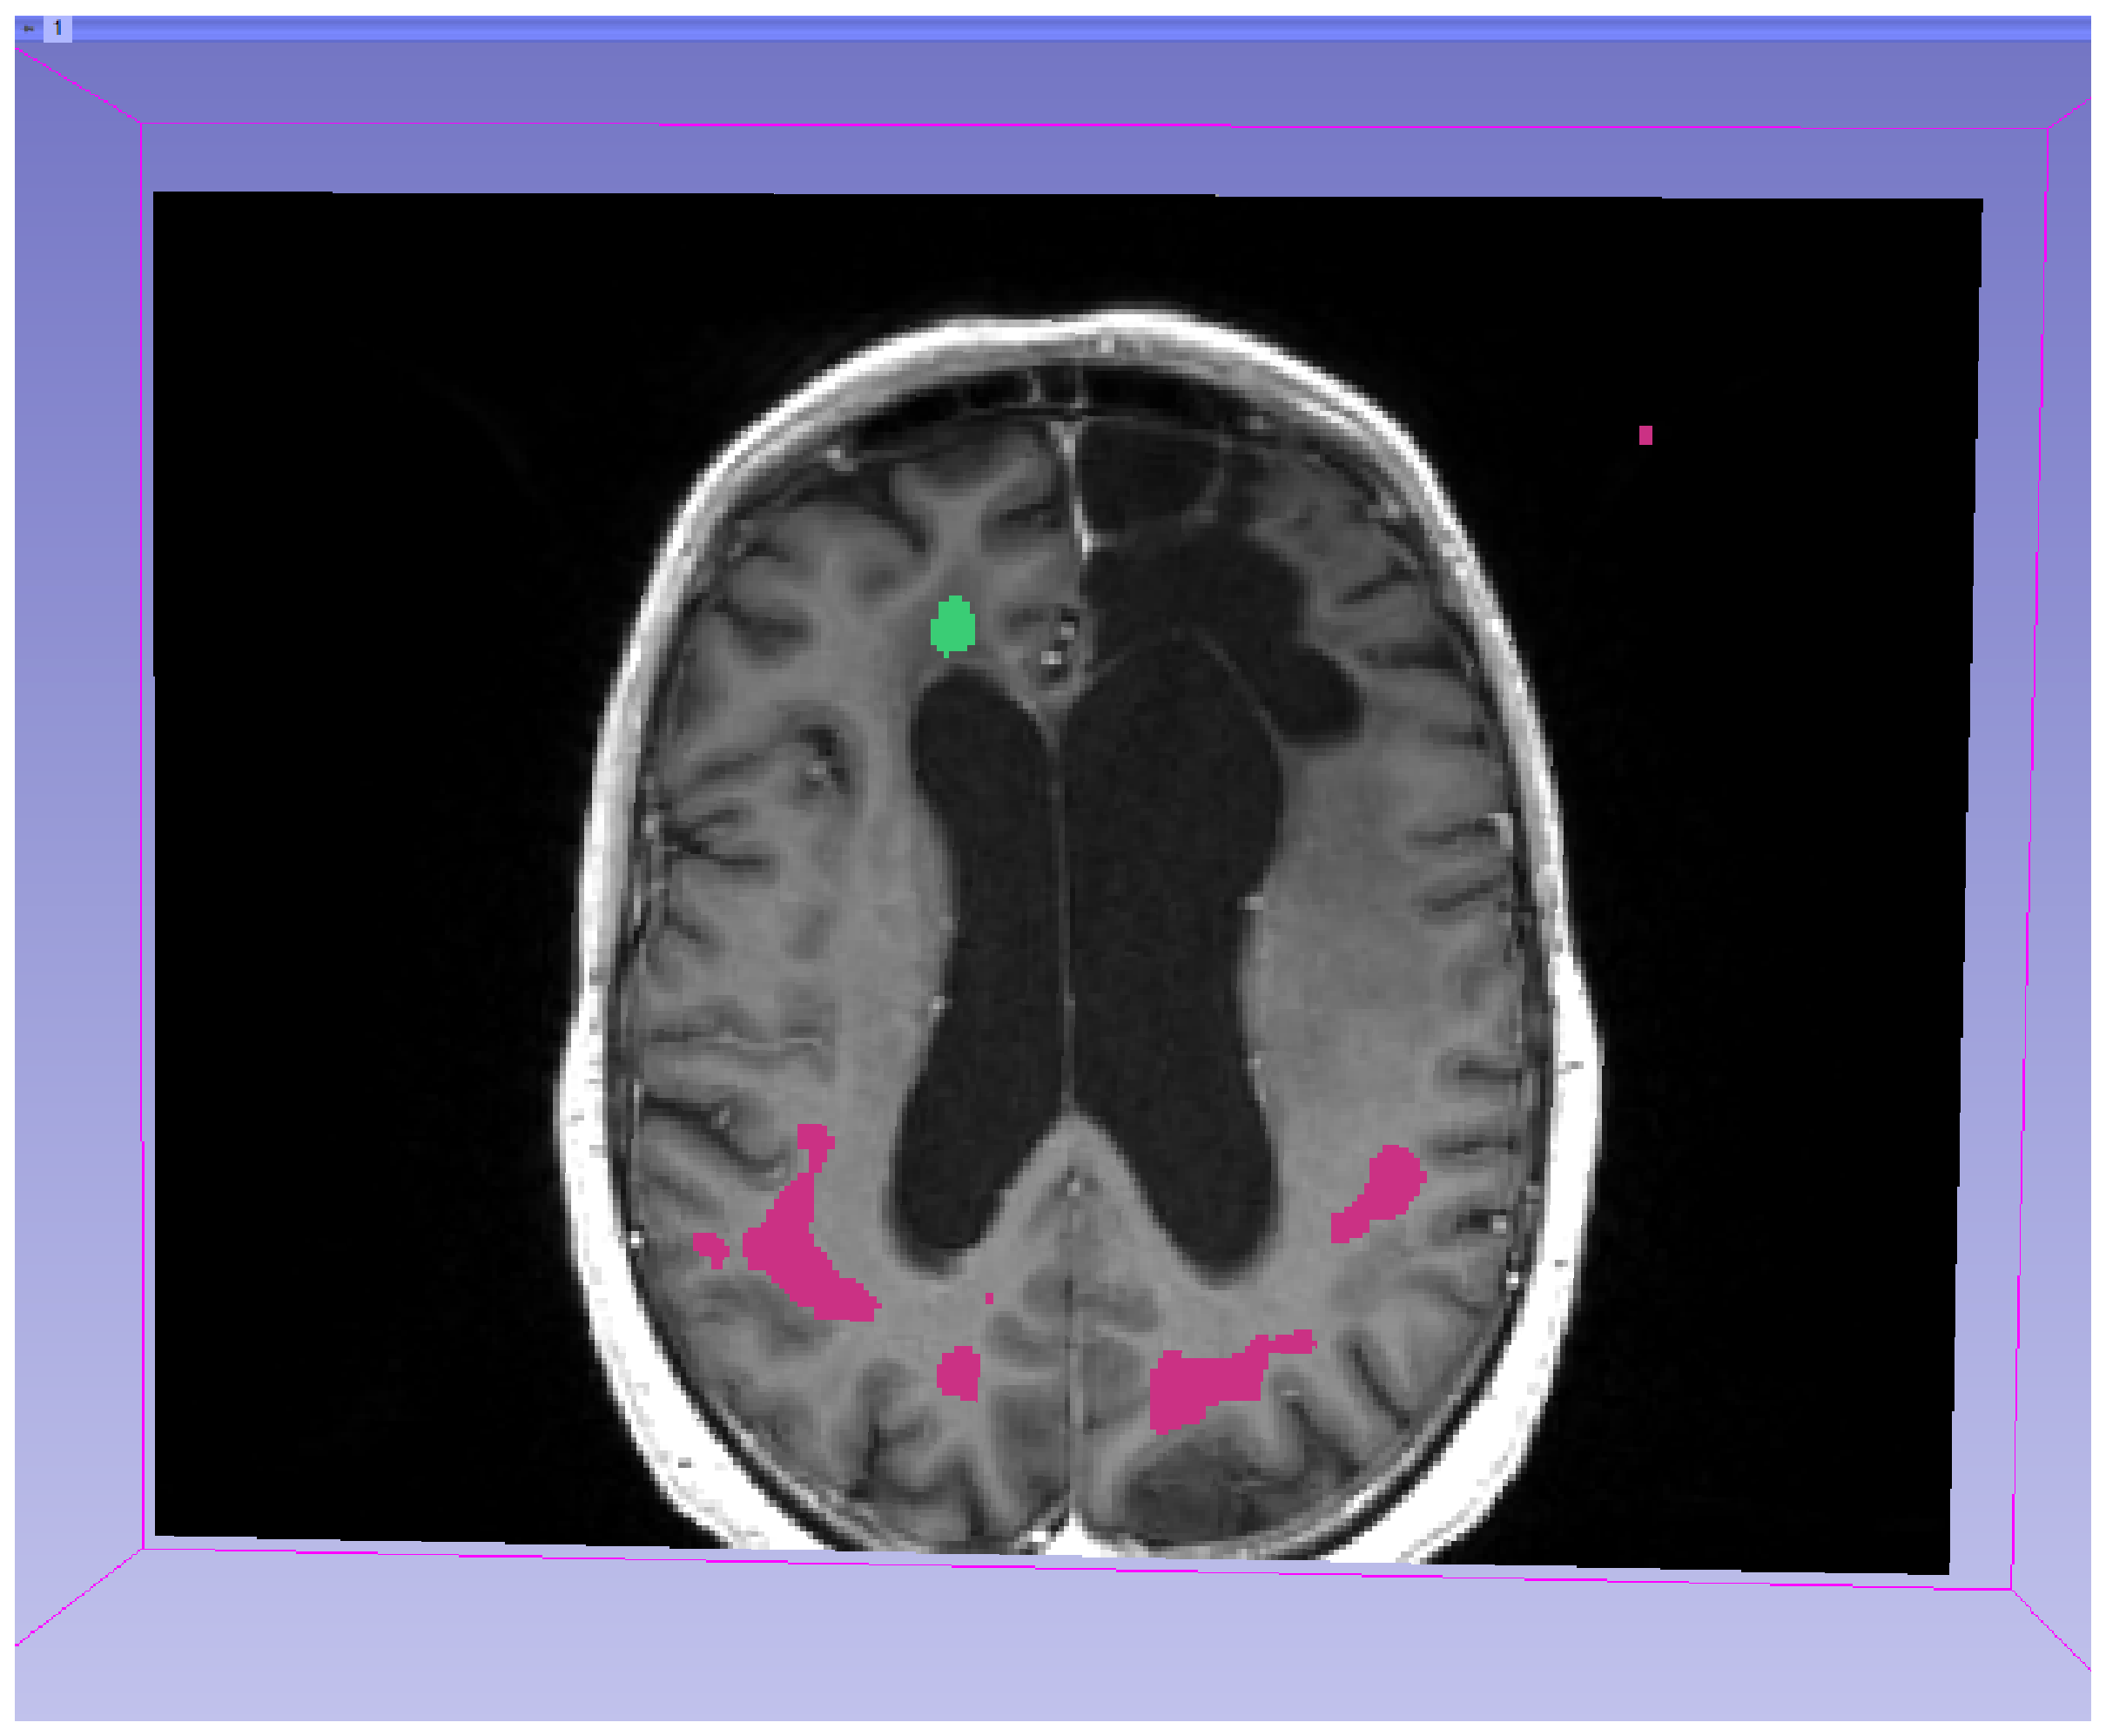
\includegraphics[scale=0.2]{/experiment_B2_P3/B2_Tensor_Traversal1.eps}
  \caption{Tensor-based method. Patient 3: Traversal plane}
  \label{B2_TTraversal1}
\end{figure}

\begin{figure}[H]
  \centering
  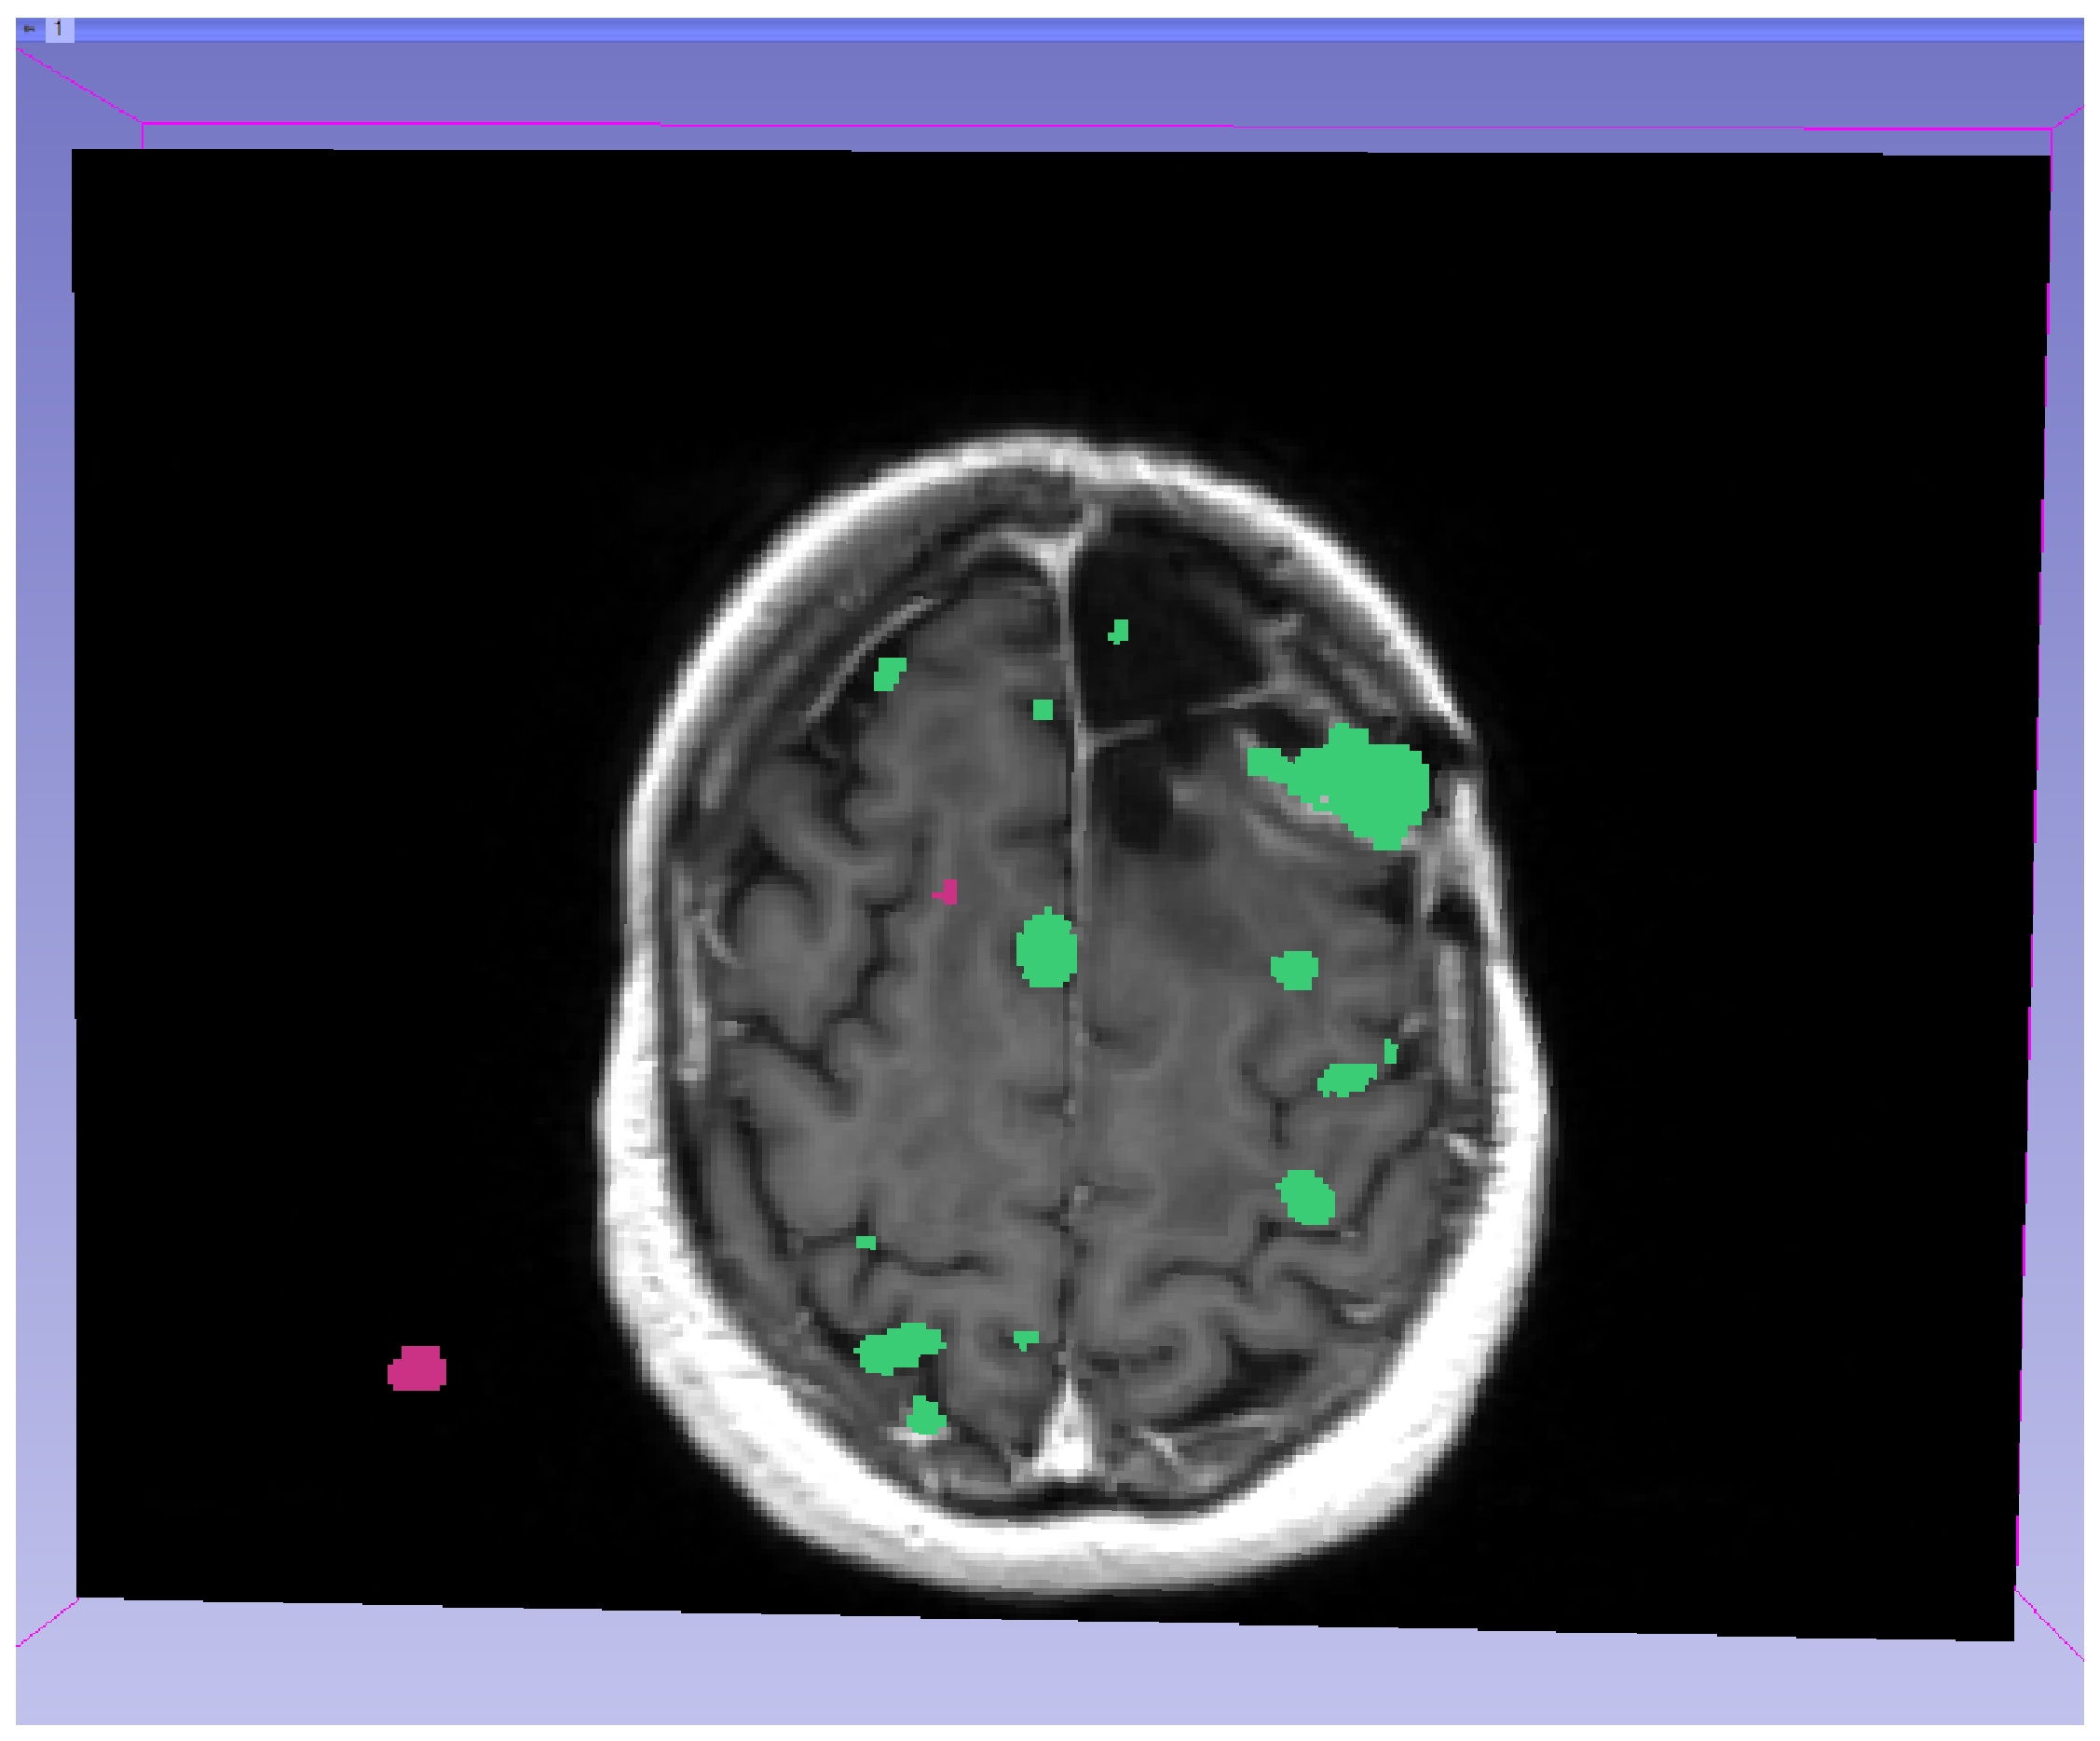
\includegraphics[scale=0.2]{/experiment_B2_P3/B2_Tensor_Traversal2.eps}
  \caption{Tensor-based method. Patient 3: Upper traversal plane}
  \label{B2_TTraversal2}
\end{figure}

\begin{figure}[H]
  \centering
  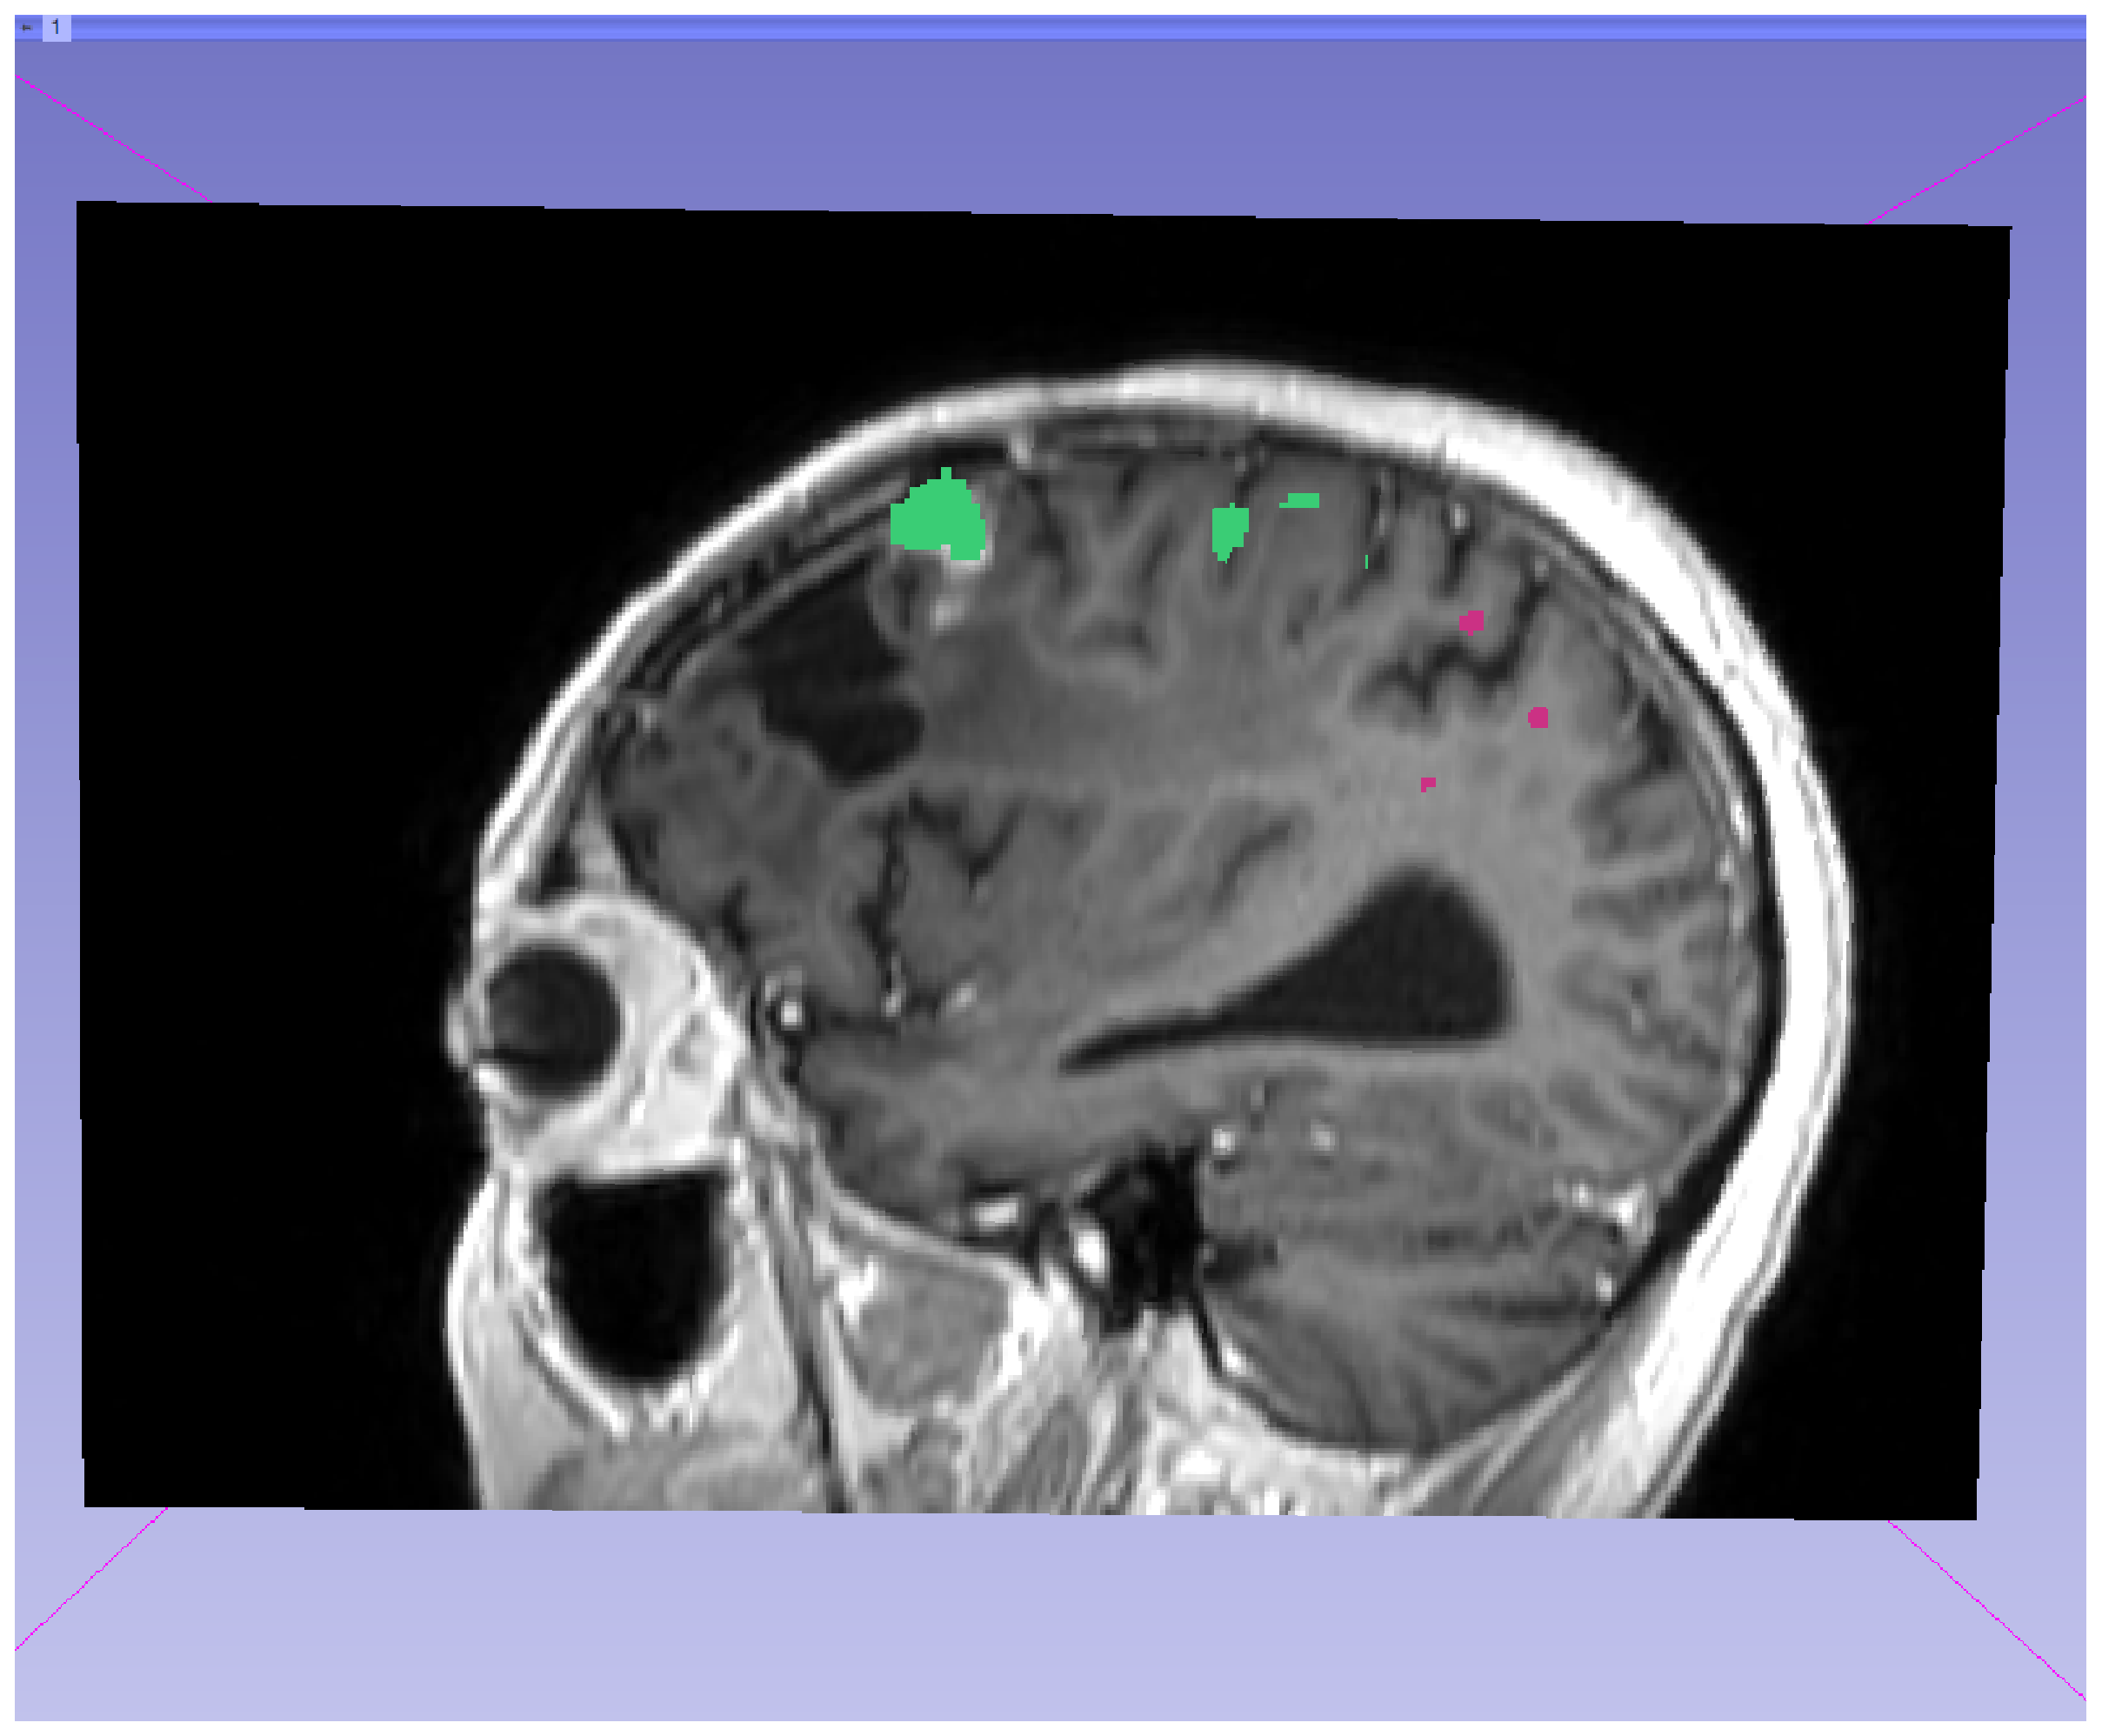
\includegraphics[scale=0.2]{/experiment_B2_P3/B2_Tensor_Sagittal.eps}
  \caption{Tensor-based method. Patient 3: Sagittal plane}
  \label{B2_TSagittal}
\end{figure}